%%%%% DOCUMENT CLASS
\documentclass[11pt]{article}

%%%%% IMPORTING PACKAGES
\usepackage{geometry} % page format
\usepackage{setspace} % page format
\usepackage{amsmath, amsthm, amssymb} % math stuff
\usepackage{mathtools} % math stuff
\usepackage{mathrsfs} % math stuff
\usepackage{empheq} % math stuff
\usepackage{cancel} % math stuff
\usepackage{tikz} % for making figures
\usepackage{graphicx} % for figures
\usepackage{placeins} % for figure placement
\usepackage{caption, subcaption} % for figures
\usepackage{enumitem} % for lists
\usepackage{verbatim} % for pasting .txt files
\usepackage{array} % table stuff
\usepackage{threeparttable} % table stuff
\usepackage{tabularx} % table stuff
\usepackage{multirow} % table stuff
\usepackage{colortbl} % table stuff
\usepackage{booktabs} % table stuff
\usepackage{pdfpages} % for importing pdfs
\usepackage{hyperref} % for hyperlinks
\usepackage{titletoc} % for TOC
\usepackage[table,dvipsnames]{xcolor} % for text coloring
\usepackage[backend=biber,sorting=none,style=numeric-comp]{biblatex} % for references
\usepackage{lipsum} % for filler
\usepackage{comment} % for comments
\usepackage{minted} % for code listings
% \usepackage{listings} % for code listings (alternative option)

%%%%% CONFIGURING PACKAGE SETTINGS
% paper size
\geometry{letterpaper,left=1in,top=1in,right=1in,bottom=1in}

% line spacing
% \singlespacing
\onehalfspacing
% \doublespacing
% \setstretch{1.25}

% graphics stuff
\graphicspath{ {./Figures/} }
\allowdisplaybreaks[1]

% links
\hypersetup{colorlinks=true, linkcolor=red, filecolor=magenta, urlcolor=black, citecolor=blue}

% adding bib
\addbibresource{bib.bib}

% list customization
\setlist[enumerate]{itemsep=1pt}

%%%%% CREATING CUSTOM COMMANDS
% custom page numbering
\newcommand{\mainmatter}{\clearpage\setcounter{page}{1}\pagenumbering{arabic}}
\newcommand{\appendixpagenumbering}{\clearpage\pagenumbering{arabic}\renewcommand{\thepage}{A-\arabic{page}}}

% TOC customization
\newcommand\innercontentsname[1]{%
Contents for section~\ref{#1}}

% custom table columns
\newcolumntype{P}[1]{>{\centering\arraybackslash}p{#1}}
\newcolumntype{M}[1]{>{\centering\arraybackslash}m{#1}}
\newcolumntype{R}[1]{>{\raggedleft\arraybackslash}m{#1}}
\renewcommand\tabularxcolumn[1]{m{#1}}

% whatever math operators we need
\DeclareMathOperator{\sgn}{sgn}
\DeclareMathOperator{\acos}{acos}
\DeclareMathOperator{\atantwo}{atan2}
\DeclareMathOperator{\spec}{Spec}
\DeclareMathOperator{\rank}{Rank}

%%%%% DOCUMENT
\begin{document}

%%%%% TITLE PAGE
\begin{titlepage}
\begin{center}
    \vspace*{\fill}
    {\Huge Engineering Collective Intelligence}\\
    {\large MAE 6870 Homework 3}

    \vspace{4\baselineskip}
    Daniel Whitman\\
    % Engineering Collective Intelligence (MAE 6870)\\
    11/24/2026
\end{center}

% \vspace{4\baselineskip}
% \noindent \textbf{ABSTRACT:}
% \noindent 

\vspace*{\fill}
\end{titlepage}

%%%%% ABSTRACT PAGE
% \clearpage
% \pagenumbering{gobble}
% \section*{ABSTRACT}
% \noindent Words

%%%%% ACTUAL REPORT
\mainmatter
\section*{AI STATEMENT}
I did not use AI for this assignment outside of the AI summary that Google provides when searching something up, which was all related to how to implement something in Python (e.g., how to plot a rectangle on a plot Python, etc.).

\section*{TEAM WORKLOAD}
For this homework, I (Daniel Whitman) completed \textbf{Part 1. Formation control}, while my partner (Julian McCafferty) completed \textbf{Part 2. Flocking with Robo-Boids}. We had no collaboration across the parts, and provided each other with our completed graphs and parameters from our own designed initial conditions, experiment conditions, etc. once we were completed with our part.

\section*{PROBLEM SOLUTIONS (Part 1: Formation control)}
\subsection*{A. Design and assemble a static formation}
\subsubsection*{1.}
Choose $N$ between 5 and 16 and design a planar formation shape; you are encouraged to be creative. \textbf{You may \underline{not} use a hexagon/circular formation that is already implemented in the provided example.} For your desired formation, design a (static, undirected, unweighted) communication graph $\mathcal G=(\mathcal V,\mathcal E)$ and show that under this choice, the formation is rigid. Plot your desired formation shape, write down the $(x,y)$ coordinate pair description, the associated pairwise distance constraint description, and the graph adjacency and Laplacian matrices corresponding to your communication graph.

\subsubsection*{ANSWER:}
For the static-formation control experiments, the formation that was design uses $N=8$ robots in a ``triangular'' shape, as seen in Figure \ref{fig:formation}. The $(x,y)$ coordinate description $p$ for each robot $i$ for this formation is, in meters $(m)$,
\begin{align}
    p_1&=(0,0) & p_2&=(0.4,0) & p_3&=(0.8,0) & p_4&=(0.4,0.4)\nonumber\\
    p_5&=(0,0.8) & p_6&=(-0.4,0.4) & p_7&=(-0.8,0) & p_8&=(-0.4,0)\label{eqn:p_ac}\,.
\end{align}

\begin{figure}[htb]
    \centering
    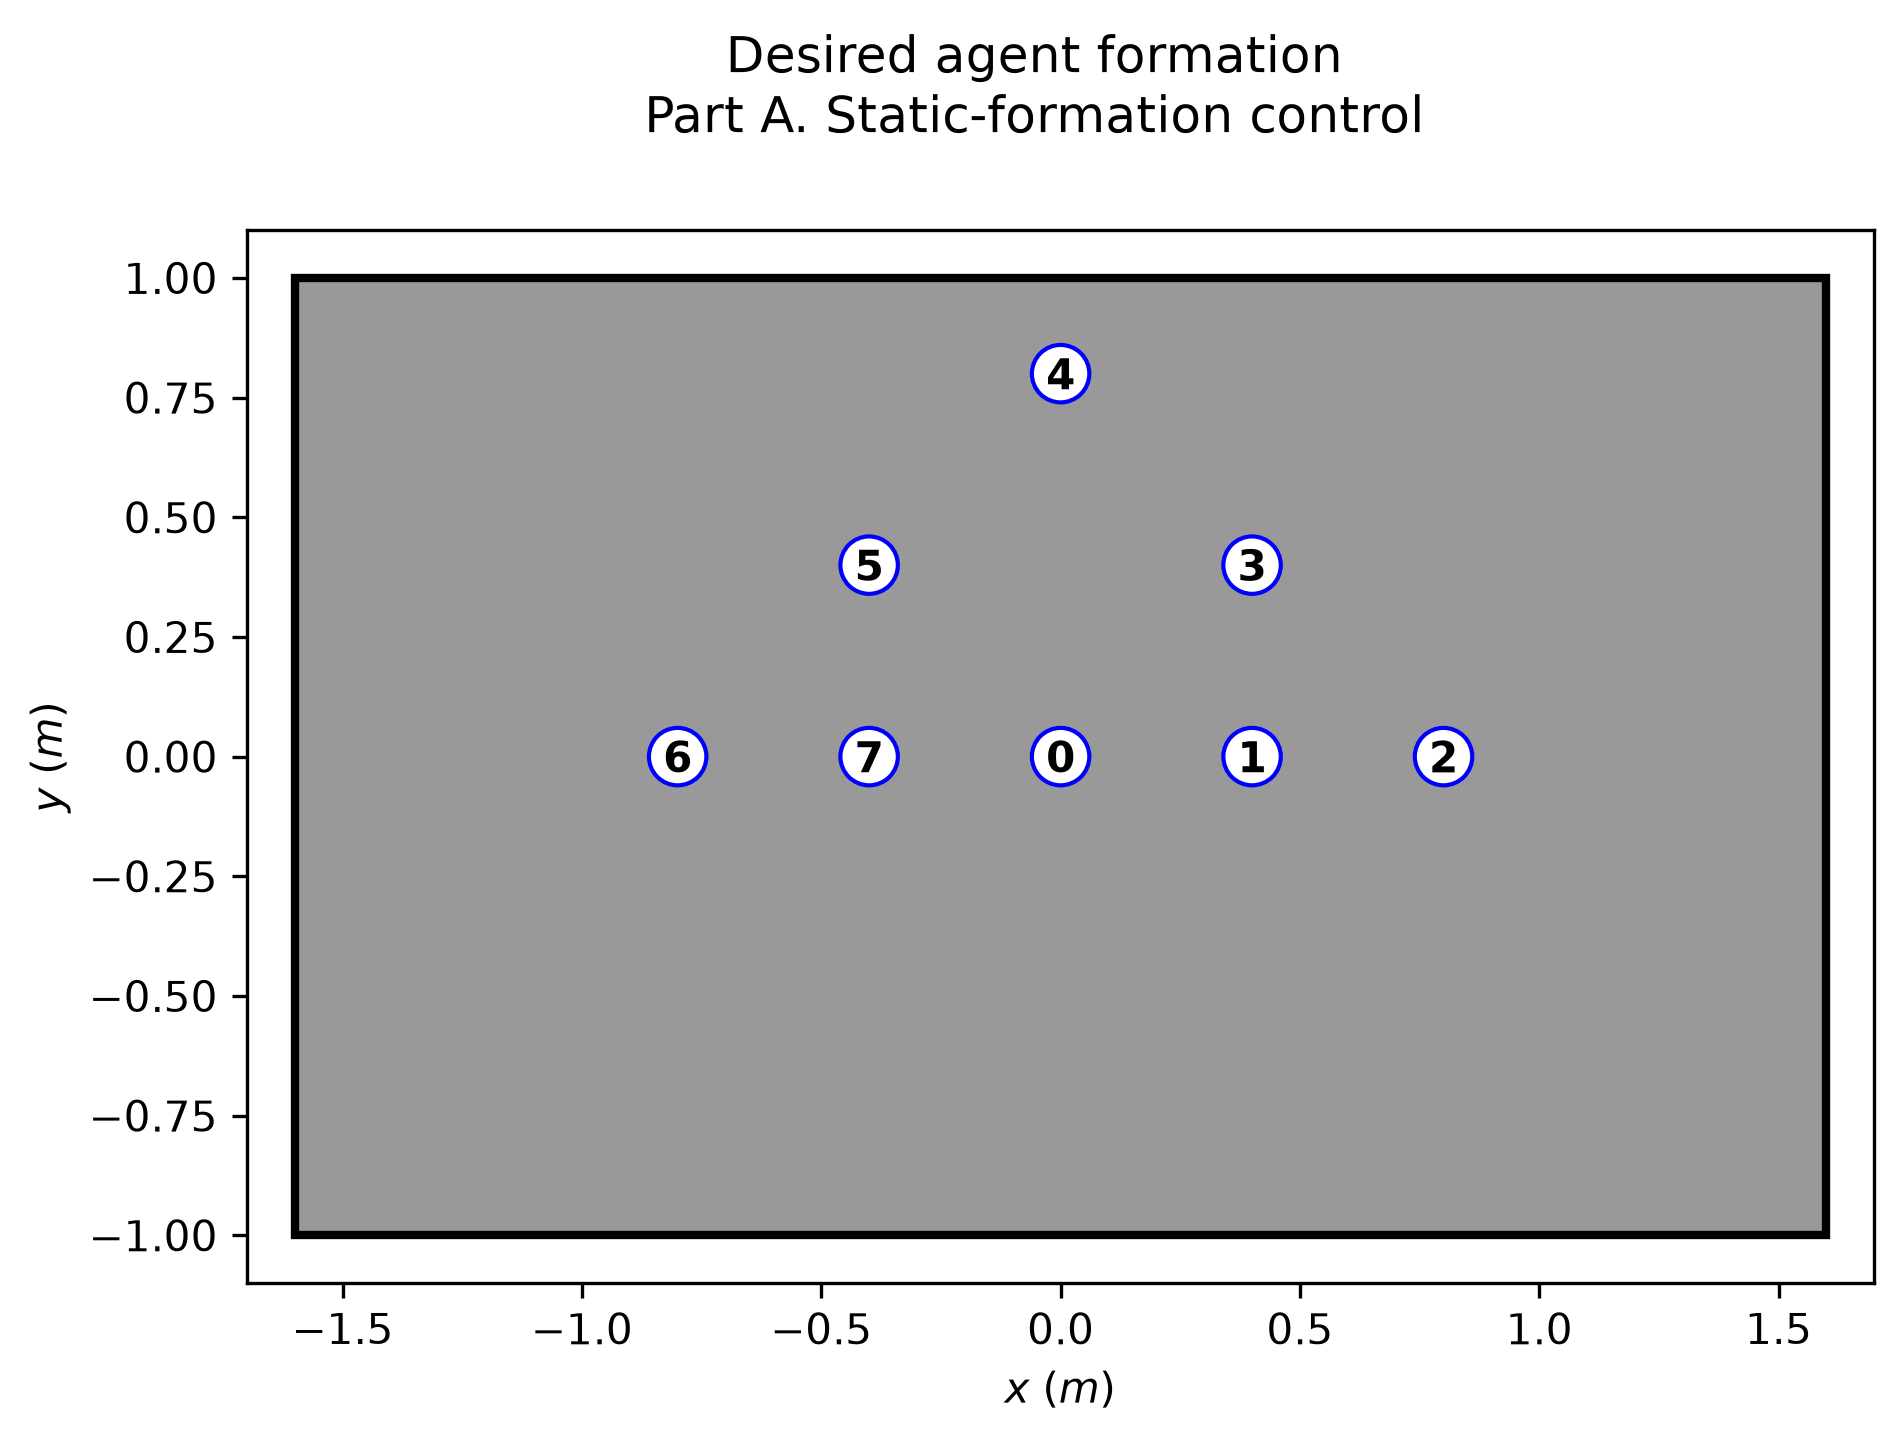
\includegraphics[width=0.5\textwidth]{Figures/formation.png}
    \captionsetup{justification=centering}
    \caption{Plot of desired formation in arena for distance-based and displacement-based formation control in static formation experiments.}
    \label{fig:formation}
\end{figure}

The communication graph $\mathcal G=(\mathcal V,\mathcal E)$ that was constructed can be shown with the pairwise distance constraint matrix,
\begin{align}\label{eqn:graph_ac}
    d_{ij}^{a,c}&=\begin{pmatrix}
        0 & 0.4 & 0 & 0.4\sqrt 2 & 0.8 & 0.4\sqrt 2 & 0 & 0.4\\
        0.4 & 0 & 0.4 & 0.4 & 0 & 0 & 0 & 0\\
        0 & 0.4 & 0 & 0.4\sqrt 2 & 0 & 0 & 1.6 & 0\\
        0.4\sqrt 2 & 0.4 & 0.4\sqrt 2 & 0 & 0.4\sqrt 2 & 0 & 0 & 0\\
        0.8 & 0 & 0 & 0.4\sqrt 2 & 0 & 0.4\sqrt 2 & 0 & 0\\
        0.4\sqrt 2 & 0 & 0 & 0 & 0.4\sqrt 2 & 0 & 0.4\sqrt 2 & 0.4\\
        0 & 0 & 1.6 & 0 & 0 & 0.4\sqrt 2 & 0 & 0.4\\
        0.4 & 0 & 0 & 0 & 0 & 0.4 & 0.4 & 0
    \end{pmatrix}\,,
\end{align}
where a value of 0 in row $i$ column $j$ shows that there is no communication $i\cancel{\iff}j$. With this matrix, the formation is \textit{rigid}, which can be seen by computing the rank of the rigidity matrix,
\begin{align*}
    R(p)&=\frac{\partial f}{\partial p}\in\mathbb R^{|\mathcal E|\times2N}\,, & \text{where }f(p)&=\left(\frac12\|p_i-p_j\|^2\right)_{i,j\in\mathcal E}\,,
\end{align*}
where $p=(p_1^T,\dots,p_N^T)^T$, with $p_i\in\mathbb R^2$ being the position of robot $i$ in the formation from (\ref{eqn:p_ac}). With this matrix, each row $R_{ij}$ corresponds to a communication edge with values
\begin{align*}
    R_{ij}(p)&=\begin{pmatrix}
        0 & \dots & (p_i-p_j)^T & \dots & (p_j-p_i)^T & \dots & 0
    \end{pmatrix}\,.
\end{align*}
The rigid condition is given by the rank of $R$, where the formation is \textit{rigid} if
\begin{align*}
    \rank(R(p))&=2N-3\,.
\end{align*}
For the described formation/graph, the formation rank was 13, so for $N=3$, this is sufficient. One thing to notice, however, is that there is actually a \textit{redundant} edge in the graph (14 edges instead of 13 edges), given between robot 2 and 6 with a constraint of $1.6\ m$. The addition of this edge was to help with experiment convergence, where, without it, depending on the initial conditions, robots 2 and 6 may end on the same ``side'' of the triangle and have no way to separate (identical to the triangle ``folding'' in half). We will explore this phenomenon in Part C.

Finally, for the graph (\ref{eqn:graph_ac}), the graph adjacency and Laplacian matrices are
\begin{align}\label{eqn:al_ac}
    A&=\begin{pmatrix}
        0 &  1 &  0 &  1 &  1 & 1 & 0 & 1\\
        1 &  0 &  1 &  1 &  0 & 0 & 0 & 0\\
        0 &  1 &  0 &  1 &  0 & 0 & 1 & 0\\
        1 &  1 &  1 &  0 &  1 & 0 & 0 & 0\\
        1 &  0 &  0 &  1 &  0 & 1 & 0 & 0\\
        1 &  0 &  0 &  0 &  1 & 0 & 1 & 1\\
        0 &  0 &  1 &  0 &  0 & 1 & 0 & 1\\
        1 &  0 &  0 &  0 &  0 & 1 & 1 & 0
    \end{pmatrix} & L&=\begin{pmatrix}
         5 & -1 &  0 & -1 & -1 & -1 &  0 & -1\\
        -1 &  3 & -1 & -1 &  0 &  0 &  0 &  0\\
         0 & -1 &  3 & -1 &  0 &  0 & -1 &  0\\
        -1 & -1 & -1 &  4 & -1 &  0 &  0 &  0\\
        -1 &  0 &  0 & -1 &  3 & -1 &  0 &  0\\
        -1 &  0 &  0 &  0 & -1 &  4 & -1 & -1\\
         0 &  0 & -1 &  0 &  0 & -1 &  3 & -1\\
        -1 &  0 &  0 &  0 &  0 & -1 & -1 &  3
    \end{pmatrix}\,.
\end{align}

\FloatBarrier
\subsubsection*{2.}
In code, implement a displacement-based and a distance-based formation control algorithm that enables the group of $N$ agents to reach the shape you designed. For the distance-based algorithm, you may build on the \texttt{formation\_control} example provided in the Robotarium Github repository. Run each algorithm in the provided simulator and in the Robotarium hardware, from a set of shared initial conditions. In your report, plot the trajectories for each of the runs (four total, two simulated and two hardware) as well as the distance constraint error over time, defined as
\begin{align*}
    E_d(t)&=\left[\frac{1}{|\mathcal E|}\sum_{(i,j)\in\mathcal E}(\|p_j(t)-p_i(t)\|-d_{ij})^2\right]^{1/2}\,,
\end{align*}
where $\mathcal E$ is the edge set in the communication graph, $p_i(t)\in\mathbb R^2$ is the position of robot $i$ at time $t$, and $d_{ij}$ is the desired distance between agents $i$ and $j$ in your formation. For both strategies also plot the square error between simulated and real robot positions, starting from shared initial conditions
\begin{align*}
    E_{sim}(t)&=\sum_{i\in\mathcal V}\|p_i^{real}(t)-p_i^{sim}(t)\|^2\,.
\end{align*}
How do the two formation strategies compare?

\subsubsection*{ANSWER:}
For the desired formation in (\ref{eqn:p_ac}) and the graph with pairwise distance constraints given in (\ref{eqn:graph_ac}), both the distance-based formation control and displacement-based formation control algorithms were tested in both simulation and hardware. The trajectories for the experiments are given in Figure \ref{fig:traj_a}. While it is not so obvious from directly observing the plots, both methods \textit{were} able to reach the desired formation! However, in the distance-based formation, as there is no notion of a ``global reference'', the orientation/position of the final state did not match the coordinates from (\ref{eqn:p_ac}), while in the displacement-based orientation, the orientation of the formation was correct (although it was shifted vertically ``down'' with respect to (\ref{eqn:p_ac})).

\begin{figure}[htb]
    \centering
    \begin{subfigure}[t]{0.45\textwidth}
        \centering
        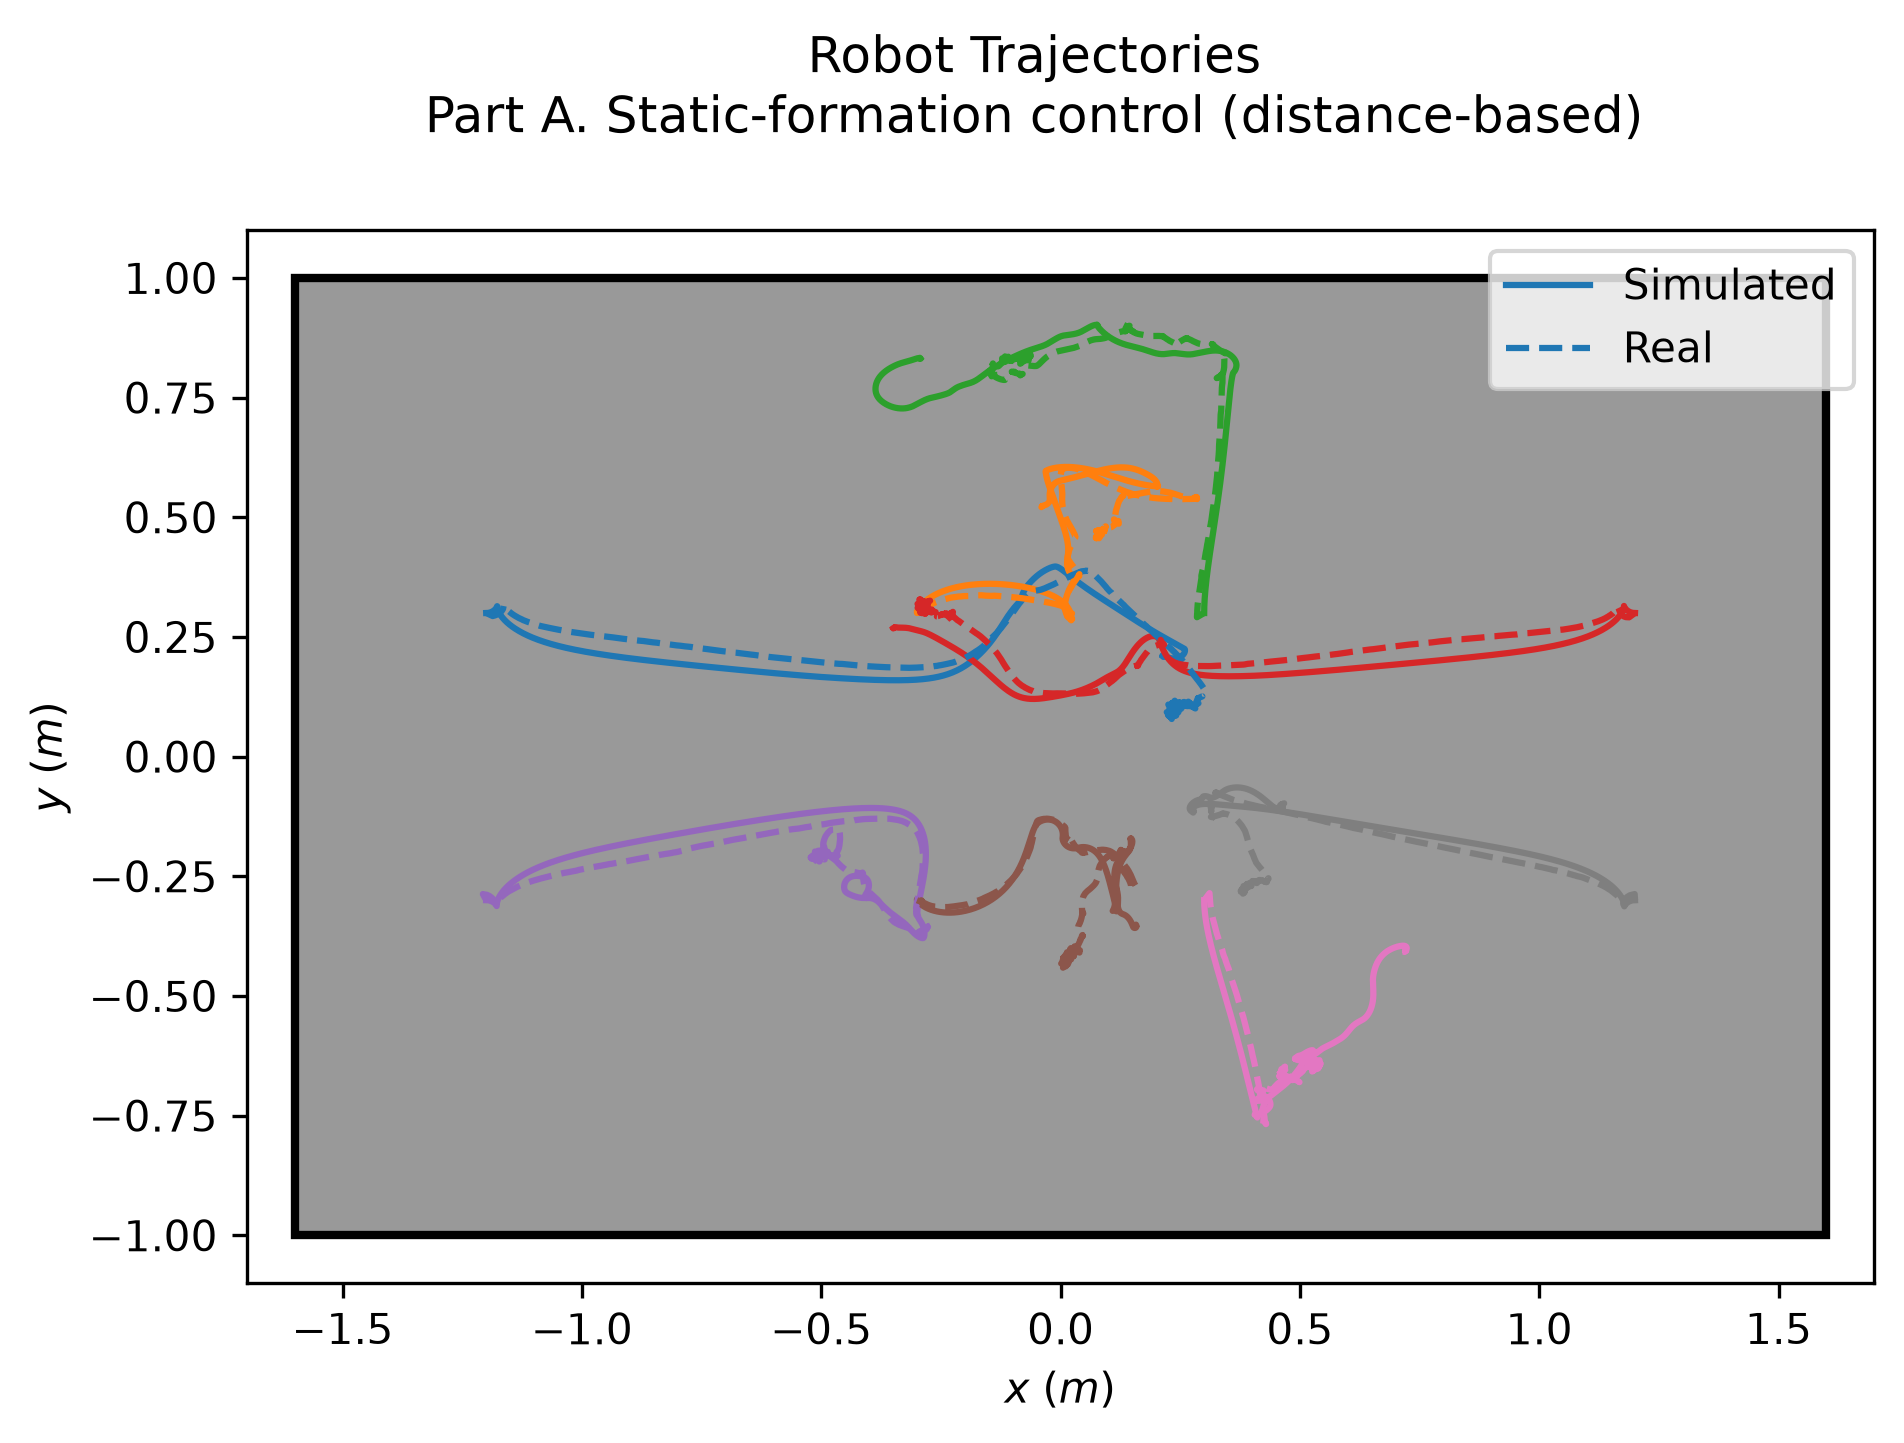
\includegraphics[width=\textwidth]{Figures/a_traj_dist.png}
        \captionsetup{justification=centering}
        \caption{Simulation and hardware robot trajectories for a static formation with distance-based control.}
        % \label{fig:}
    \end{subfigure}\hfill
    \begin{subfigure}[t]{0.45\textwidth}
        \centering
        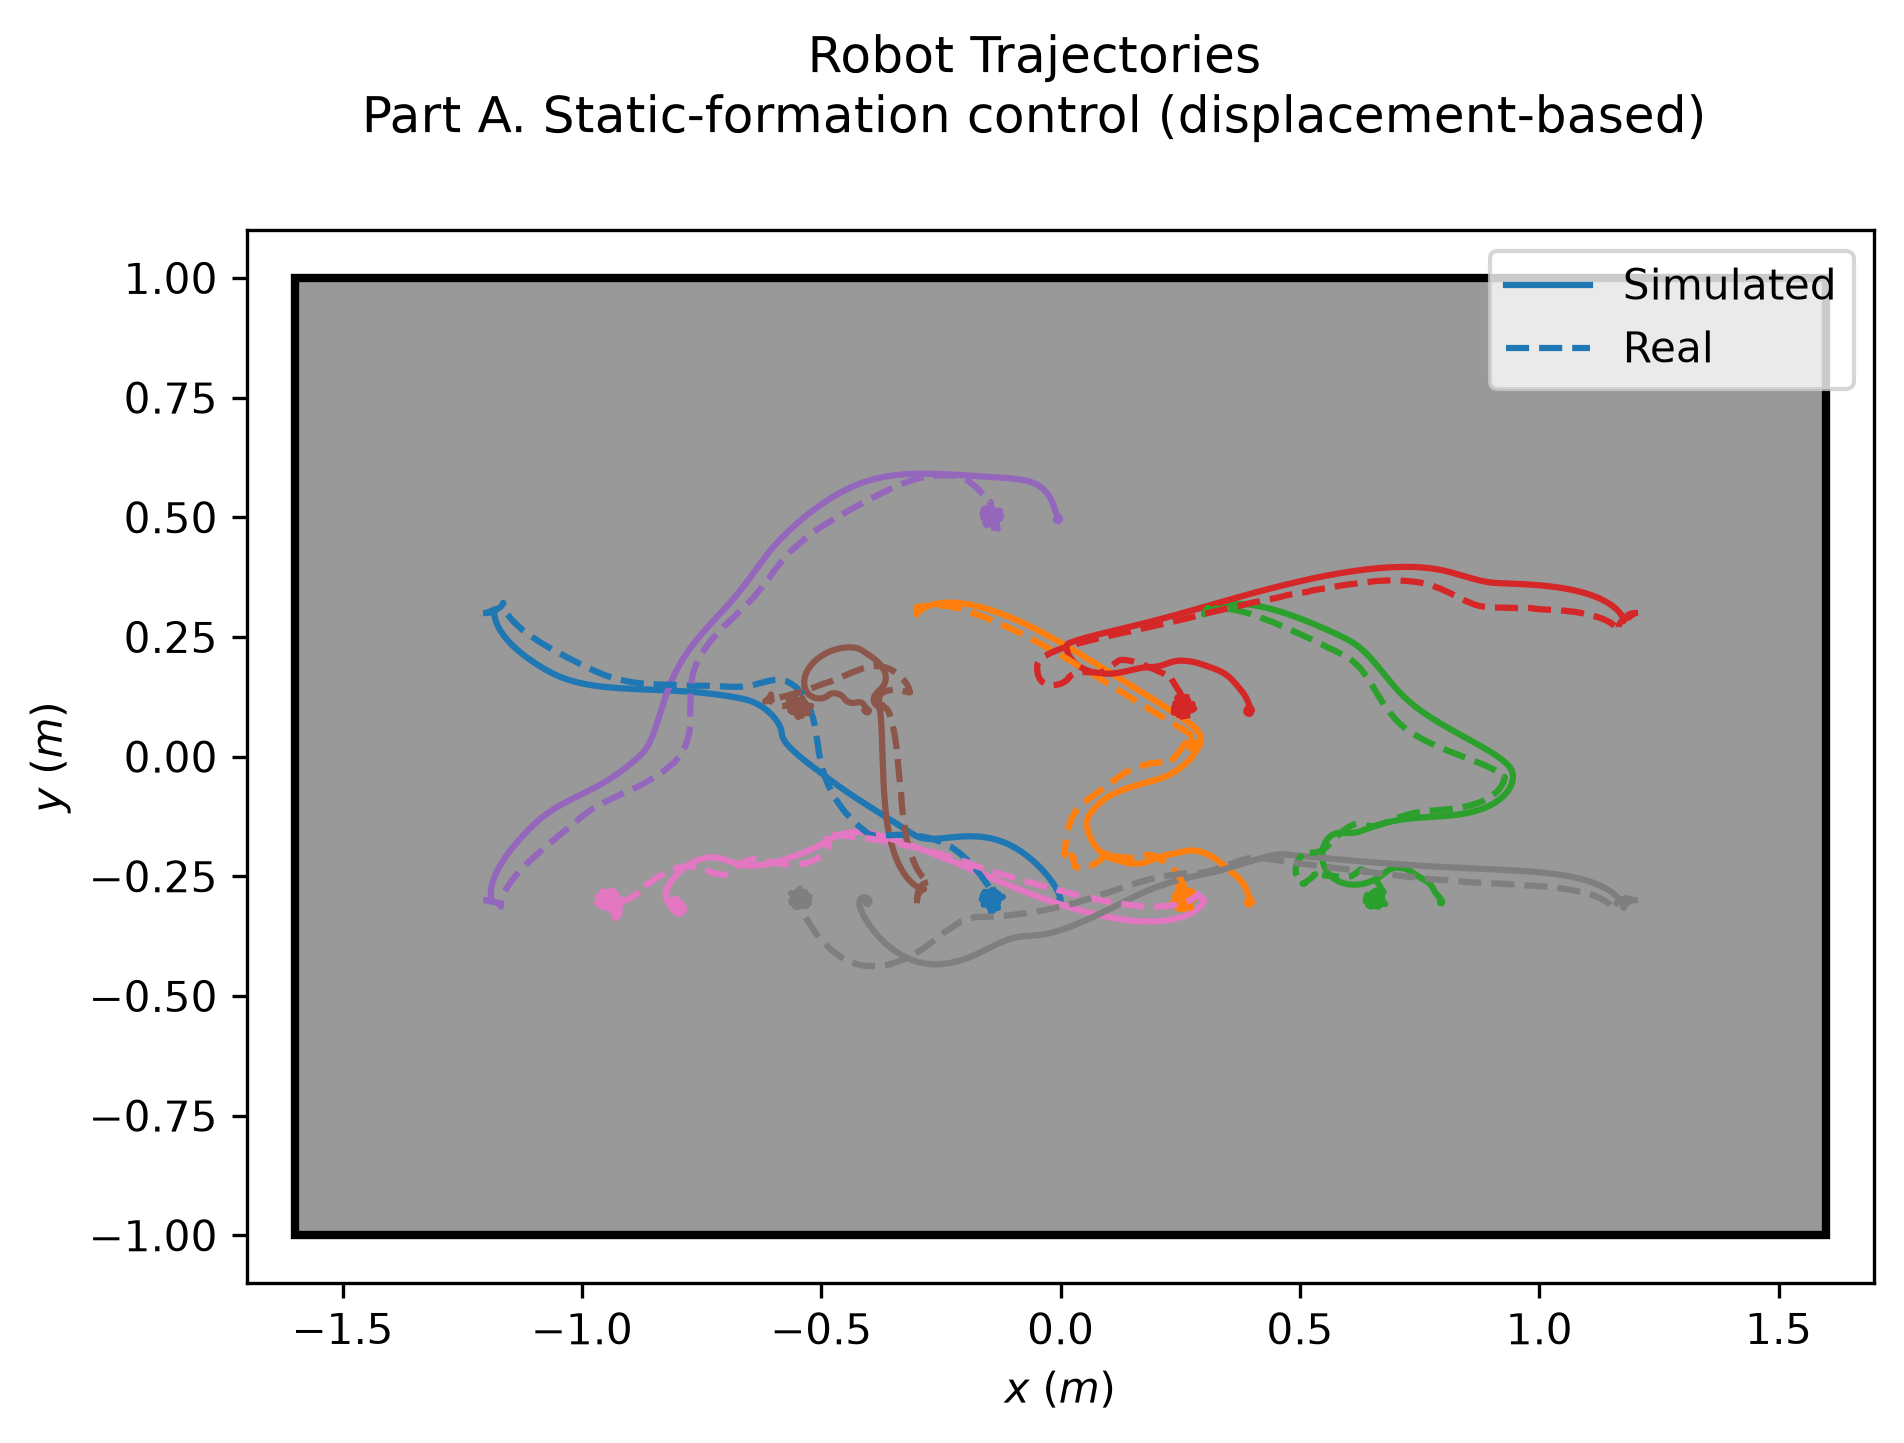
\includegraphics[width=\textwidth]{Figures/a_traj_disp.png}
        \captionsetup{justification=centering}
        \caption{Simulation and hardware robot trajectories for a static formation with displacement-based control.}
        % \label{fig:}
    \end{subfigure}
    \captionsetup{justification=centering}
    \caption{Static-formation control simulation and hardware robot trajectories.}
    \label{fig:traj_a}
\end{figure}

To better visualize the performance of the algorithms in matching the correct graph formation in (\ref{eqn:graph_ac}), the distance constraint error was plotted for both the simulation and hardware experiments, given in Figure \ref{fig:dist_a}. As seen, when \textit{only} considering the distance constraints (and not global translations or rotations of the formation), the distance constraint errors both reached $\sim0$, signifying a success. While perhaps the displacement-based algorithm was slightly more efficient, reaching the correct formation in $\sim25\ s$ compared to the distance-based algorithm in $\sim28\ s$, there is no conclusive advantage for either strategy. However, as will be seen in Part C. the distance-based algorithm only converged because of the \textit{addition} of the extra communication edge between robots 2 and 6. Without that edge, the distance-based controller fails from identical initial conditions, while the displacement-based controller succeeds. Because of this, for graphs with limited communication (or \textit{minimally} rigid), the displacement-based controller may be better, although it limits the flexibility of the formation to be formed at arbitrary orientations.

\begin{figure}[htb]
    \centering
    \begin{subfigure}[t]{0.45\textwidth}
        \centering
        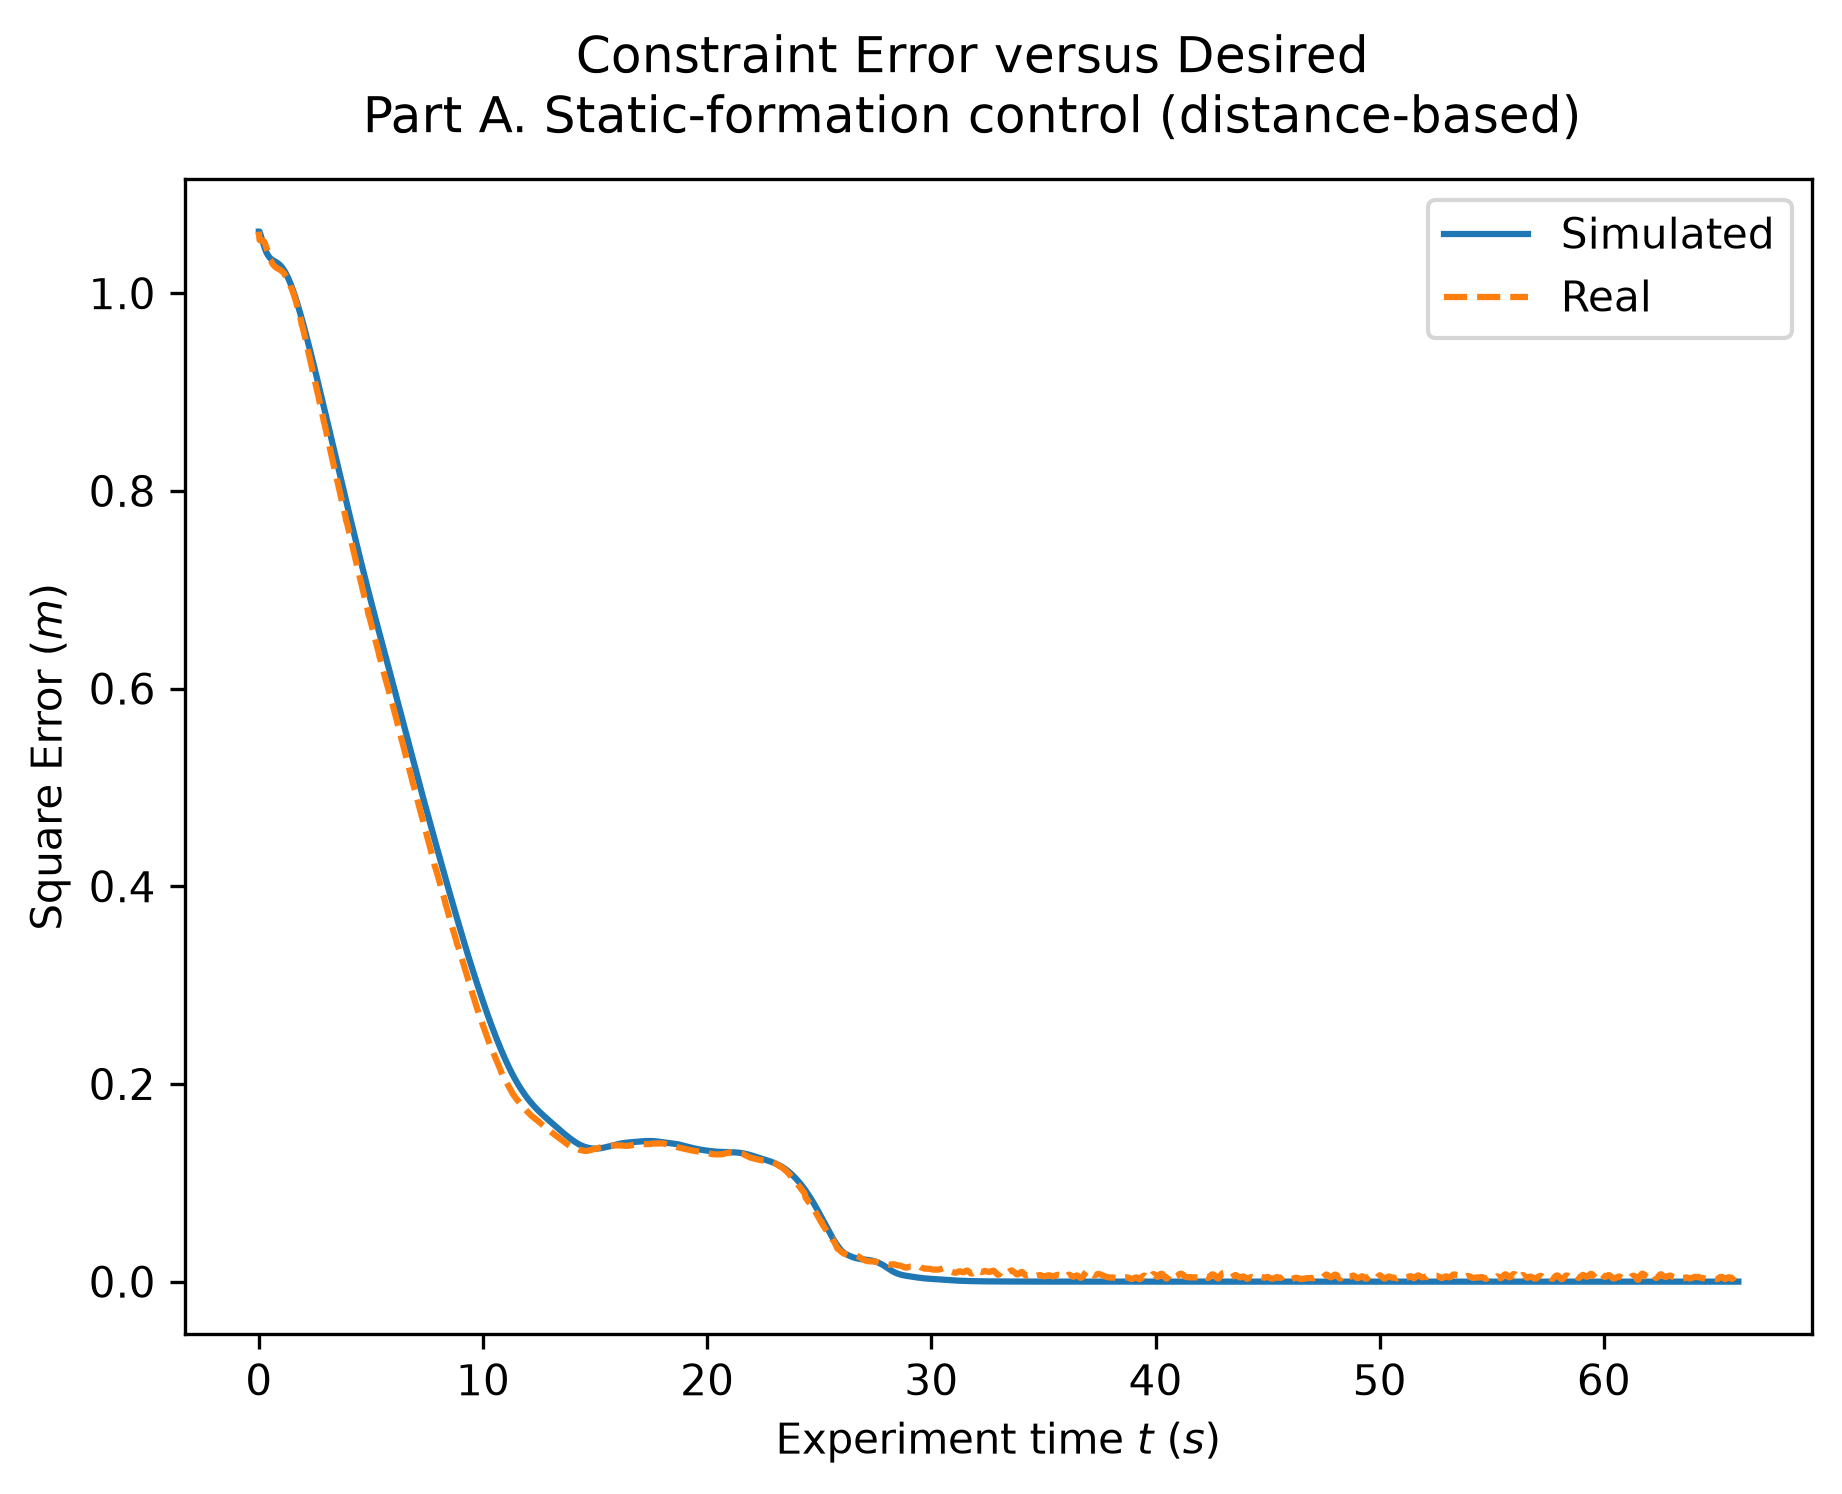
\includegraphics[width=\textwidth]{Figures/a_dist_const_error.png}
        \captionsetup{justification=centering}
        \caption{Simulation and hardware distance constraint error for a static formation with distance-based control.}
        % \label{fig:}
    \end{subfigure}\hfill
    \begin{subfigure}[t]{0.45\textwidth}
        \centering
        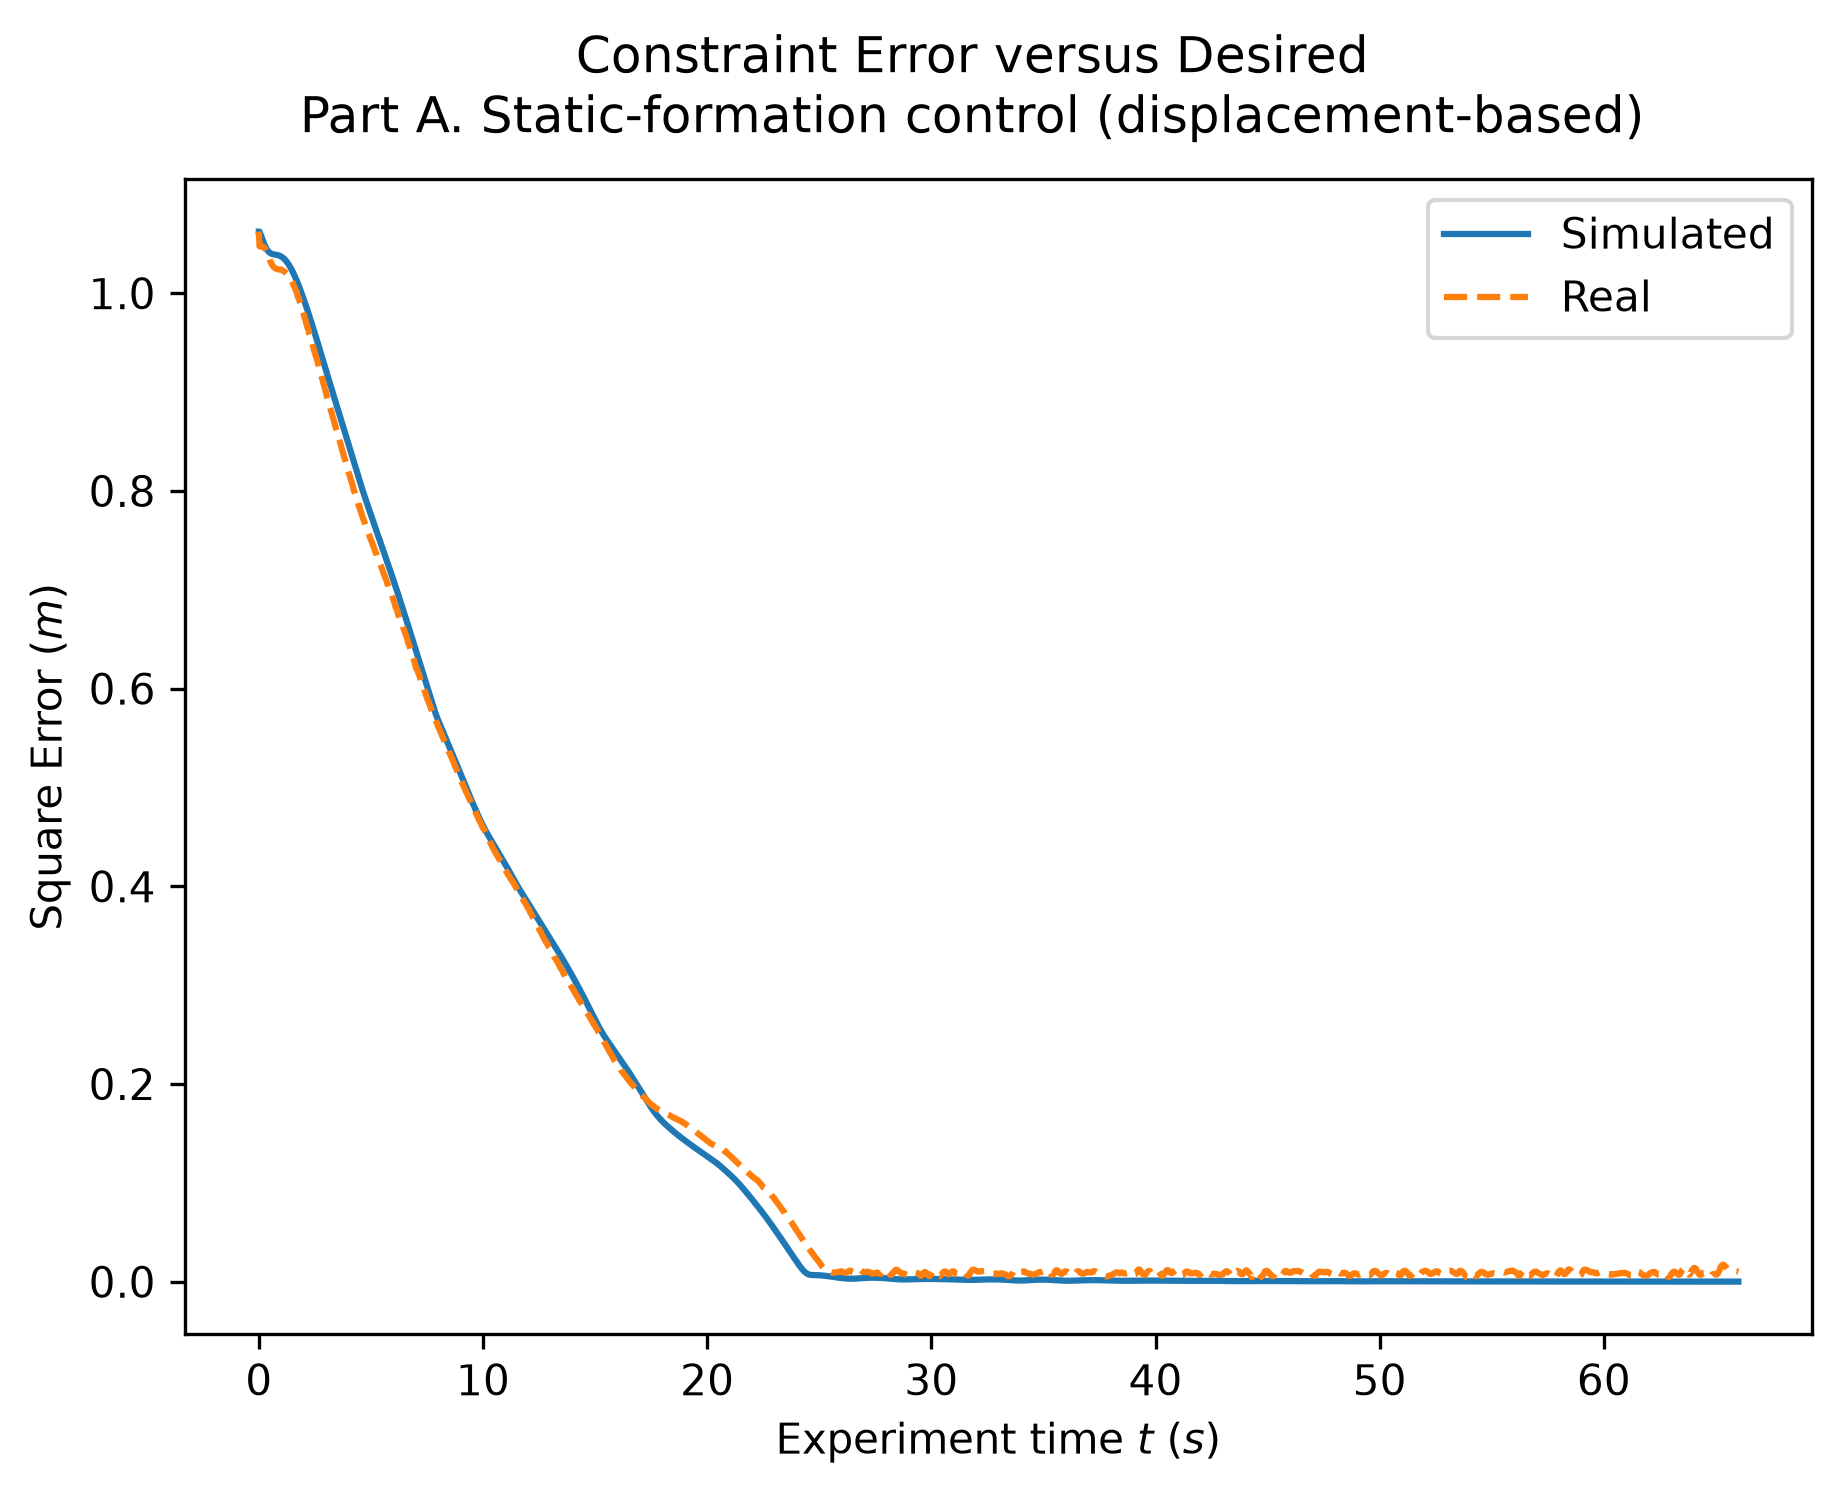
\includegraphics[width=\textwidth]{Figures/a_disp_const_error.png}
        \captionsetup{justification=centering}
        \caption{Simulation and hardware distance constraint error for a static formation with displacement-based control.}
        % \label{fig:}
    \end{subfigure}
    \captionsetup{justification=centering}
    \caption{Static-formation control simulation and hardware distance constraint errors.}
    \label{fig:dist_a}
\end{figure}

\FloatBarrier
As seen in Figures \ref{fig:traj_a} and \ref{fig:dist_a}, visually, both the simulated results and hardware results matched very closely. To better gauge this, the squared error between the simulated poses $p^{real}(t)$ and simulated poses $p^{sim}(t)$ was calculated for both algorithms and given in Figure \ref{fig:square_a}. As seen, for both cases, the error between the simulation and the hardware grew as the experiment continued, up until the final formations were formed, when the error ``leveled off''. This is not surprising, as the simulation is simply an approximation of the real robots, and while it may be high fidelity, any minor discrepancy between what happens in the real dynamics (wheel slippage, strange friction, air resistance, etc.) will cause deviations to compound the longer the experiment runs. In this case, the displacement-based method was able to achieve a slightly lower squared error than the distance-based method, which can be explained by the lack of the rotational degree of freedom in the final formation.

\begin{figure}[htb]
    \centering
    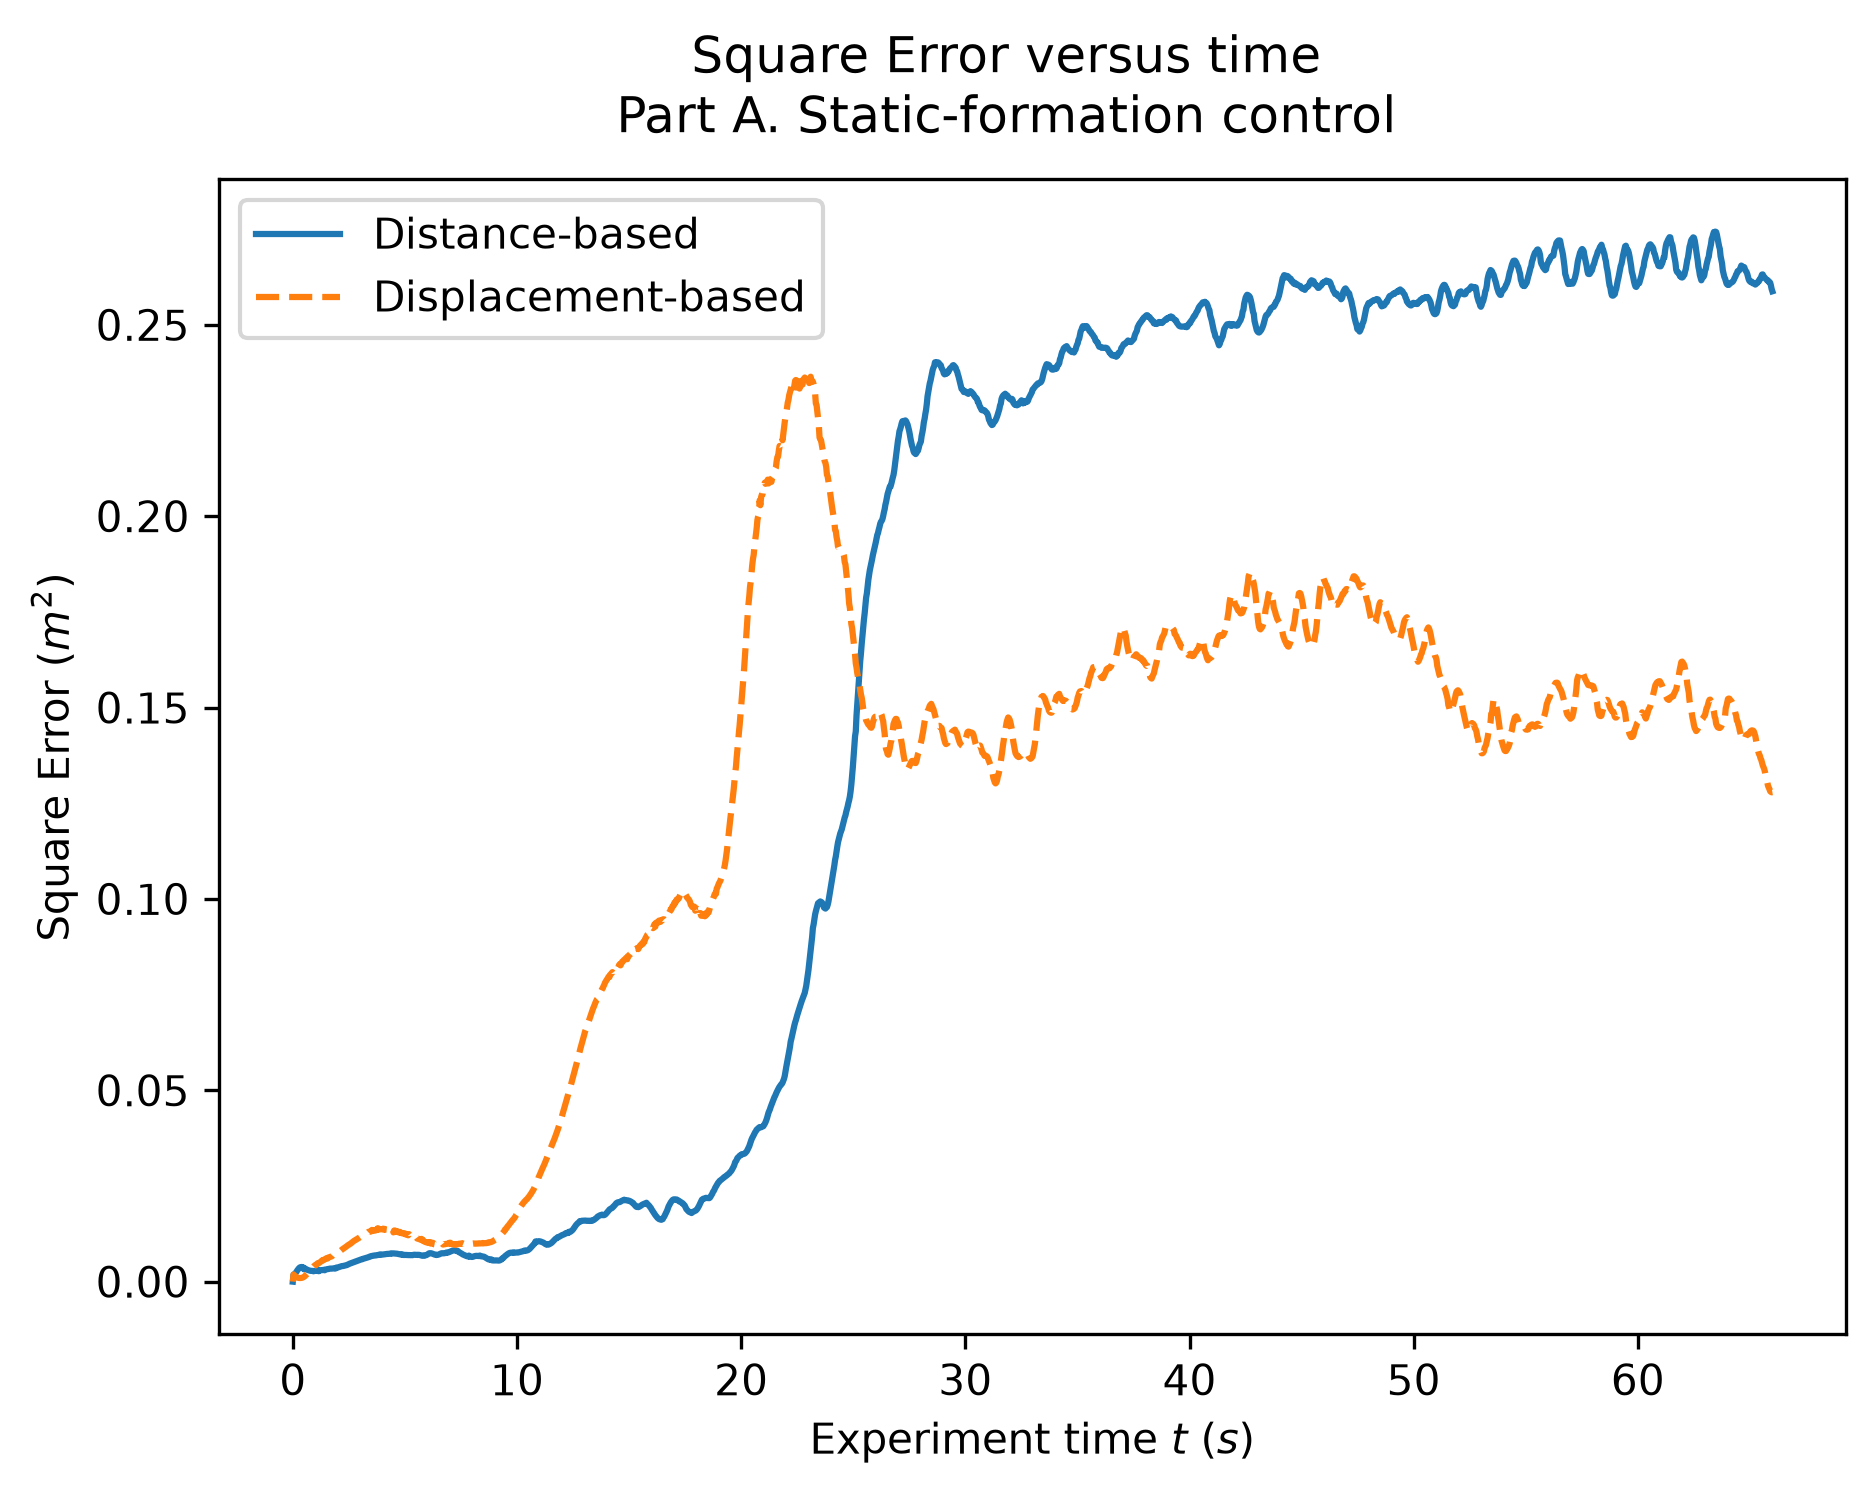
\includegraphics[width=0.5\textwidth]{Figures/a_square_error.png}
    \captionsetup{justification=centering}
    \caption{Square error between $p^{real}(t)$ and $p^{sim}(t)$ for both distance-based and displacement-based controllers.}
    \label{fig:square_a}
\end{figure}

\clearpage
\subsection*{B. Track a moving reference}
\subsubsection*{1.}
Define a set of 3--6 waypoints in the arena for the group to visit (see \texttt{leader\_follower} example for a four-waypoint implementation; you may keep these waypoints or design your own sequence). Plot the location of these waypoints on the arena map.

\subsubsection*{ANSWER:}
For the moving reference formation control, 4 waypoints $w$ were chosen similarly to what was provided in the \texttt{leader\_follower} example, with coordinates (in meters $m$)
\begin{align*}
    w_1&=(-1,0.5) & w_2&=(-1,-0.5) & w_3&=(1,-0.5) & w_4&=(1,0.5)\,.
\end{align*}
These waypoints can be seen in the trajectory plots in Figures \ref{fig:traj_dist_global_b} and \ref{fig:traj_leader_b}.

For the following experiments, because of space constraints in the arena, a formation and graph $\mathcal G_b=(\mathcal V_b,\mathcal E_b)$ was constructed so that the robots would have more room to maneuver while following the reference/leader. The new pairwise distance constraints are
\begin{align}\label{eqn:graph_b}
    d_{ij}^b&=\begin{pmatrix}
        0 & 0.6 & 0.6\sqrt 2 & 0.6\\
        0.6 & 0 & 0.6 & 0.6\sqrt 2\\
        0.6\sqrt 2 & 0.6 & 0 & 0.6\\
        0.6 & 0.6\sqrt 2 & 0.6 & 0
    \end{pmatrix}\,,
\end{align}
which is a fully-connected graph that creates a formation of a square with side-length $0.6\ m$ with robot coordinates relative to the reference point of (in meters $m$)
\begin{align}\label{eqn:p_b}
    p_1&=(-0.3,0.3) & p_2&=(0.3,0.3) & p_3&=(0.3,-0.3) & p_4&=(-0.3,-0.3)\,.
\end{align}

\FloatBarrier
\subsubsection*{2.}
First, we will have the formation visit the waypoints you define in part 1 with global knowledge of the motion plan. Modify your displacement-based controller from Part A so that the formation reference point moves toward the current waypoint while the robots maintain their desired relative displacements. You can use the leader controller and waypoint-switching logic from the \texttt{leader\_follower} example as a skeleton for the motion plan of the formation reference. Assume that all robots have access to the motion plan.

Run the controller in simulation and in hardware from shared initial conditions. Plot the robot trajectories, $E_d(t)$, and $E_{sim}(t)$ as in Part A. Also plot the squared distance between the formation center and the current waypoint,
\begin{align*}
    E_c(t)&=\|p(t)-w_k(t)\|^2\,,
\end{align*}
for both runs. You may want to save the active-waypoint index along with the position data in your code. How well does the group preserve its shape while moving between waypoints?

\subsubsection*{ANSWER:}
For the global-knowledge case of tracking a moving reference in formation (\ref{eqn:graph_b}) with relative displacements in (\ref{eqn:p_b}), the experiment was run in both simulation and hardware, with the final trajectories given in Figure \ref{fig:traj_dist_global_b}. As seen (considering only global-knowledge in the Figure), the simulation and hardware followed nearly the exact same trajectory with little deviation, which is corroborated by looking at the square error between the simulation and the hardware experiment in Figure \ref{fig:square_way_b}. For this this method, in both cases, between waypoints, the formation preserves its shape very well (especially after $\sim20\ s$), as seen by the near-zero distance constraint error. Perhaps this is not surprising, as once each robot is in the correct place relative to the moving reference, so long as the reference does not move more quickly than the robots can, they should be able to hold their steady position relative to it.

\begin{figure}[htb]
    \centering
    \begin{subfigure}[t]{0.45\textwidth}
        \centering
        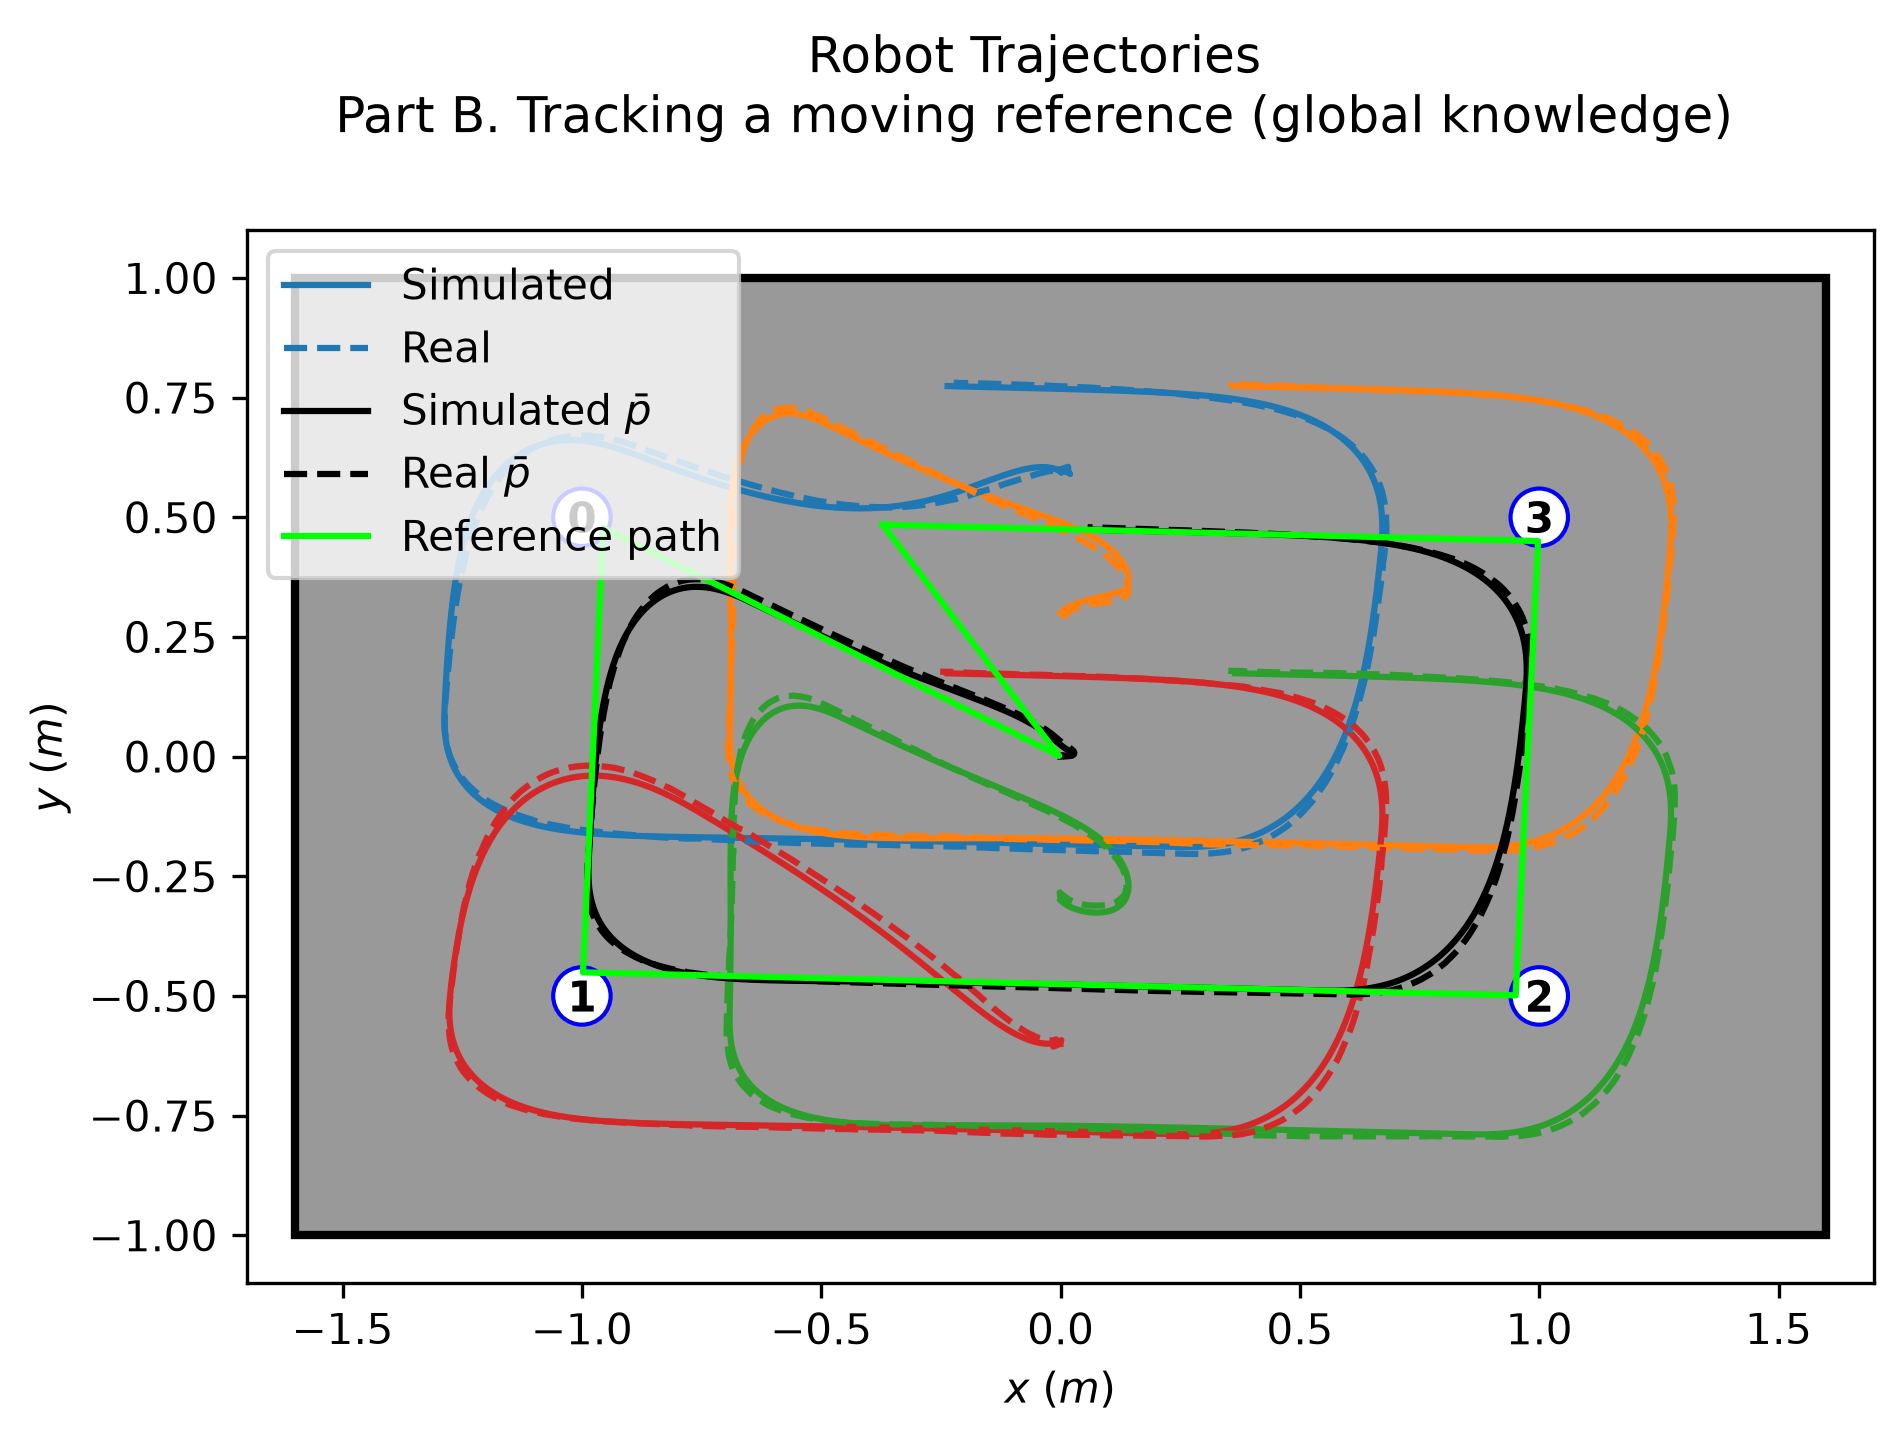
\includegraphics[width=\textwidth]{Figures/b_traj_global.png}
        \captionsetup{justification=centering}
        \caption{Simulation and hardware robot trajectories for global-knowledge formation control with moving reference.}
        % \label{fig:}
    \end{subfigure}\hfill
    \begin{subfigure}[t]{0.45\textwidth}
        \centering
        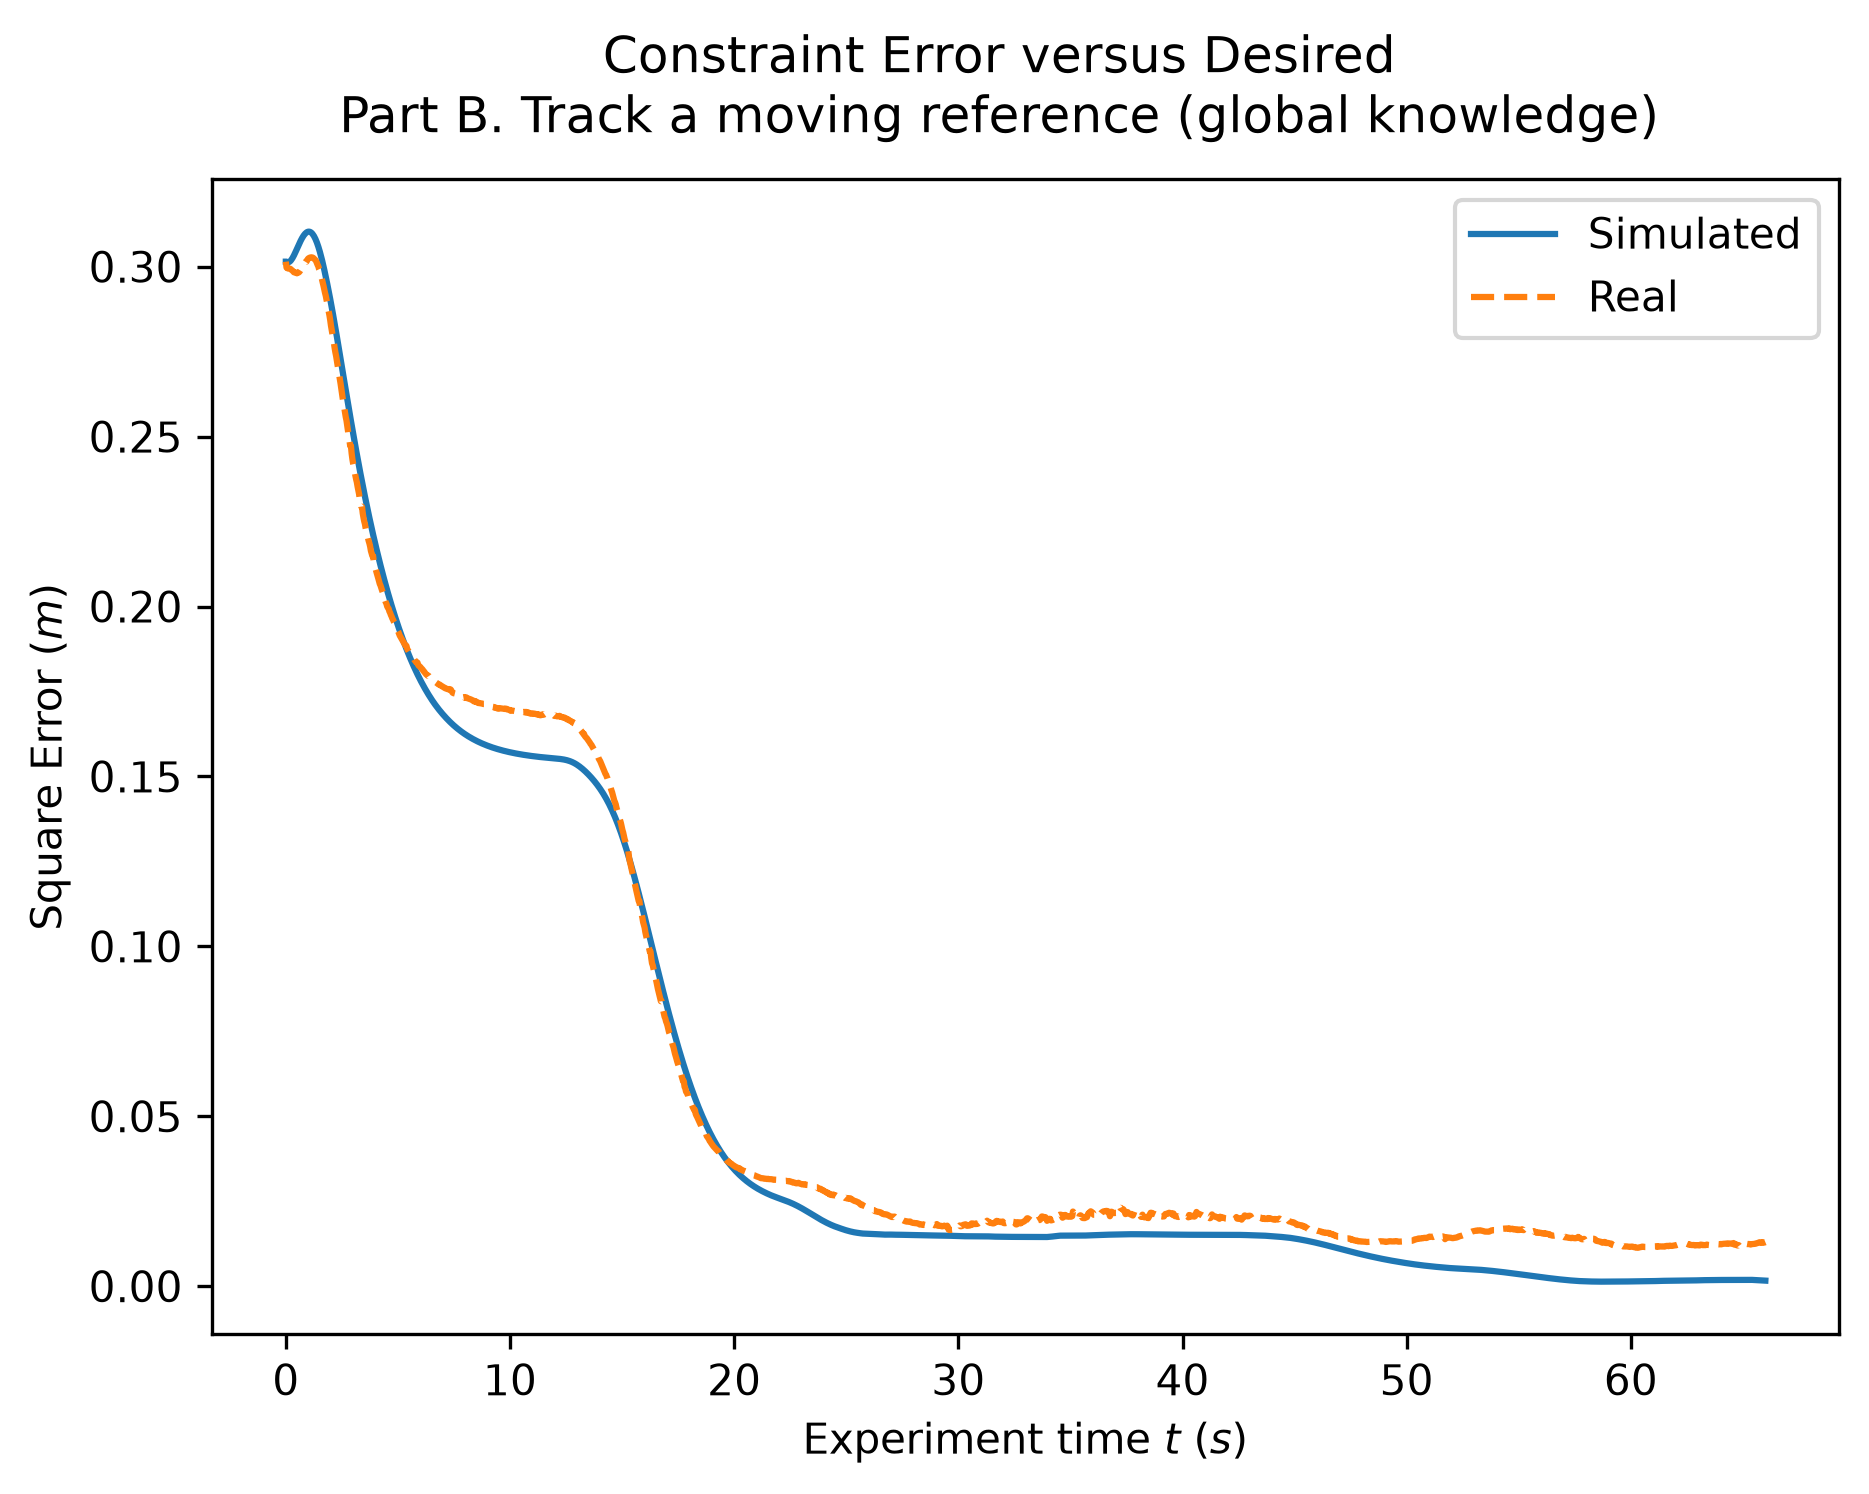
\includegraphics[width=\textwidth]{Figures/b_global_const_error.png}
        \captionsetup{justification=centering}
        \caption{Simulation and hardware distance constraint error for global-knowledge formation control with moving reference.}
        % \label{fig:}
    \end{subfigure}
    \captionsetup{justification=centering}
    \caption{Moving reference global-knowledge formation control trajectories and distance constraint error.}
    \label{fig:traj_dist_global_b}
\end{figure}

The waypoint switching was triggered when the average position of the formation, denoted by $\bar p$, came within a certain tolerance of the current waypoint coordinates. For this experiment, the tolerance was set as $\epsilon=0.05\ m$, and the resulting square error between the simulated/hardware average position and current waypoint is given in Figure \ref{fig:square_way_b}. As seen, when the waypoint switches coordinates (observable by the sharp vertical discontinuity in the error), the square error between the average positon and the new coordinates experiences a large and sudden ``jump''. This is not surprising, as it is this new increase in error that causes the formation, which is following the reference trajectory, to move to the next waypoint reference. But, as seen in Figure \ref{fig:traj_dist_global_b}, this sharp increase in error does \textit{not} affect the formation's ability to maintain its shape, as the shape is defined only according to the moving reference, not the current waypoint.

\begin{figure}[htb]
    \centering
    \begin{subfigure}[t]{0.45\textwidth}
        \centering
        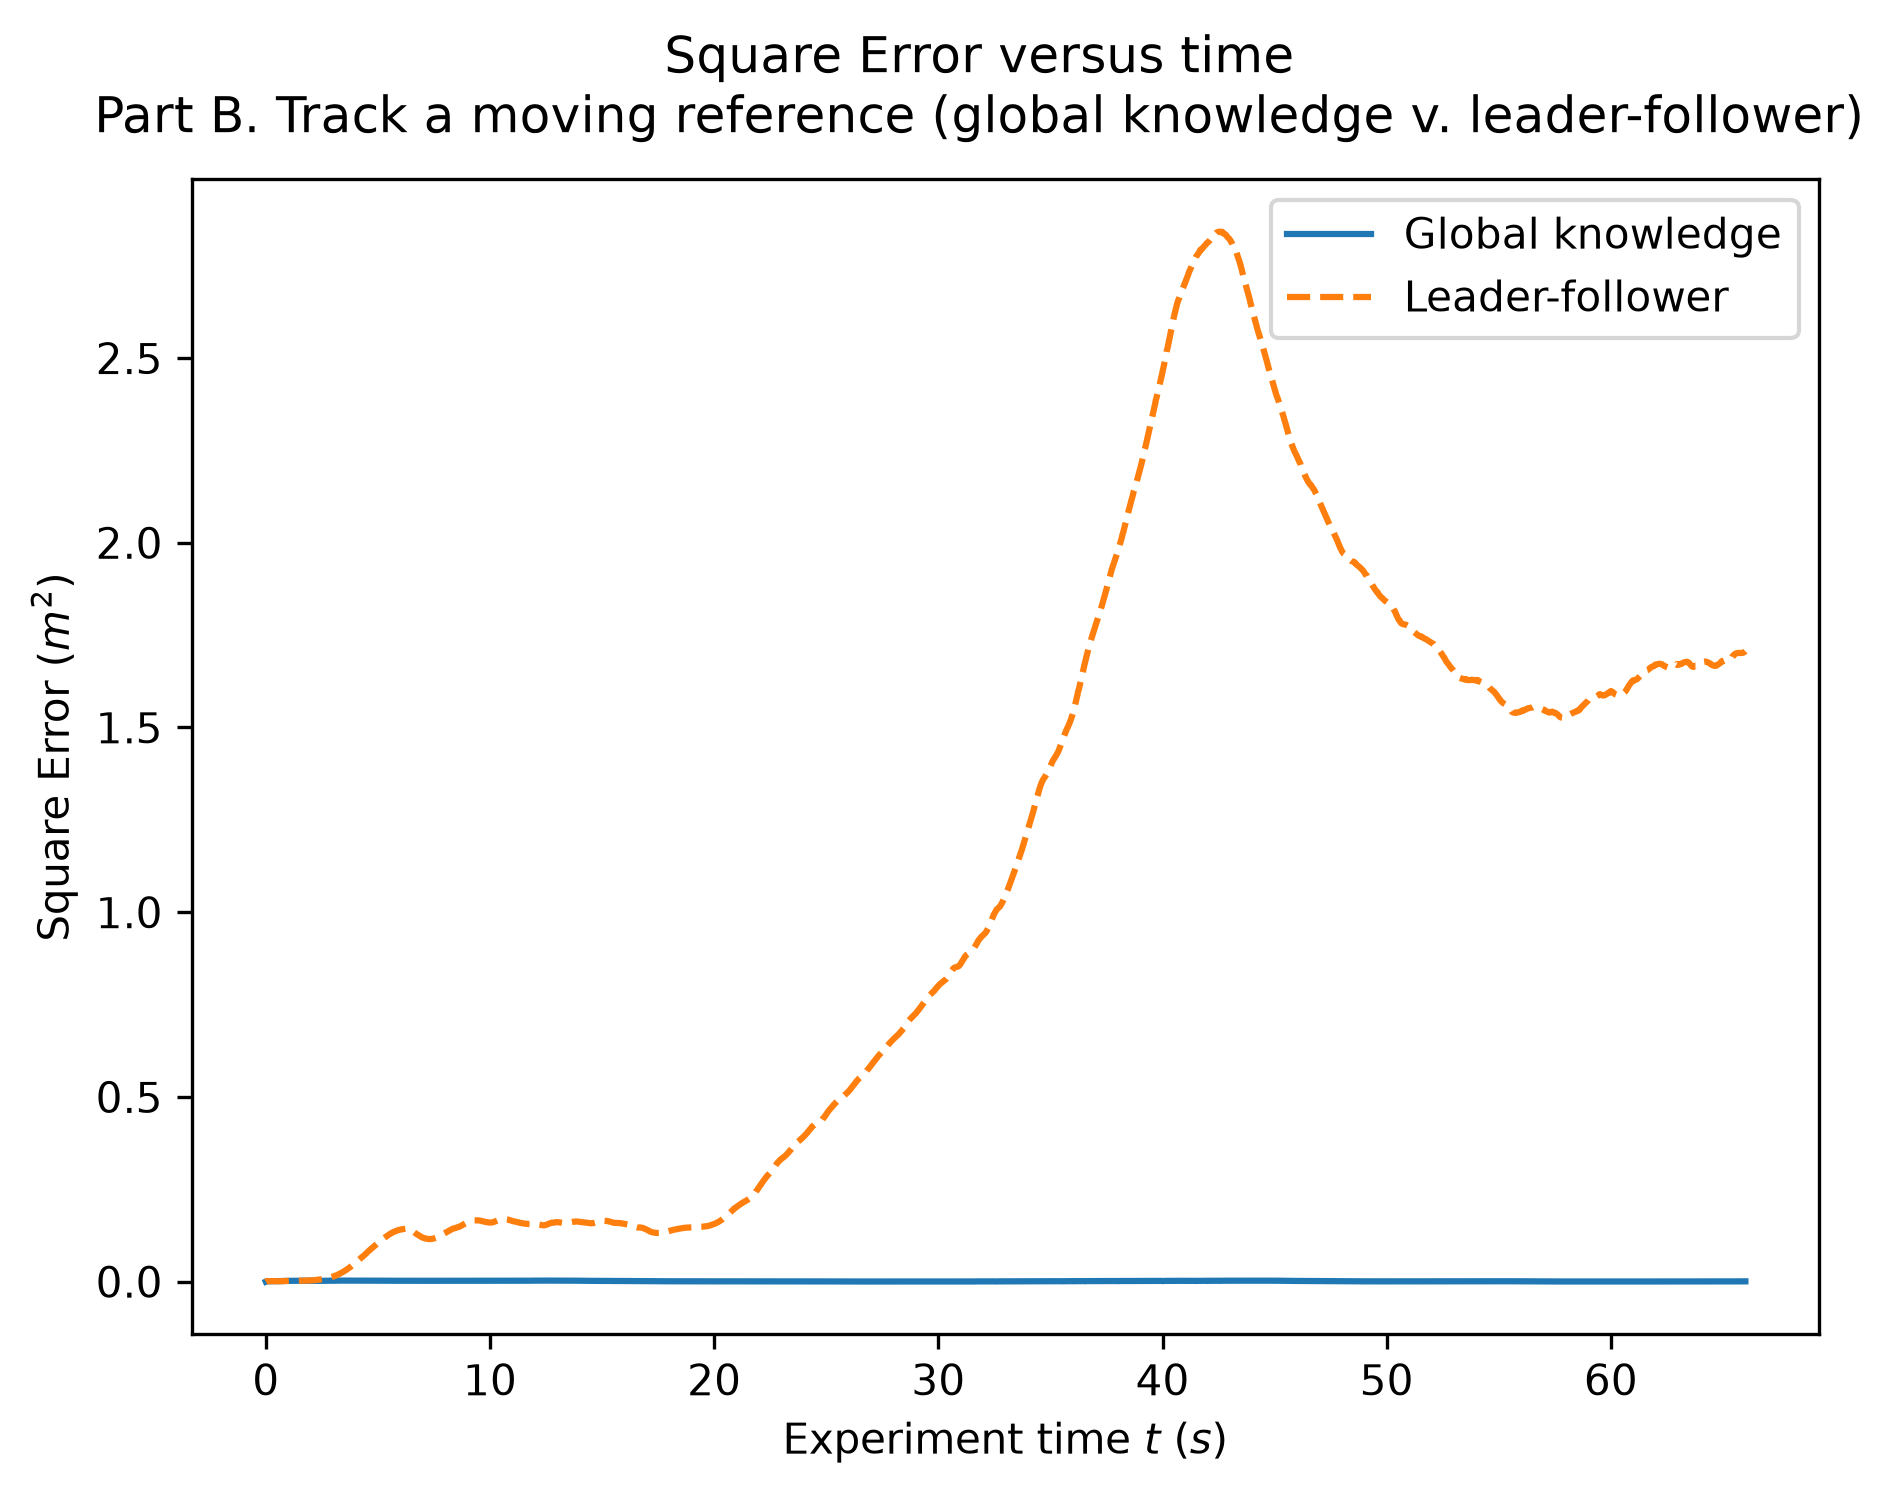
\includegraphics[width=\textwidth]{Figures/b_square_error.png}
        \captionsetup{justification=centering}
        \caption{Square error between $p^{real}(t)$ and $p^{sim}(t)$ for both global-knowledge and leader-follower moving reference formation control.}
        % \label{fig:}
    \end{subfigure}\hfill
    \begin{subfigure}[t]{0.45\textwidth}
        \centering
        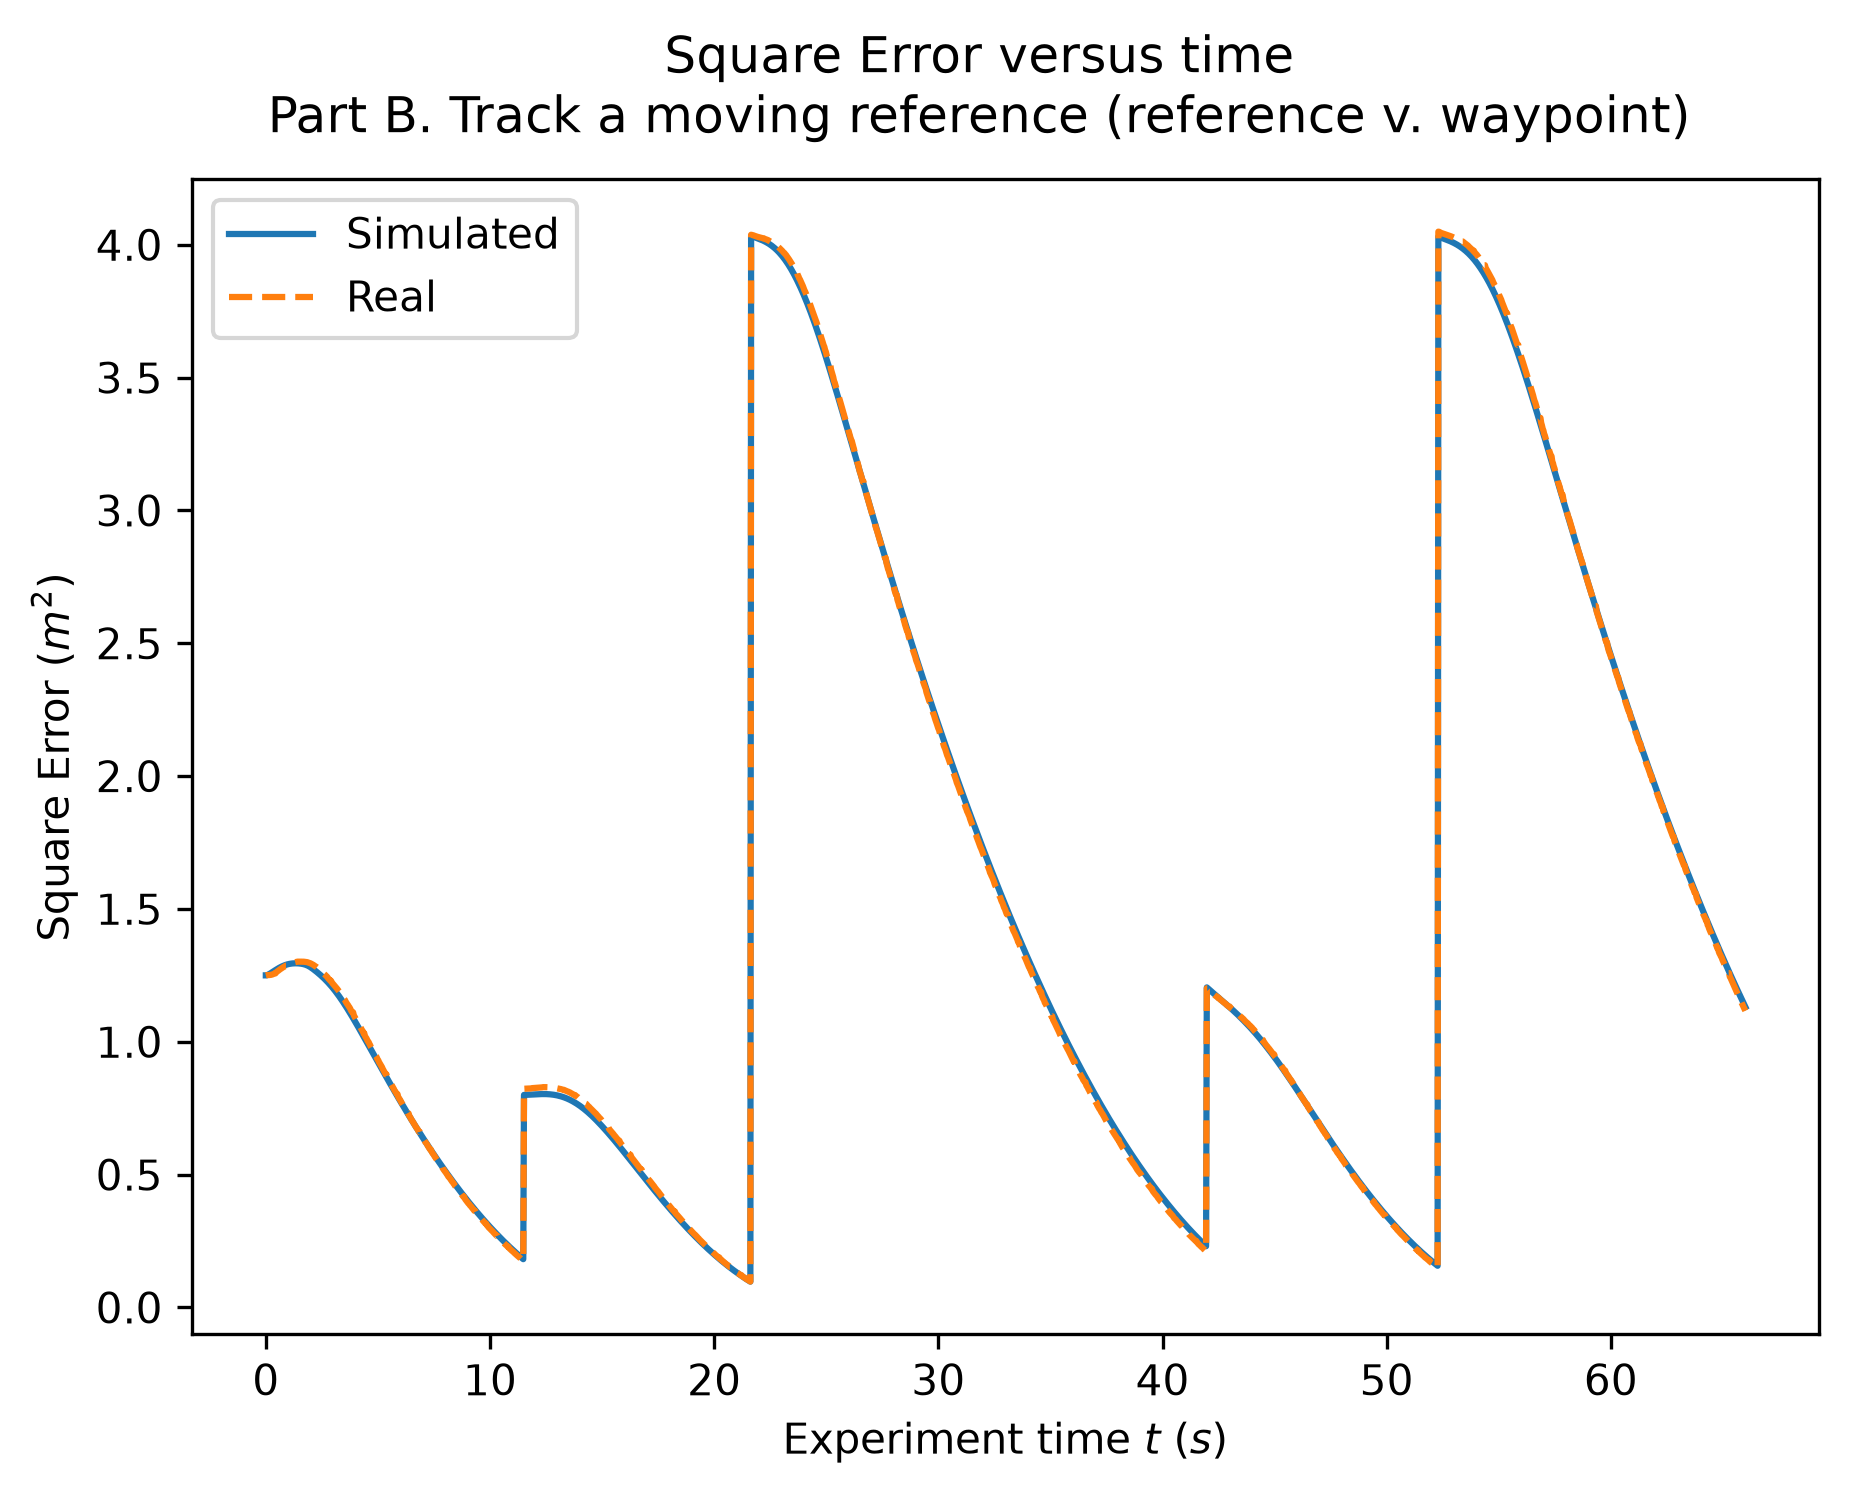
\includegraphics[width=\textwidth]{Figures/b_reference_error.png}
        \captionsetup{justification=centering}
        \caption{Square error between $\bar p(t)$ and the current waypoint coordinate $w_k(t)$ for global-knowledge moving reference formation control.}
        % \label{fig:}
    \end{subfigure}
    \captionsetup{justification=centering}
    \caption{Moving reference formation control, square error (global-knowledge and leader-follower) and waypoint reference square error (global-knowledge).}
    \label{fig:square_way_b}
\end{figure}

\FloatBarrier
\subsubsection*{3.}
Next, we will assume only one robot has access to the motion plan. Modify your distance-based controller from Part A and add a separate robot as a leader (your group will now be $N+1$). Use the leader controller and waypoint-switching logic from the \texttt{leader\_follower} example to move the leader through the same waypoint sequence.

Choose one or more formation members to receive the leader's measured position, and add distance constraints between these robots and the leader. Choose these distances to be consistent with a desired location of the leader relative to your formation.

Run this strategy in simulation and in hardware from shared initial conditions, using the same initial poses for the formation members as in item 2. Plot the leader and follower trajectories and $E_{sim}(t)$ for the formation members. Plot the distance constraint error separately for the original formation edges and the added leader-follower edges, using the definition of $E_d(t)$ for each edge set. How effectively does the formation follow the leader? How does the resulting movement compare to (e.g., how well is the shape and orientation preserved during movement?) what happens when you switch from one waypoint to the next?

\subsubsection*{ANSWER:}
A designated leader was added to the formation in (\ref{eqn:p_b}) such that the leader's coordinates in the square formation were the center, so the distance constraints in (\ref{eqn:graph_b}) became
\begin{align}\label{eqn:graph_b_l}
    p_\ell&=(0,0) & d_{ij}'^b&=\begin{pmatrix}
        0 & 0.3\sqrt 2 & 0.3\sqrt 2 & 0.3\sqrt 2 & 0.3\sqrt 2\\
        0.3\sqrt 2 & 0 & 0.6 & 0.6\sqrt 2 & 0.6\\
        0.3\sqrt 2 & 0.6 & 0 & 0.6 & 0.6\sqrt 2\\
        0.3\sqrt 2 & 0.6\sqrt 2 & 0.6 & 0 & 0.6\\
        0.3\sqrt 2 & 0.6 & 0.6\sqrt 2 & 0.6 & 0
    \end{pmatrix}\,,
\end{align}
with new communication graph adjacency given as
\begin{align*}
    A'^b&=\begin{pmatrix}
        0 & 0 & 0 & 0 & 0\\
        1 & 0 & 1 & 1 & 1\\
        0 & 1 & 0 & 1 & 1\\
        1 & 1 & 1 & 0 & 1\\
        0 & 1 & 1 & 1 & 0
    \end{pmatrix}\,,
\end{align*}
showing that only robots 0 and 2 receive information from the leader to maintain the desired formation in (\ref{eqn:graph_b_l}), while the leader receives \textit{no} information from any of the other robots.

With this configuration, the leader was sent to track the same waypoints as in the global-knowledge experiment while the other robots used distance-based algorithms to maintain formation, starting from identical initial conditions. The resulting trajectories from both the simulated and hardware results are provided in Figure \ref{fig:traj_leader_b}. As seen, the two experiments (simulation and hardware) do \textit{not} agree, and while the simulation was able to achieve nearly desired formation, the hardware robots were not. The reason for this is due to the small discrepancies between the simulator and the real physical systems. Slight deviations in the initial behavior, much like chaotic systems, can lead to drastically different outcomes. And while this may not have been the case for an alternate initial configuration, it seems that this state is an unstable configuration, and so the physical results do not agree with simulation. Figure \ref{fig:square_way_b} shows the square error between the leader-follower simulation and hardware, and while it is expected to grow, it is \textit{very} large when compared to the global-knowledge strategy. This suggests that global-knowledge moving reference formation control is more robust with its convergence (at least in the case where limited robots have communication with the leader). If \textit{all} of the robots were able to communicate with the leader, then most likely the formation would have been achieved in both simulation and hardware, but that requires more communication between agents, which may not be acheivable in a real system.

\begin{figure}[htb]
    \centering
    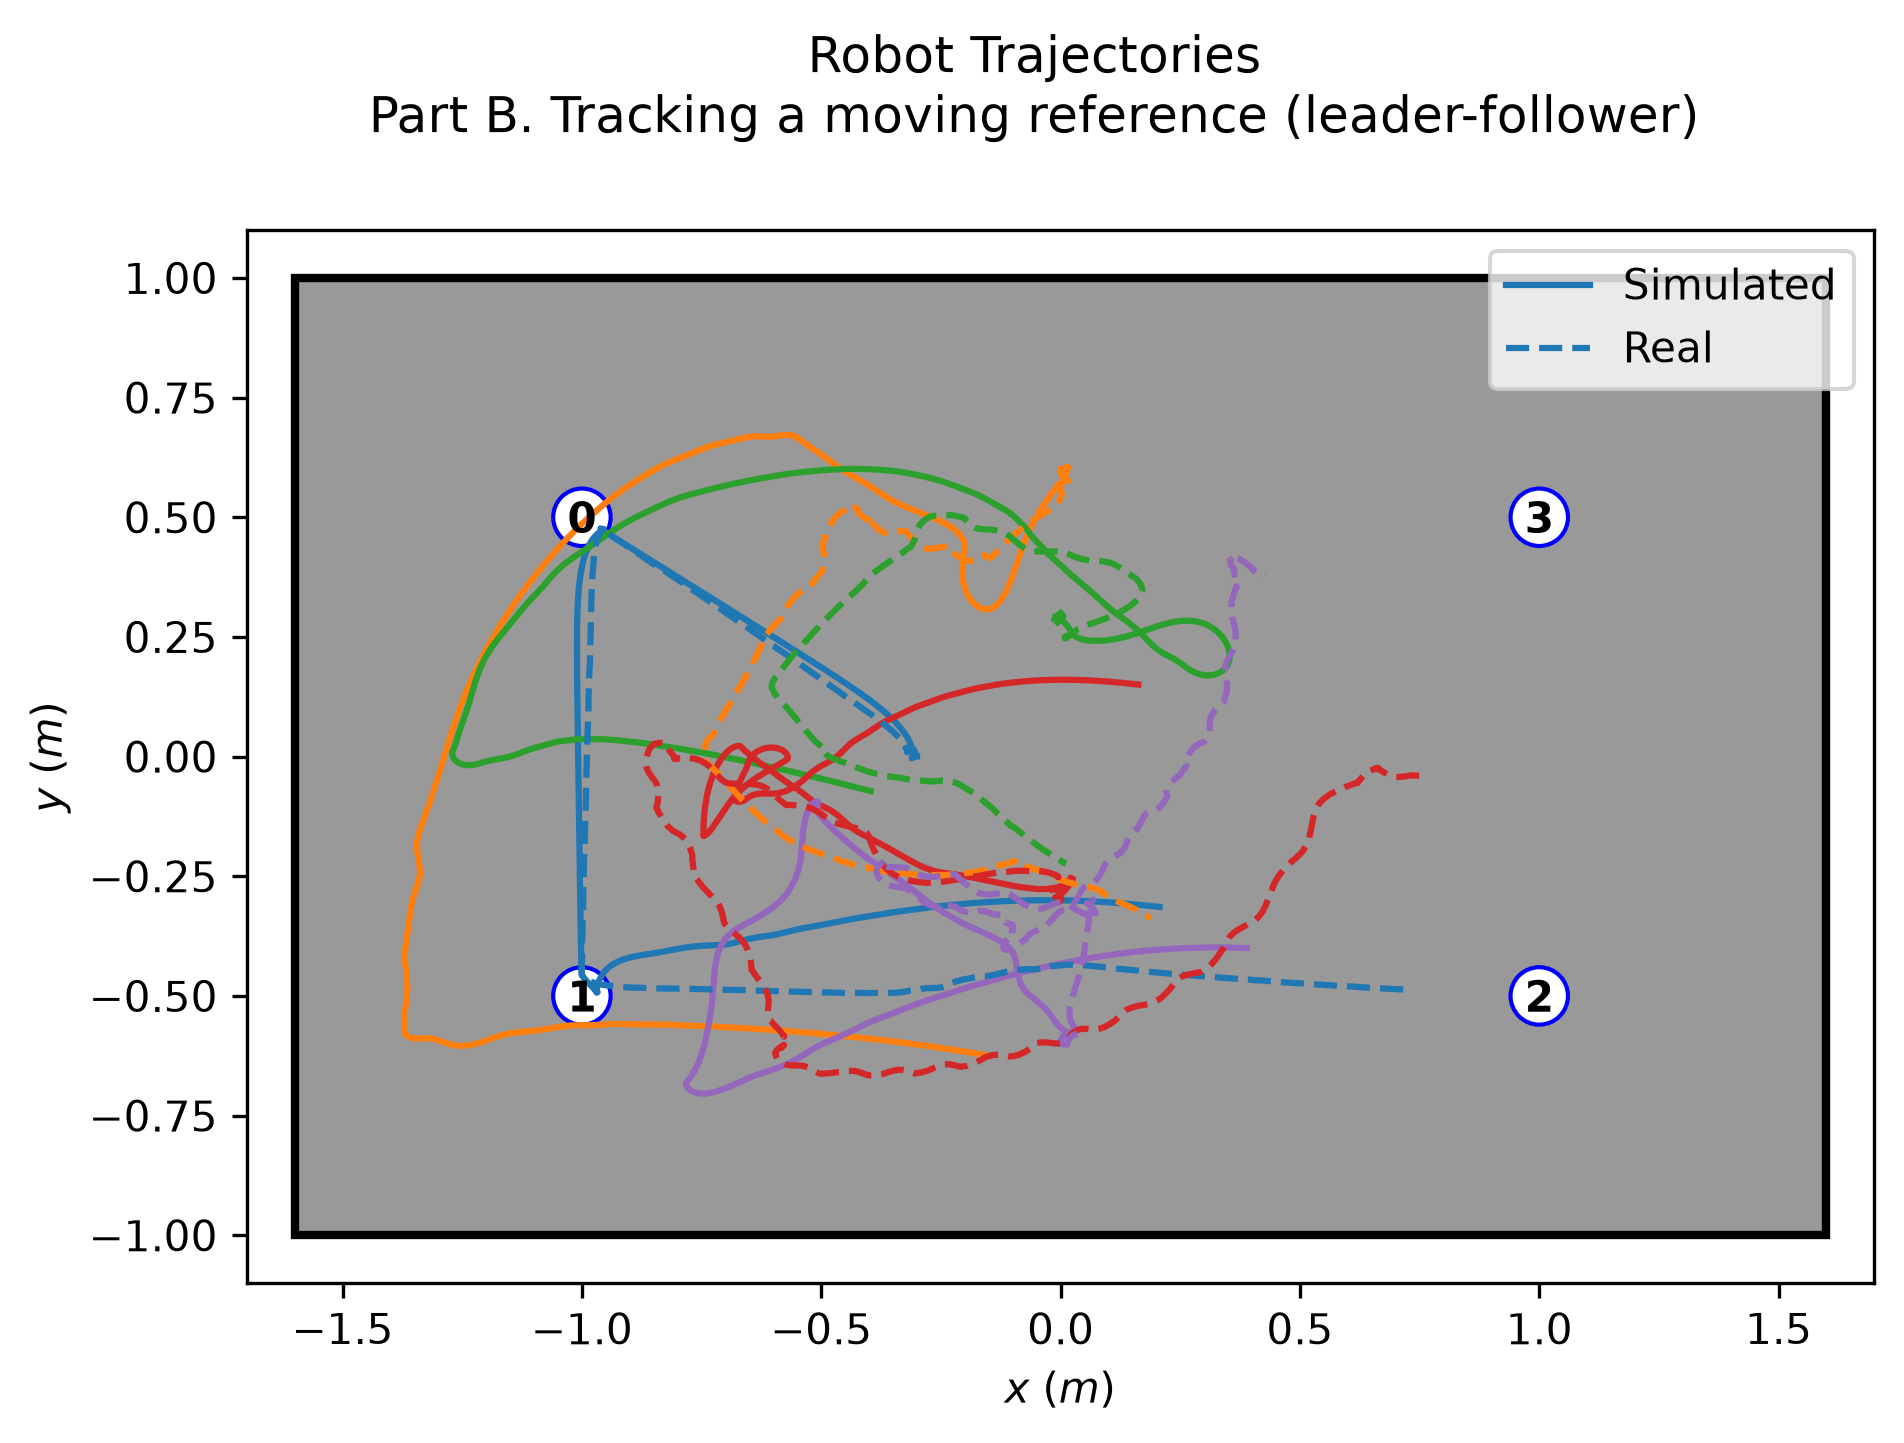
\includegraphics[width=0.5\textwidth]{Figures/b_traj_leader.png}
    \captionsetup{justification=centering}
    \caption{Simulation and hardware robot trajectories for leader-follower formation control with moving reference.}
    \label{fig:traj_leader_b}
\end{figure}

\FloatBarrier
To better illustrate the convergence to the desired formation, the distance constraint error is provided in Figure \ref{fig:dist_b_l} for both the \textit{total} formation and for the follower formation, comparing to (\ref{eqn:graph_b_l}) and (\ref{eqn:graph_b}), respectively. As seen (which may not be obvious when looking at the trajectories in Figure \ref{fig:traj_leader_b}), the simulation does converge towards the desired follower formation, but it is less successful in converging to the formation with the leader. This is because only two of the robots received information from the leader, so while they have maintained proper distance from the leader, the other follower robots did not, and the follower formation could have been rotated and shifted from what was desired. However, the hardware experiment does not converge in either case, and the formation remains far from the desired configuration. Therefore, to improve the results, more robots should receive information from the leader so that they can properly position themselves relative to it, as even if the follower shape is maintained between waypoints, it may not be correctly maintained about the leader's position.

\begin{figure}[htb]
    \centering
    \begin{subfigure}[t]{0.45\textwidth}
        \centering
        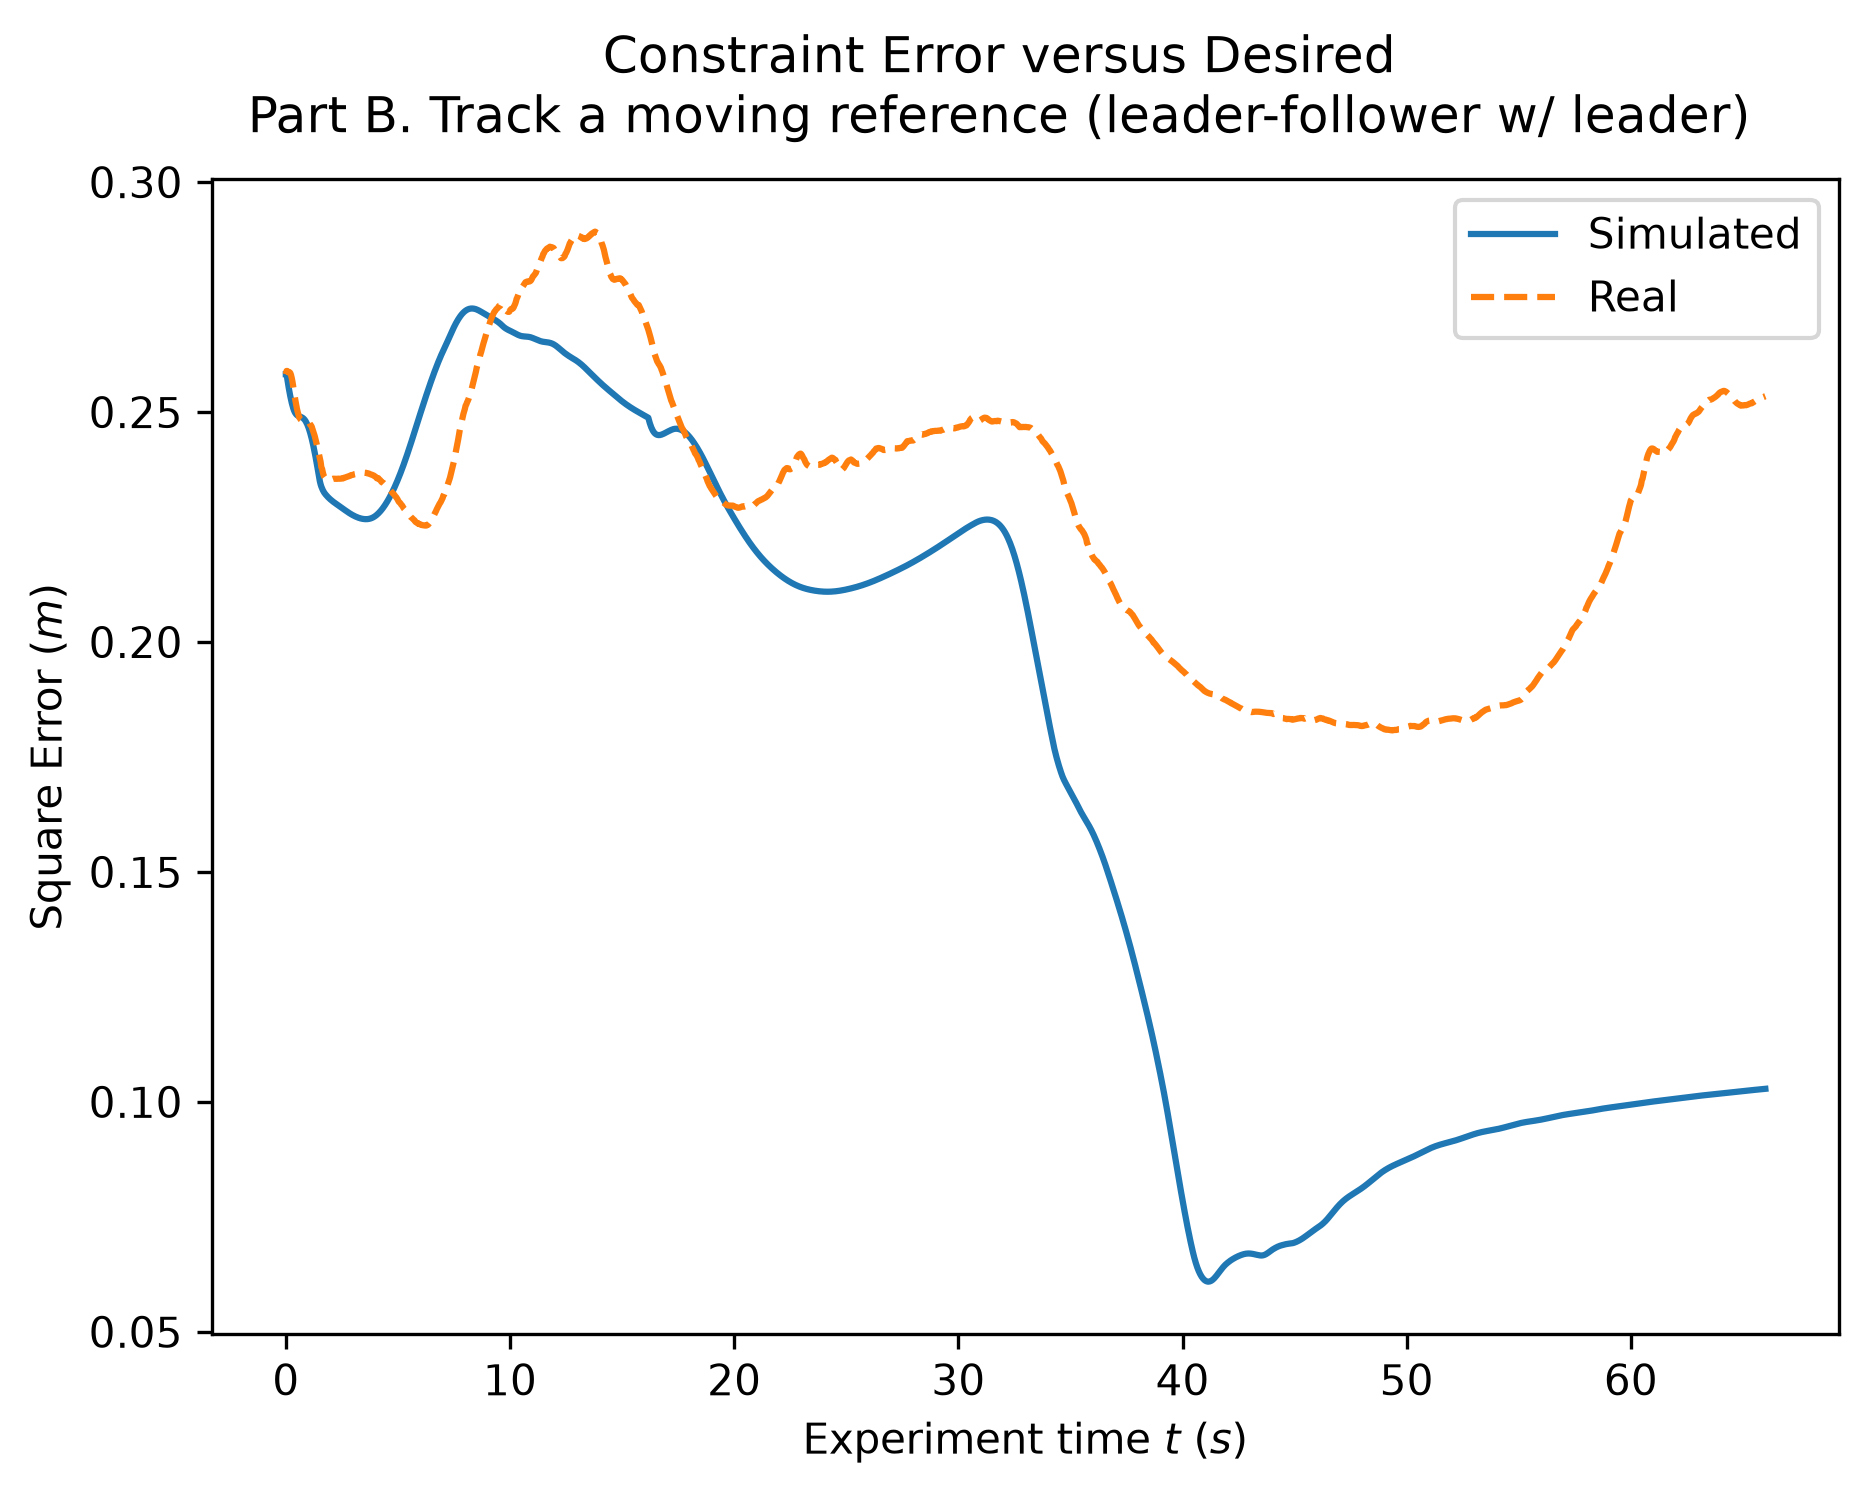
\includegraphics[width=\textwidth]{Figures/b_leader_const_error.png}
        \captionsetup{justification=centering}
        \caption{Distance constraint error for total formation for leader-follower moving reference formation control.}
        % \label{fig:}
    \end{subfigure}\hfill
    \begin{subfigure}[t]{0.45\textwidth}
        \centering
        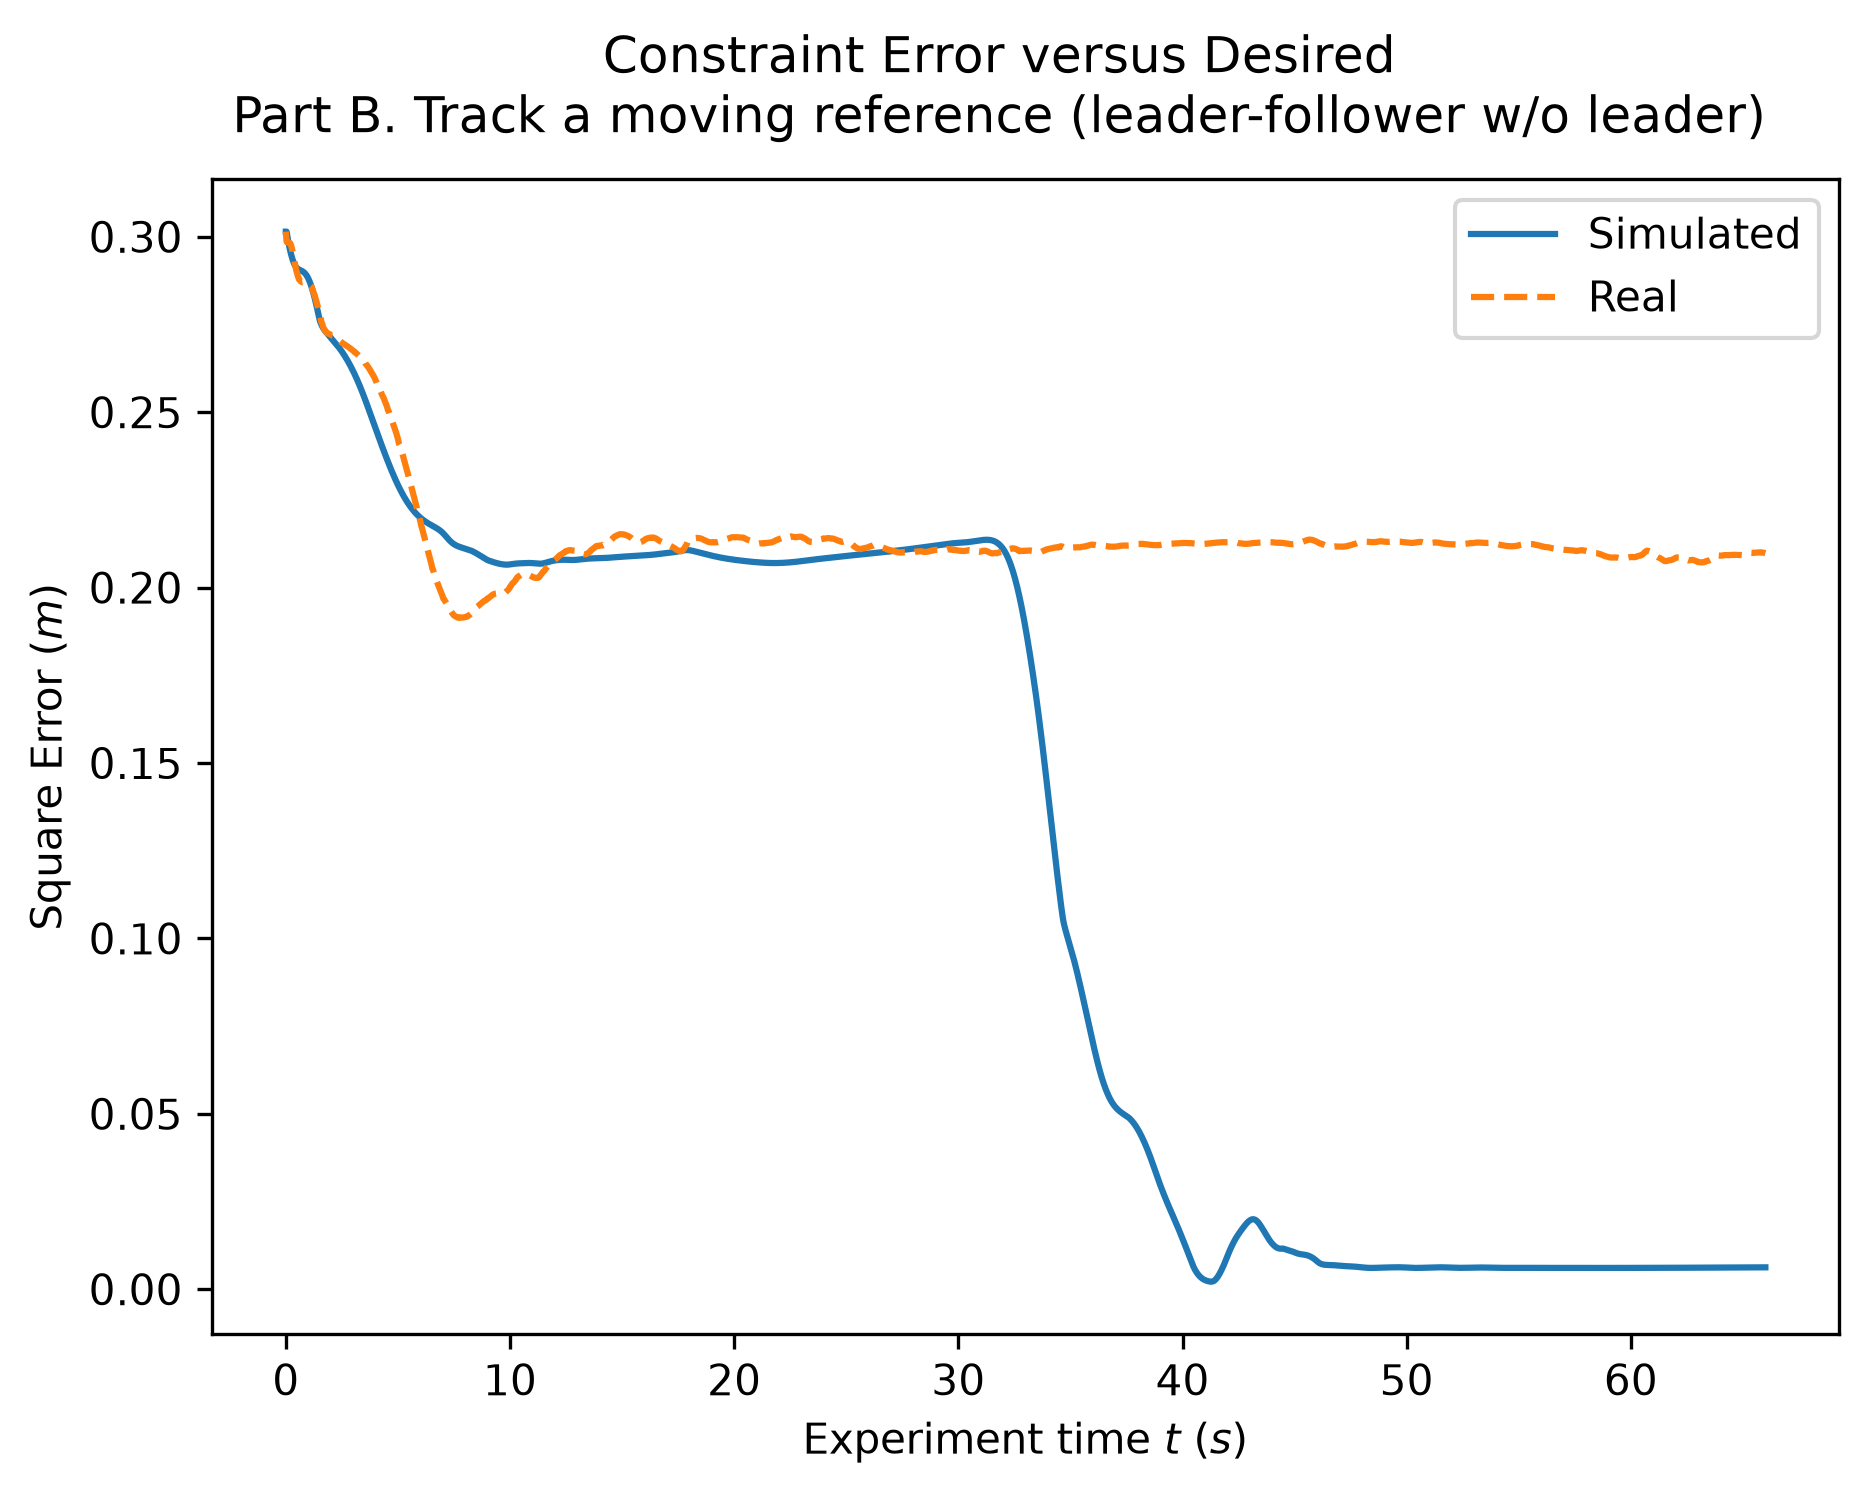
\includegraphics[width=\textwidth]{Figures/b_leader_fol_const_error.png}
        \captionsetup{justification=centering}
        \caption{Distance constraint error for follower formation for leader-follower moving reference formation control.}
        % \label{fig:}
    \end{subfigure}
    \captionsetup{justification=centering}
    \caption{Distance constraint error for simulation and hardware robot leader-follower moving reference formation control.}
    \label{fig:dist_b_l}
\end{figure}

\clearpage
\subsection*{C. Proximity-based communication}
Write a helper function that takes the current robot positions and a communication radius $R>0$ and returns the adjacency matrix
\begin{align*}
    A_{ij}(t)&=\begin{cases}
        1, & i\neq j\ \text{and}\ \|p_j(t)-p_i(t)\|<R\,,\\
        0, & \text{otherwise}\,.
    \end{cases}
\end{align*}
Rerun the distance-based controller from part A in simulation and hardware, updating the communication graph at every step of the simulation loop according to the above proximity-based construction. Choose and report $R$, and use $d_{ij}=\|q_j-q_i\|$ for every pair that communicates, where $q_i$ are you desired formation coordinates. Use the same initial conditions and include the same plots as in part A. For comparison, evaluate $E_d(t)$ using the original fixed edge set from Part A. How does proximity-based communication affect convergence and the final formation?

\subsubsection*{ANSWER:}
For the proximity-based communication, the formation and graph from Part A was utilized ((\ref{eqn:p_ac}) and (\ref{eqn:graph_ac}), with the exception that the adjacency matrix in (\ref{eqn:al_ac}) were set to zero if the robots were not in proximity $R$ of each other. For these experiments, $R=1\ m$. Because of this, \textit{all} of the distance constraints in (\ref{eqn:graph_ac}) were able to be met through direct robot communication \textit{except} for the redundant edge between robot 2 and robot 6 of distance $1.6\ m$. The resulting robot trajectories are given in Figure \ref{fig:traj_c}. As seen, when comparing to the trajectories from Figure \ref{fig:traj_a}, even from the same initial conditions, the results are \textit{not} the same. The desired formation in Figure \ref{fig:formation} was not achieved in either proximity-based experiment, and the reason was, even though the graph without the redundant edge between robots 2 and 6 was still found to be rigid, it is not \textit{persistent}, as there are multiple configurations that can achieve all of the distance constraints while failing the formation, such as ``folding'' the triangle in half such that the two lower corners are on top of each other. This was the formation that the robots were trying to settle to in these proximity-based experiments, where vertically mirrored robots would share final coordinates, but, because of the safety collision controller, they could not do so, and so the formation simply fails. Even when robots 2 and 6 (green and brown in the Figure) get into range of each other to properly communicate, if they are already both ``trapped'' behind the ``wall'' of other robots, they will not be able to move to the opposite side. Given different initial conditions, however, with robots 2 and 6 already on opposite sides of the area, it is likely the formation would be achieved for this given $R$.

\begin{figure}[htb]
    \centering
    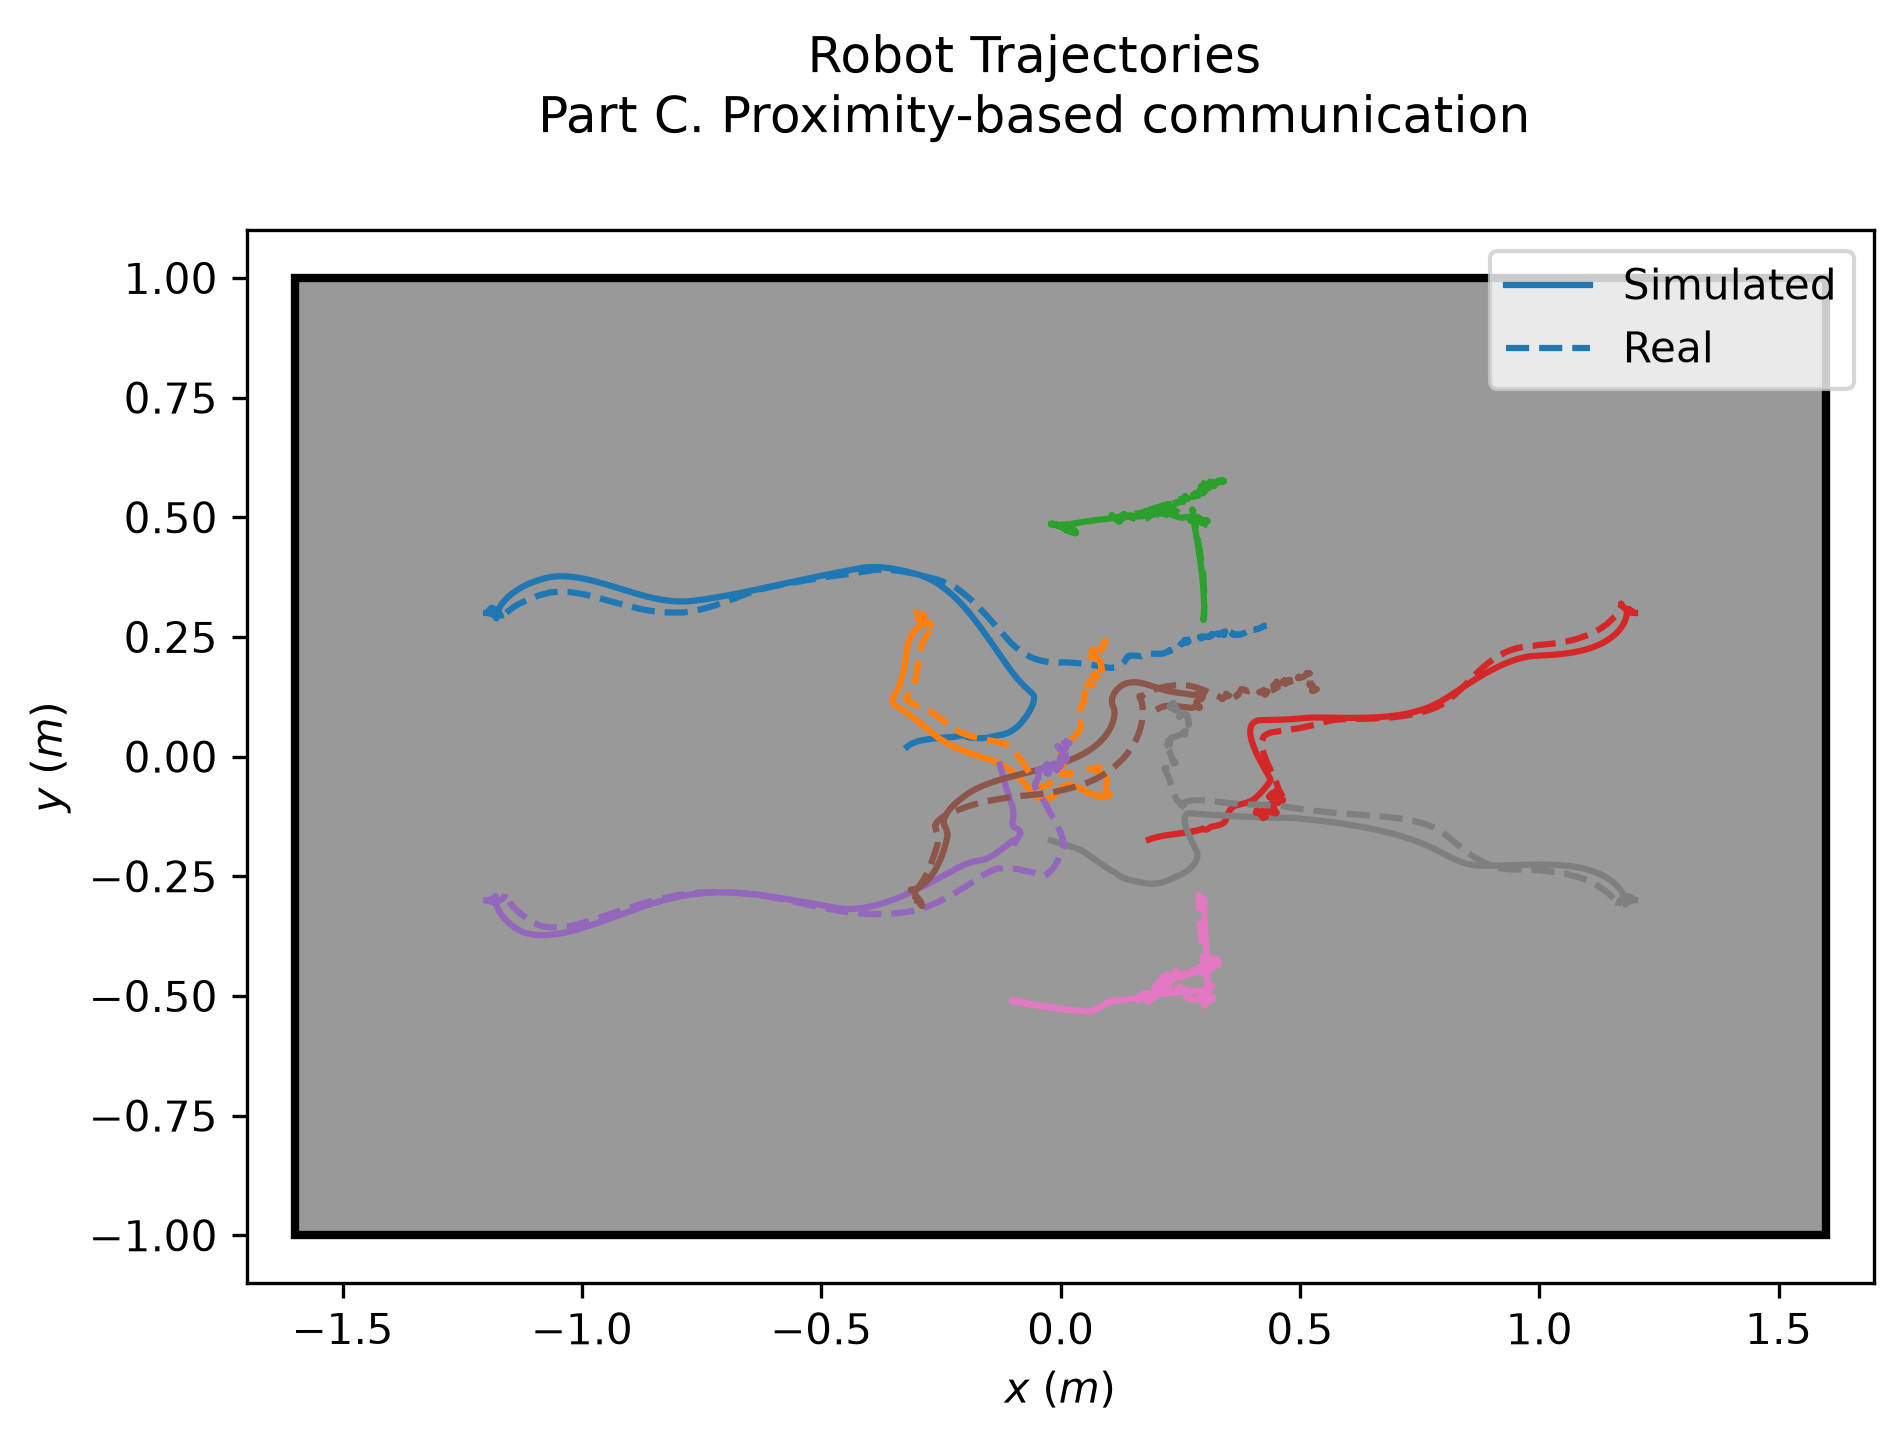
\includegraphics[width=0.5\textwidth]{Figures/c_traj_dist.png}
    \captionsetup{justification=centering}
    \caption{Simulation and hardware robot trajectories for proximity-based communication formation control.}
    \label{fig:traj_c}
\end{figure}

\FloatBarrier
Figure \ref{fig:dist_square_c} provides the distance constraint error between the formation in (\ref{eqn:graph_ac}) and the simulation/hardware results, as well as the square error between the simulation and hardware results. As seen, while the formation \textit{does} converge towards the desired distances, it ``bottoms out'' because of the safety barrier functions preventing overlapping coordinates, as well as the fact that robots 2 and 6 (green and brown in Figure \ref{fig:traj_c}) are stuck too near each other and unable to separate. The square error between the simulation and the hardware experiments, as expected, grows over time, although nowhere as drastically as in Figure \ref{fig:square_way_b}, where the results diverged, but certainly more than in the original distance-based and displacement-based experiments in Figure \ref{fig:square_a}. The hypothesized reason for this is that once the robots begin interacting with the control barrier functions (as in, when they get too close), their behavior is much more difficult to simulate, and small deviations can cause large drifts, which was what is seen in Figure \ref{fig:traj_c}, for example, with robot 4 (the gray trajectory). Therefore, proximity-based communication adds additional complexity to formation control and its ability to converge to the desired formation. Either the robots need to have greater communication radii $R$, or there need to be more distance constraints and redundant edges to account for the loss of rigidity through communication regions, increasing the complexity of the formation design.

\begin{figure}[htb]
    \centering
    \begin{subfigure}[t]{0.45\textwidth}
        \centering
        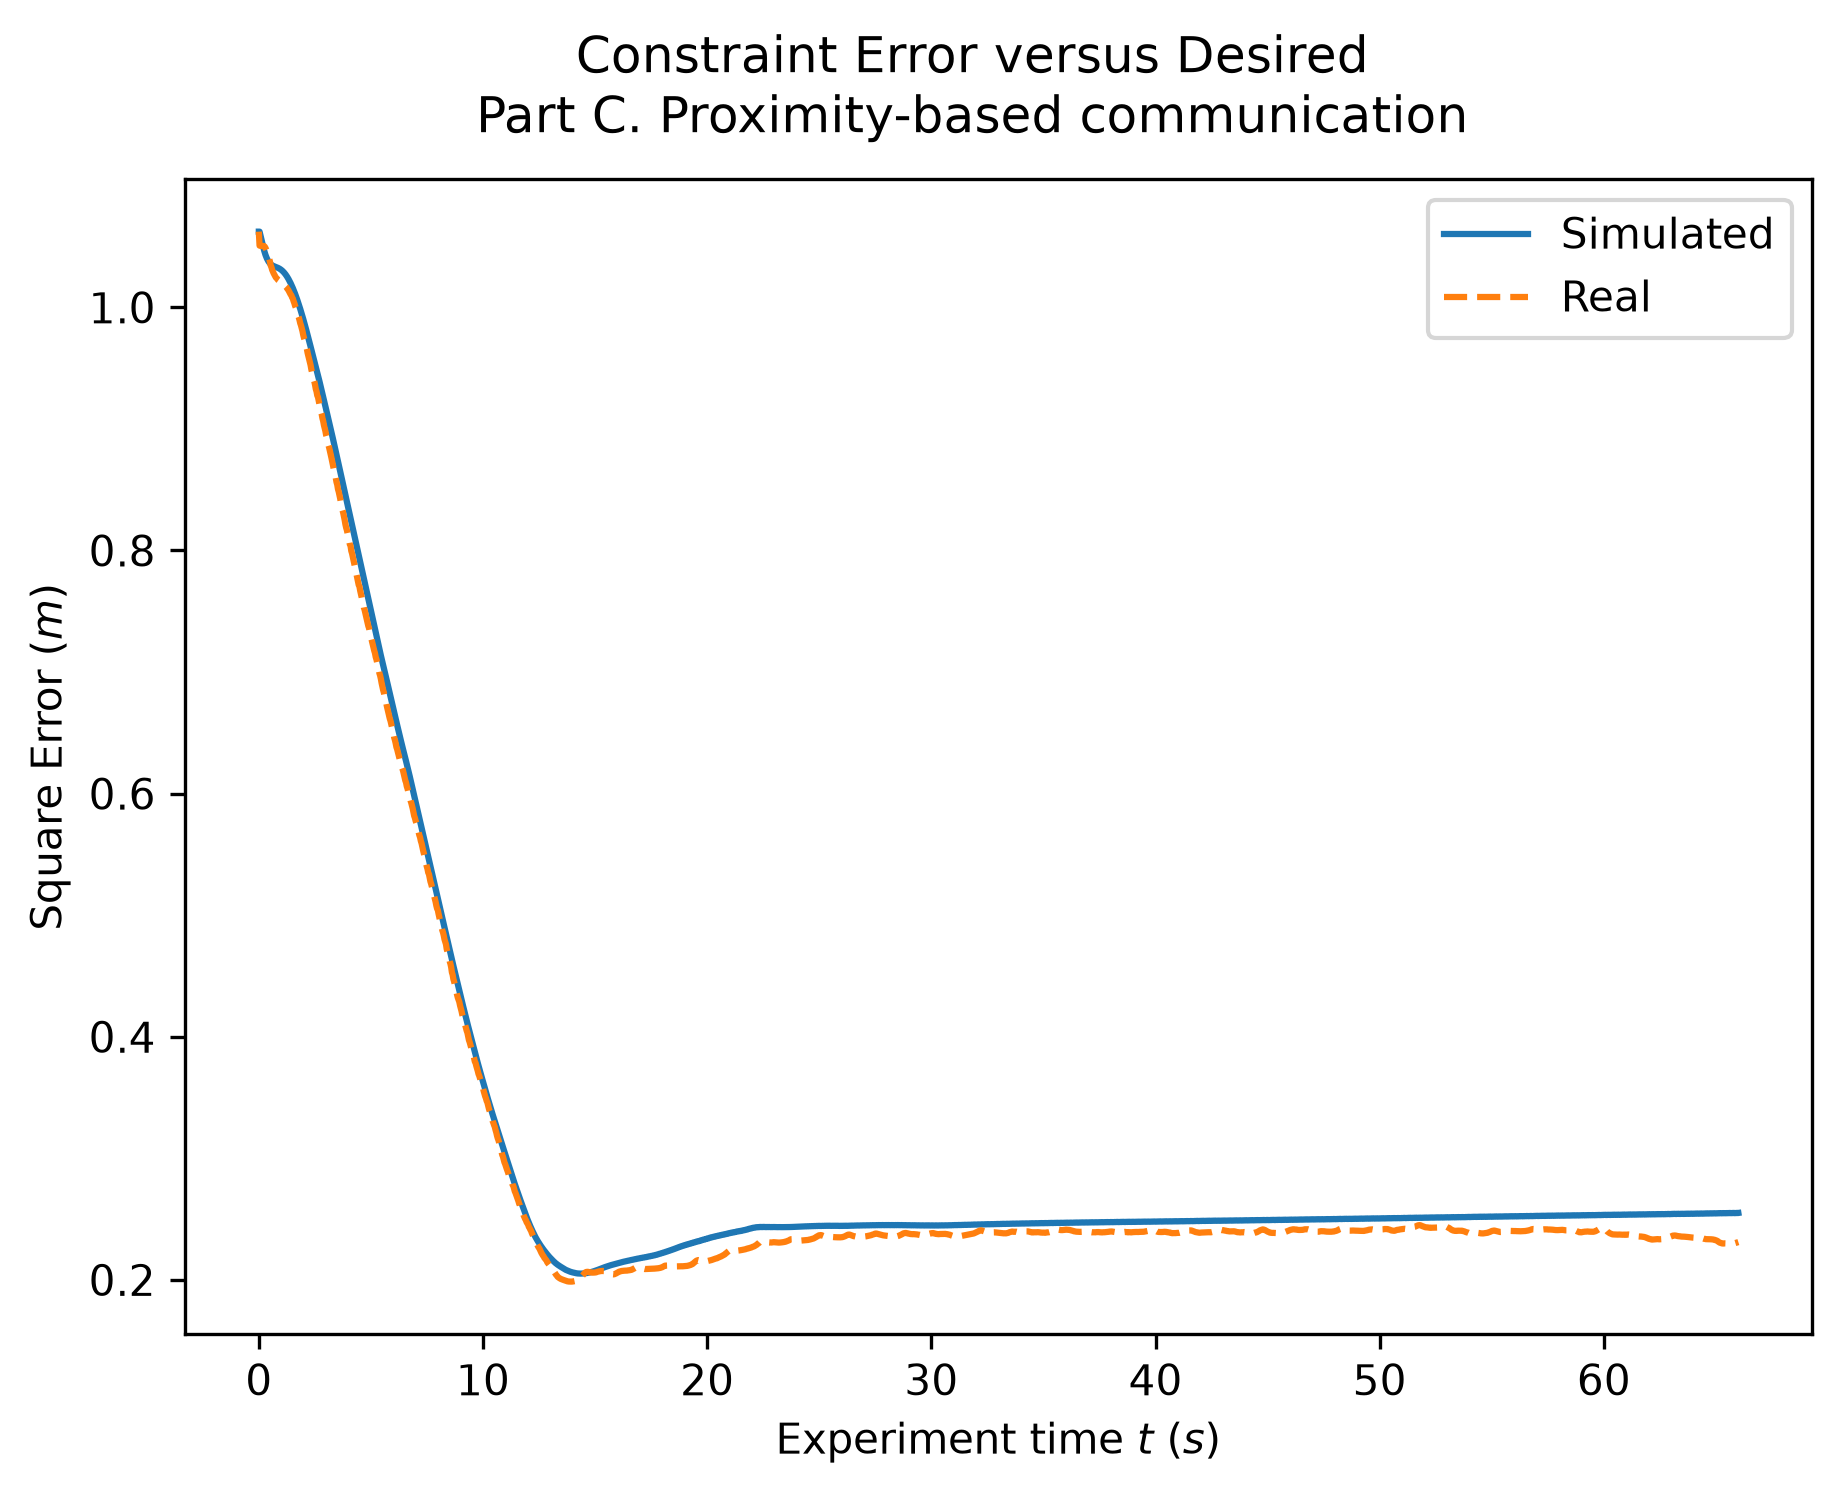
\includegraphics[width=\textwidth]{Figures/c_const_error.png}
        \captionsetup{justification=centering}
        \caption{Simulation and hardware distance constraint error for proximity-based communication formation control.}
        % \label{fig:}
    \end{subfigure}\hfill
    \begin{subfigure}[t]{0.45\textwidth}
        \centering
        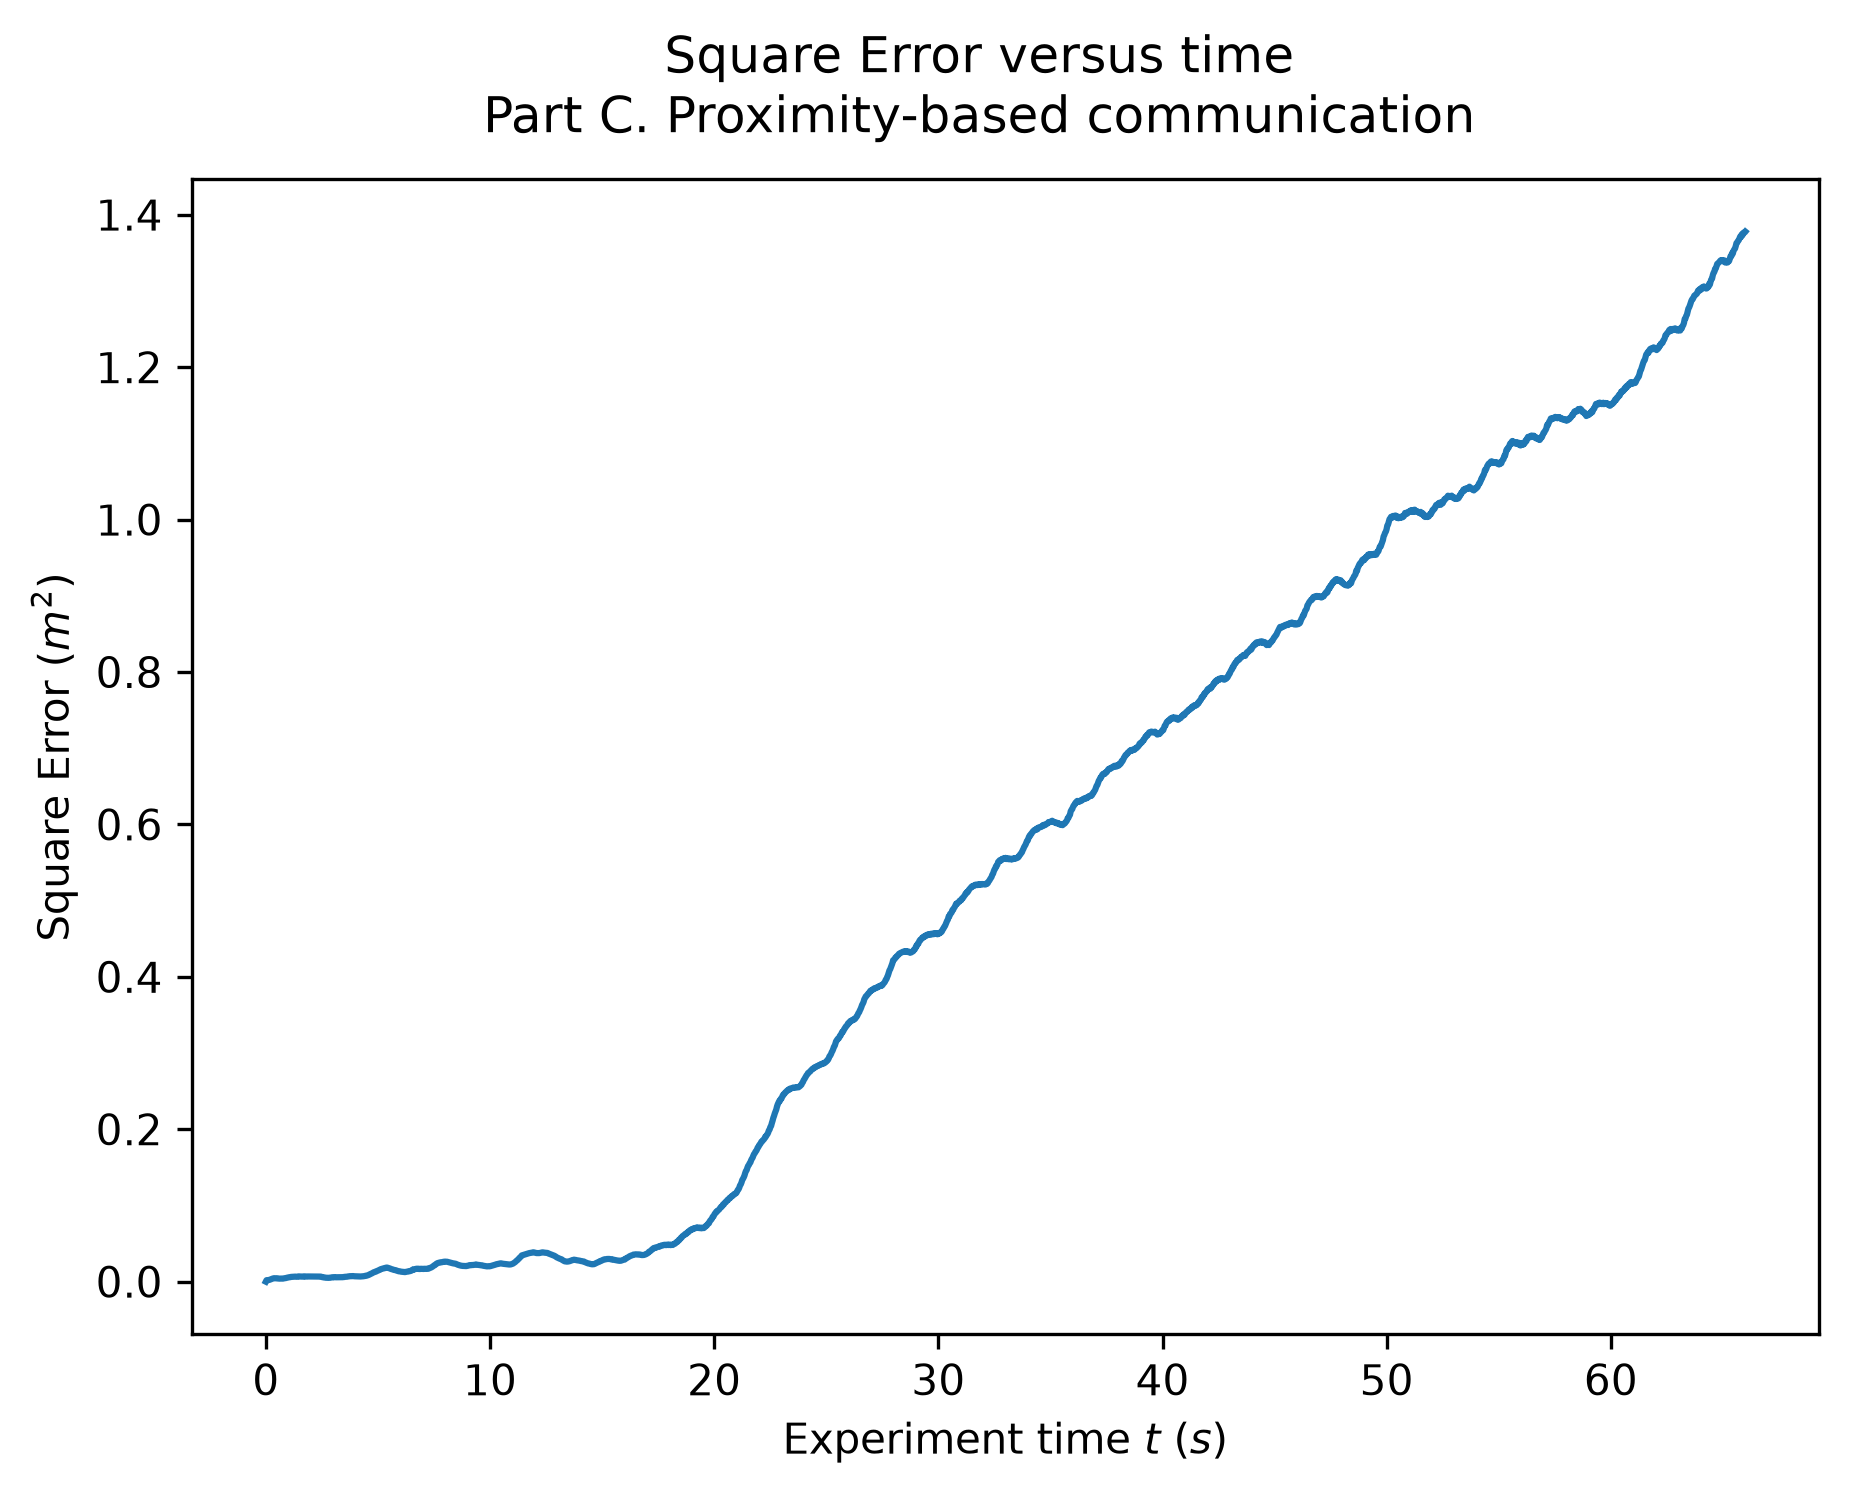
\includegraphics[width=\textwidth]{Figures/c_square_error.png}
        \captionsetup{justification=centering}
        \caption{Square error between $p^{real}(t)$ and $p^{sim}(t)$ for proximity-based communication formation control.}
        % \label{fig:}
    \end{subfigure}
    \captionsetup{justification=centering}
    \caption{Errors for proximity-based formation control.}
    \label{fig:dist_square_c}
\end{figure}

\clearpage
\section*{PROBLEM SOLUTIONS (Part 2: Flocking) (BASED ON JULIAN'S WORK)}
Next, we will use the following implementation of Reynolds' Boids model to control the motion of our robots:
\begin{align*}
    \dot p_i&=v_i & \dot v_i&=u_i & \mathcal N_i(t)&=\{j\neq i:\|p_i(t)-p_i(t)\|<R\}
\end{align*}
\begin{align*}
    u_i&=k_s\sum_{j\in\mathcal N_i}\frac{p_i-p_j}{\|p_i-p_j\|^2+\epsilon^2}+\frac{k_a}{|\mathcal N_i|}\sum_{j\in\mathcal N_i}(v_j-v_i)+\frac{k_c}{|\mathcal N_i|}\sum_{j\in\mathcal N_i}(p_j-p_i)+b_i[k_p(w_\ell-p_i)-k_vv_i]\,.
\end{align*}
The first three terms represent separation, alignment, and cohesion with gains $k_s,k_a,k_c>0$ that you define and the fourth term represents steering towards waypoint $w_\ell$ (choice of waypoint may switch during operation); try the following parameters as a starting point (that you may modify to suit your own experiment as needed):
\begin{align*}
    \epsilon&=0.01 & k_s&=0.01 & k_a&=1 & k_c&=0.25 & k_p&=0.2 & k_v=1 & R&=0.75\,.
\end{align*}
You may choose any number of robots between 5 and 16 for your flock size.

\subsection*{1.}
Implement the flocking controller, reusing your helper function from Part 1C to construct the proximity graph. Since the Robotarium accepts velocity commands, you will first need to derive a discrete-time velocity update from the acceleration $u_i$. State how you initialize the velocities and obtain the velocity values used in the controller.

\subsection*{ANSWER:}
To derive a discrete-time velocity update from the acceleration command $u_i$, we can apply a single-step Euler discretization such that
\begin{align*}
    v_i[k]&=v_i[k-1]+\Delta tu_i[k]\,,
\end{align*}
where $\Delta t$ is the time step within the simulator ($\Delta t=0.033\ s$). From there, the new velocities $v_i[k]$ are passed into the saturation function to ensure that the desired magnitude of the command is achievable by the robot as
\begin{align*}
    \hat v_i[k]&=v_i[k]*\min\left\{1,\frac{v_{max}}{\|v_i[k]\|}\right\}\,,
\end{align*}
which is then passed into the \texttt{si\_barrier\_cert} and \texttt{si\_to\_uni\_dynamics} to ensure that there are no collisions and to convert the idealized single-integrator velocity approximation into unicycle robot commands for the robot's morphology. For these experiments, all robots were initialized with $v_i[0]=0$.

For the following flocking experiments, $N=6$ robots were used, and the waypoints were given coordinates of (in meters $m$)
\begin{align*}
    w_1&=(-1,0.75) & w_2&=(-1,-0.75) & w_3&=(1,-0.75) & w_4&=(1,0.75)\,,
\end{align*}
and the tolerance for waypoint switching (either by average flock position/centroid or leader position) was set at $\epsilon=0.15\ m$.

Metrics for velocity alignment and flocking performance that were used to analyze the results are
\begin{enumerate}
    \item Polarization $\psi(t)=\|\sum_iv_i\|/\sum_i\|v_i\|\in[0,1]$, which is equal to 1 when all robots move in exactly the same direction for any speeds and 0 when they move in totally opposite directions.
    \item Velocity variance $\sigma_v^2(t)=\frac 1N\sum_i\|v_i-\bar v\|^2$, where $\bar v$ is the average velocity of the flock.
    \item Cohesion: number of connected components of the proximity-based communication graph and the maximum pairwise distance between any two robots in the flock.
    \item Waypoint following: distance from the monitored point (either the average flock position/centroid or the leader's position) from the active waypoint coordinates.
    \item Square error $E_{sim}(t)=\sum_{i\in\mathcal V}\|p_i^{real}(t)-p_i^{sim}(t)\|^2$.
\end{enumerate}

\clearpage
\subsection*{2.}
Set $b_i=1$ for every robot and move the flock through the same waypoint sequence as in Part 1B (this means all robots have access to the motion plan). You will need to decide on a rile to advance the waypoint selection from one to the next, e.g., based on proximity of the centroid of the froup or of the closest number. Run the controller in simulation and hardware from shared initial conditions. Plot the robot trajectories, measures of velocity alignment that you define, and $E_{sim}(t)$. In your report, discuss how the resulting motion compares with your formation control experiments, and any discrepancies between simulation and experiment.

\subsection*{ANSWER:}
The flocking algorithm was run with the default parameters with waypoint switching governed by proximity of the \textit{average flock position/centroid}. Figure \ref{fig:traj_2} shows the trajectories for both the simulated and hardware experiments. As seen, the simulation matches closely with the hardware, with slight discrepancies causes by imperfect simulation conditions explored during the formation-control experiments that cause the square error to grow over time (Figure \ref{fig:square_2}). Initially, as seen by the trajectories, all of the robots began separated from one another, so the communication graph was empty. This would not work in a leader-follower configuration, especially since initial velocities $v_i[0]=0$, but since all robots knew the waypoint plan, they individually moved towards the target. Once they were within the sensing radius $R$, the flock was formed and seemed to maintain cohesion throughout the rest of the trajectory.

\begin{figure}[htb]
    \centering
    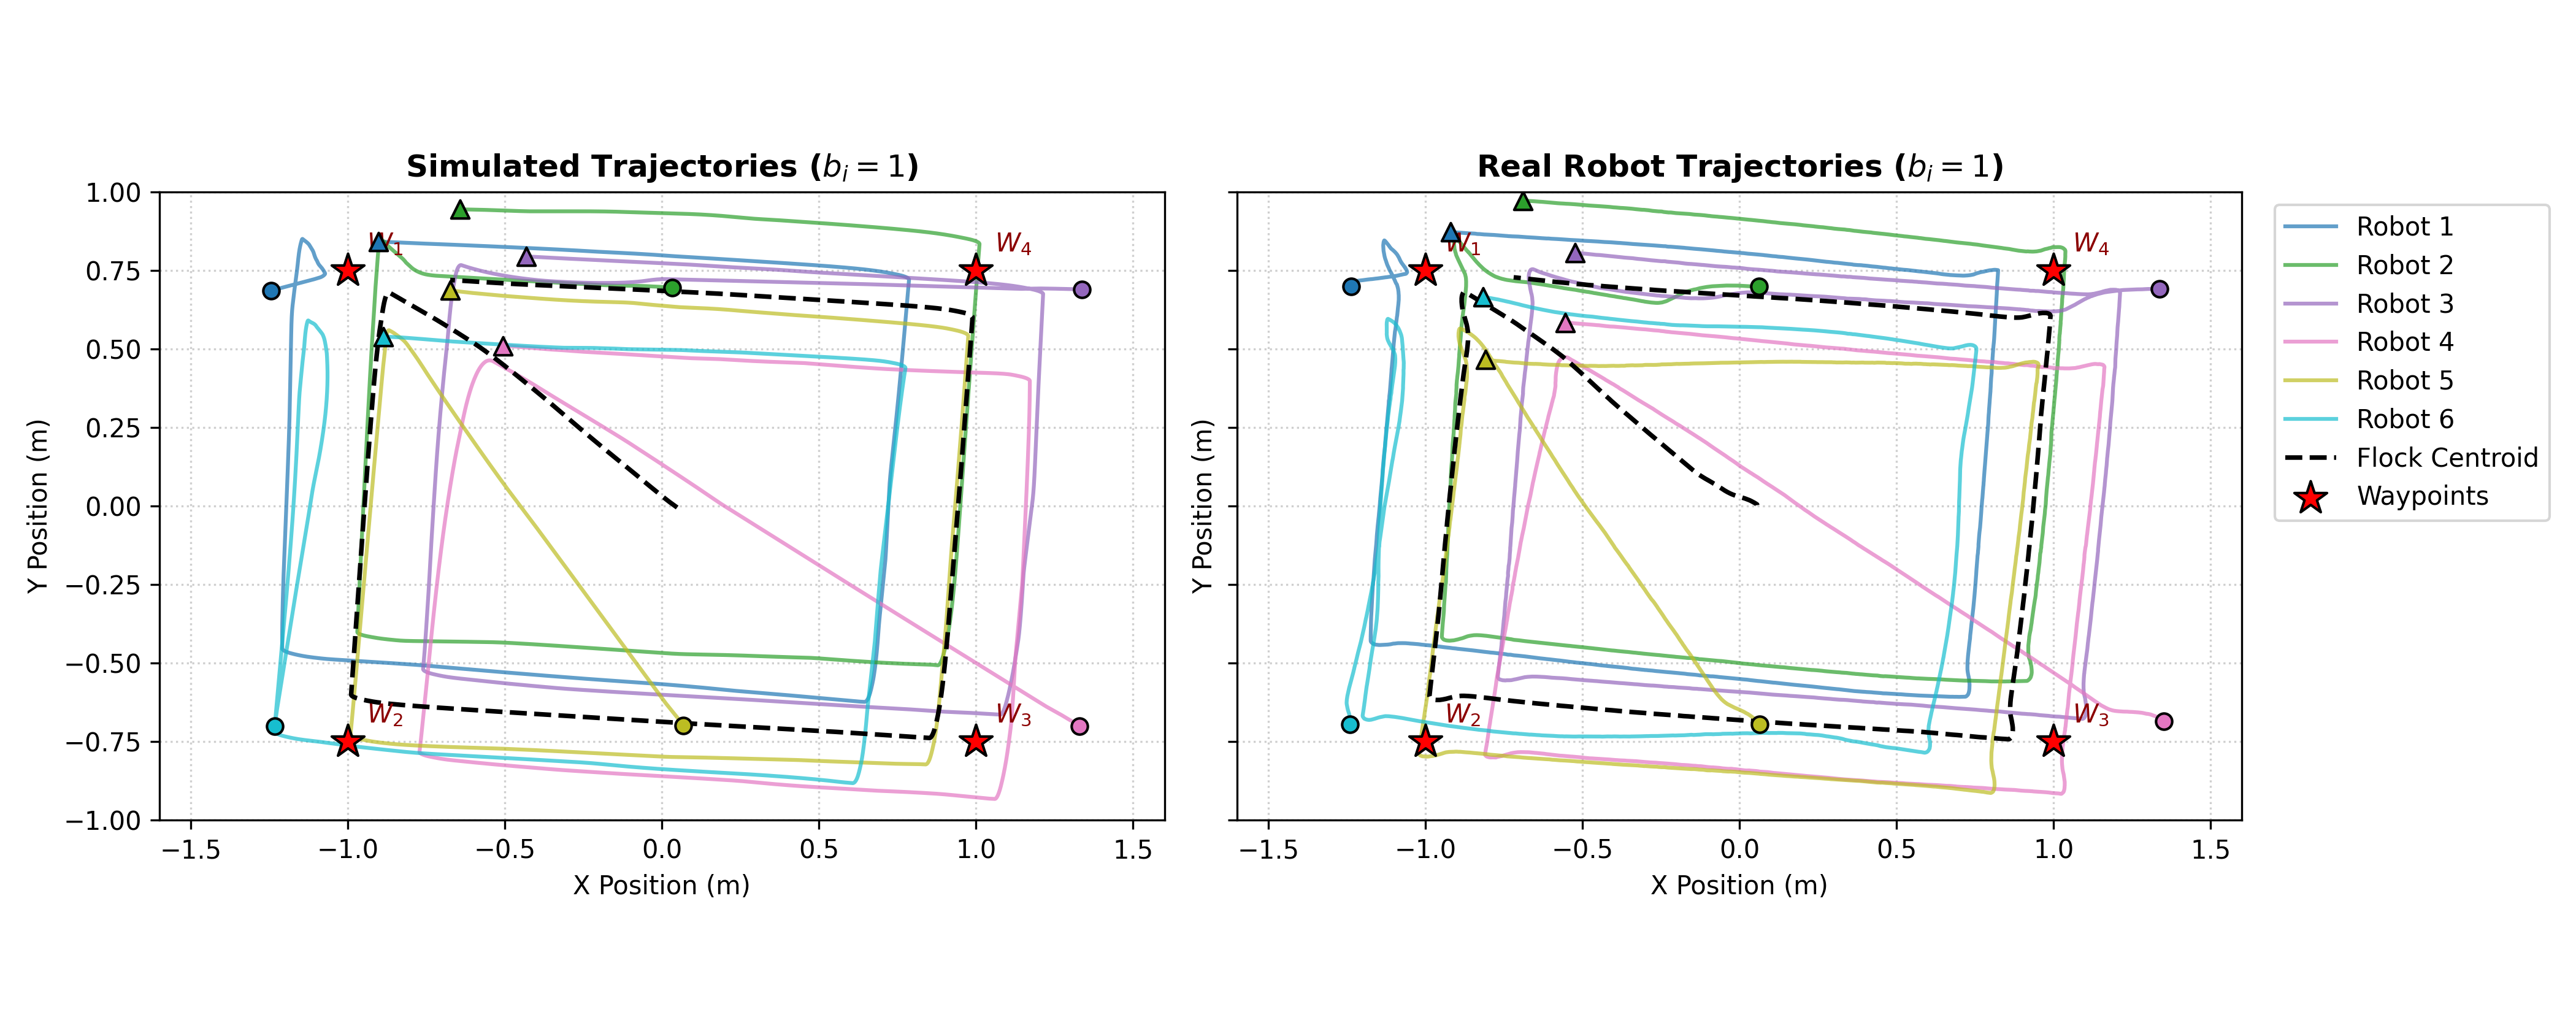
\includegraphics[width=0.9\textwidth]{Figures/part2_sec2_trajectories.png}
    \captionsetup{justification=centering}
    \caption{Simulation and hardware robot trajectories for global-knowledge flocking control.}
    \label{fig:traj_2}
\end{figure}

\begin{figure}[htb]
    \centering
    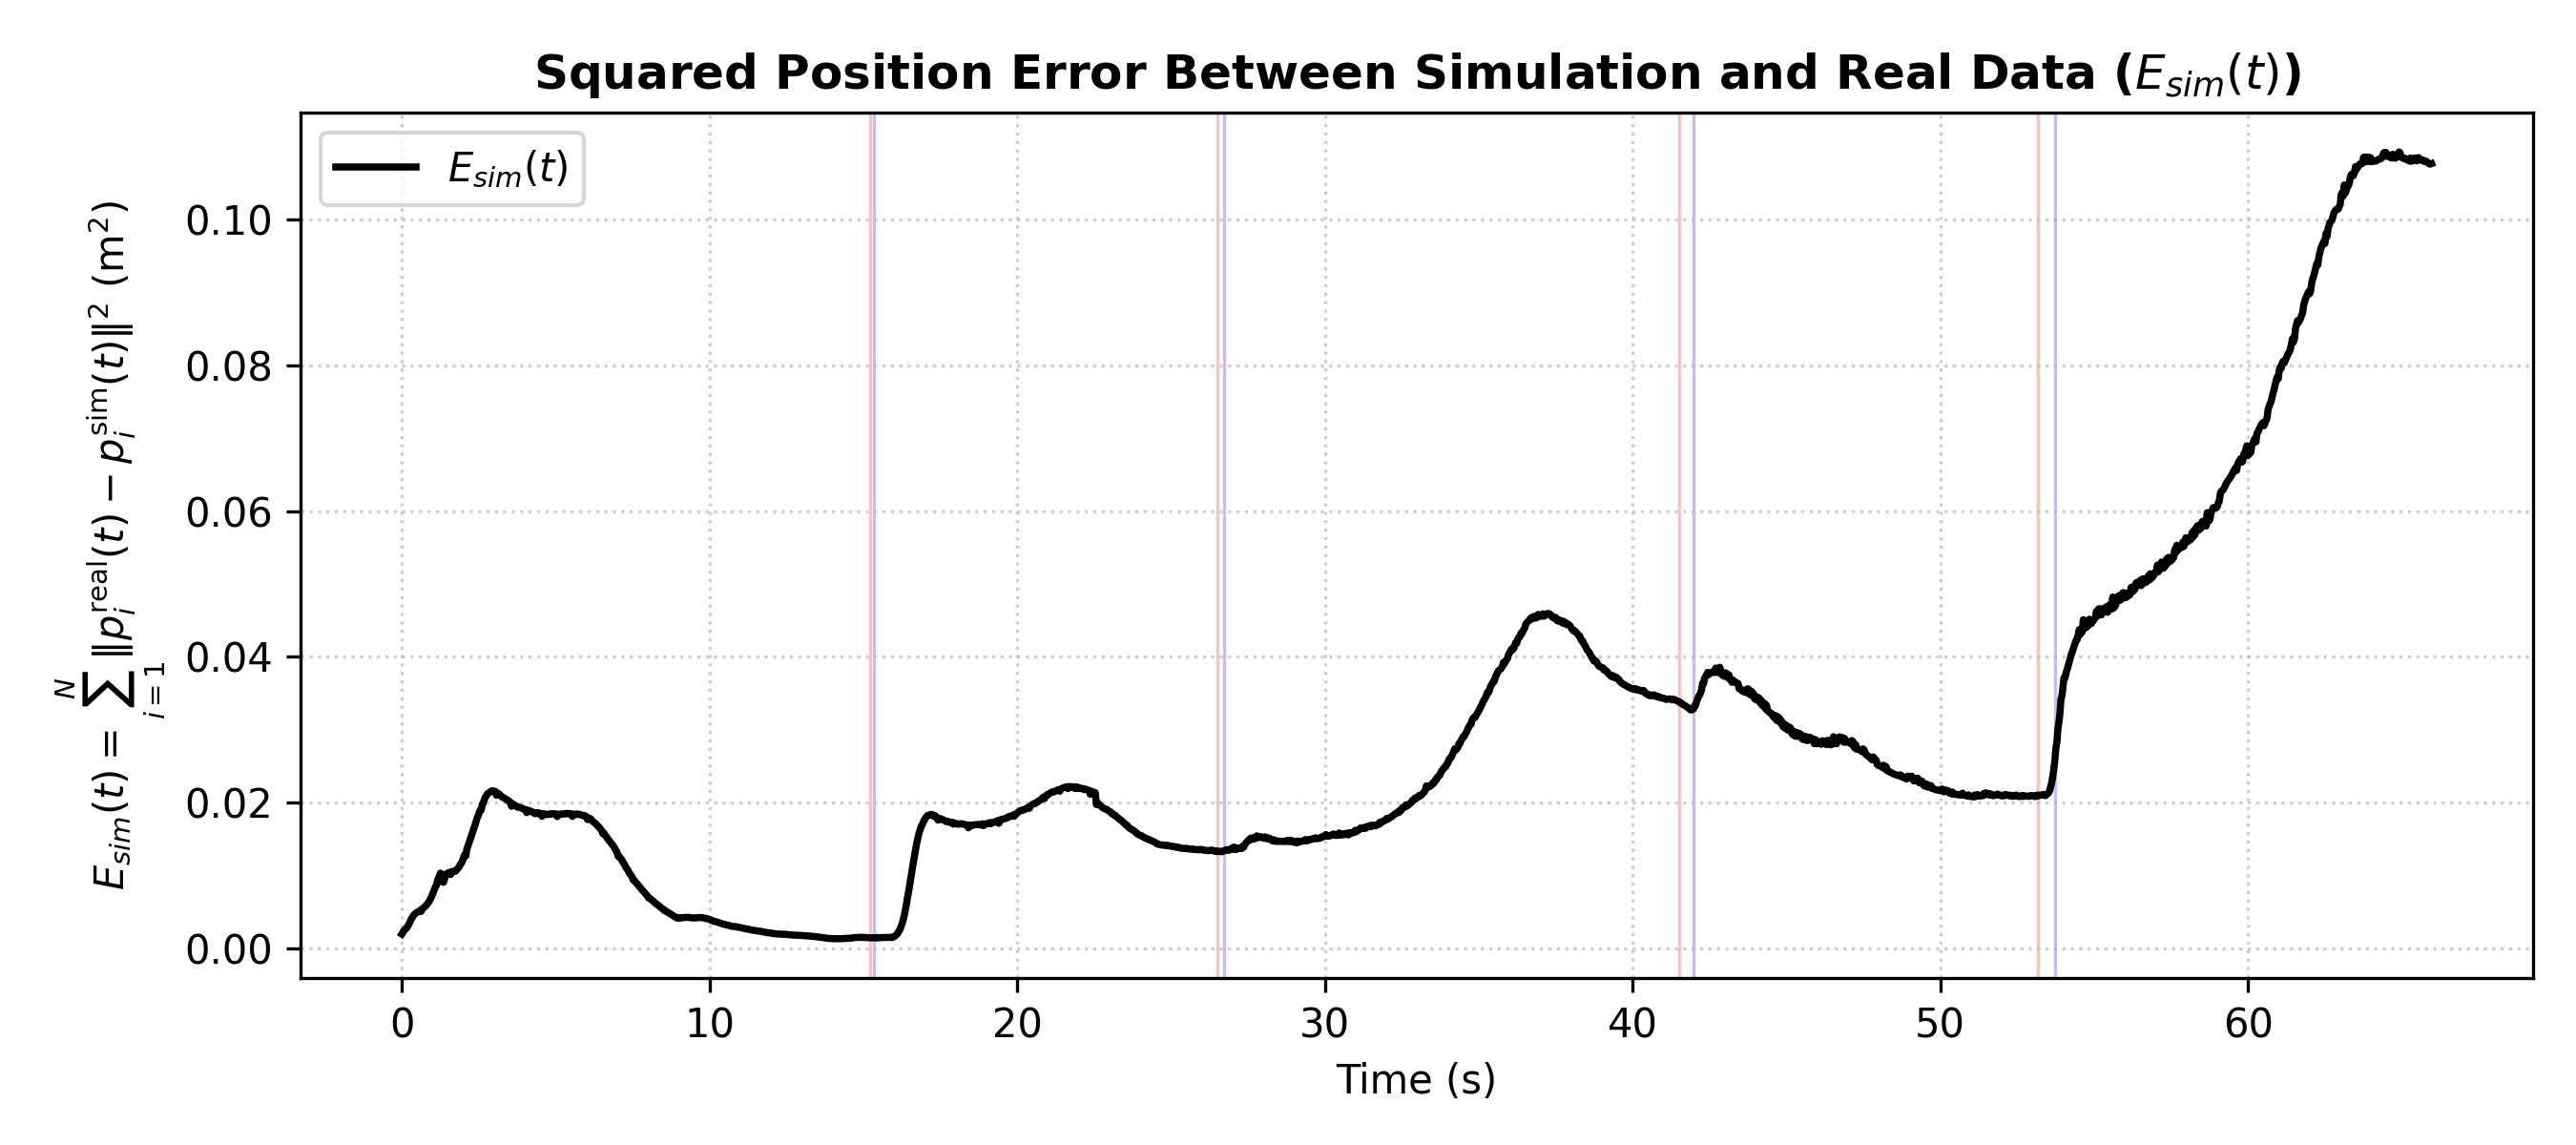
\includegraphics[width=0.8\textwidth]{Figures/part2_sec2_E_sim.png}
    \captionsetup{justification=centering}
    \caption{Square error between $p^{real}(t)$ and $p^{sim}(t)$ for global-knowledge flocking control.}
    \label{fig:square_2}
\end{figure}

\FloatBarrier
To better understand the flocking performance, the velocity alignment metrics $\psi(t)$ and $\sigma_v^2(t)$ are plotted in Figure \ref{fig:metrics_2}, along with the number of robots moving for any given $t$. As seen, and as expected, since all robots initially began moving individually to the waypoint from their initial positions, the variance is high and the polarization is low. However, at about $\sim17\ s$, when the flock is formed, the variance decreases to zero as they all match their speeds and the polarization increases to 1, showing that the flock maintained its shape and heading. There are slight ``blips'' when the variance increases and the number of moving robots decreases from 6 to 5, but this is caused by the control barrier functions preventing robots from colliding during flock maneuvers. Overall, with global-knowledge of the waypoint plan, the flock was able to stay together, which shouldn't be surprising as all robots move towards a shared goal, whether they are flocked or not. This is similar to the formation results in Figures \ref{fig:traj_dist_global_b}, where the shape was maintained throughout the experiments simply because each robot moved individually on its own relative to the shared reference point.

\begin{figure}[htb]
    \centering
    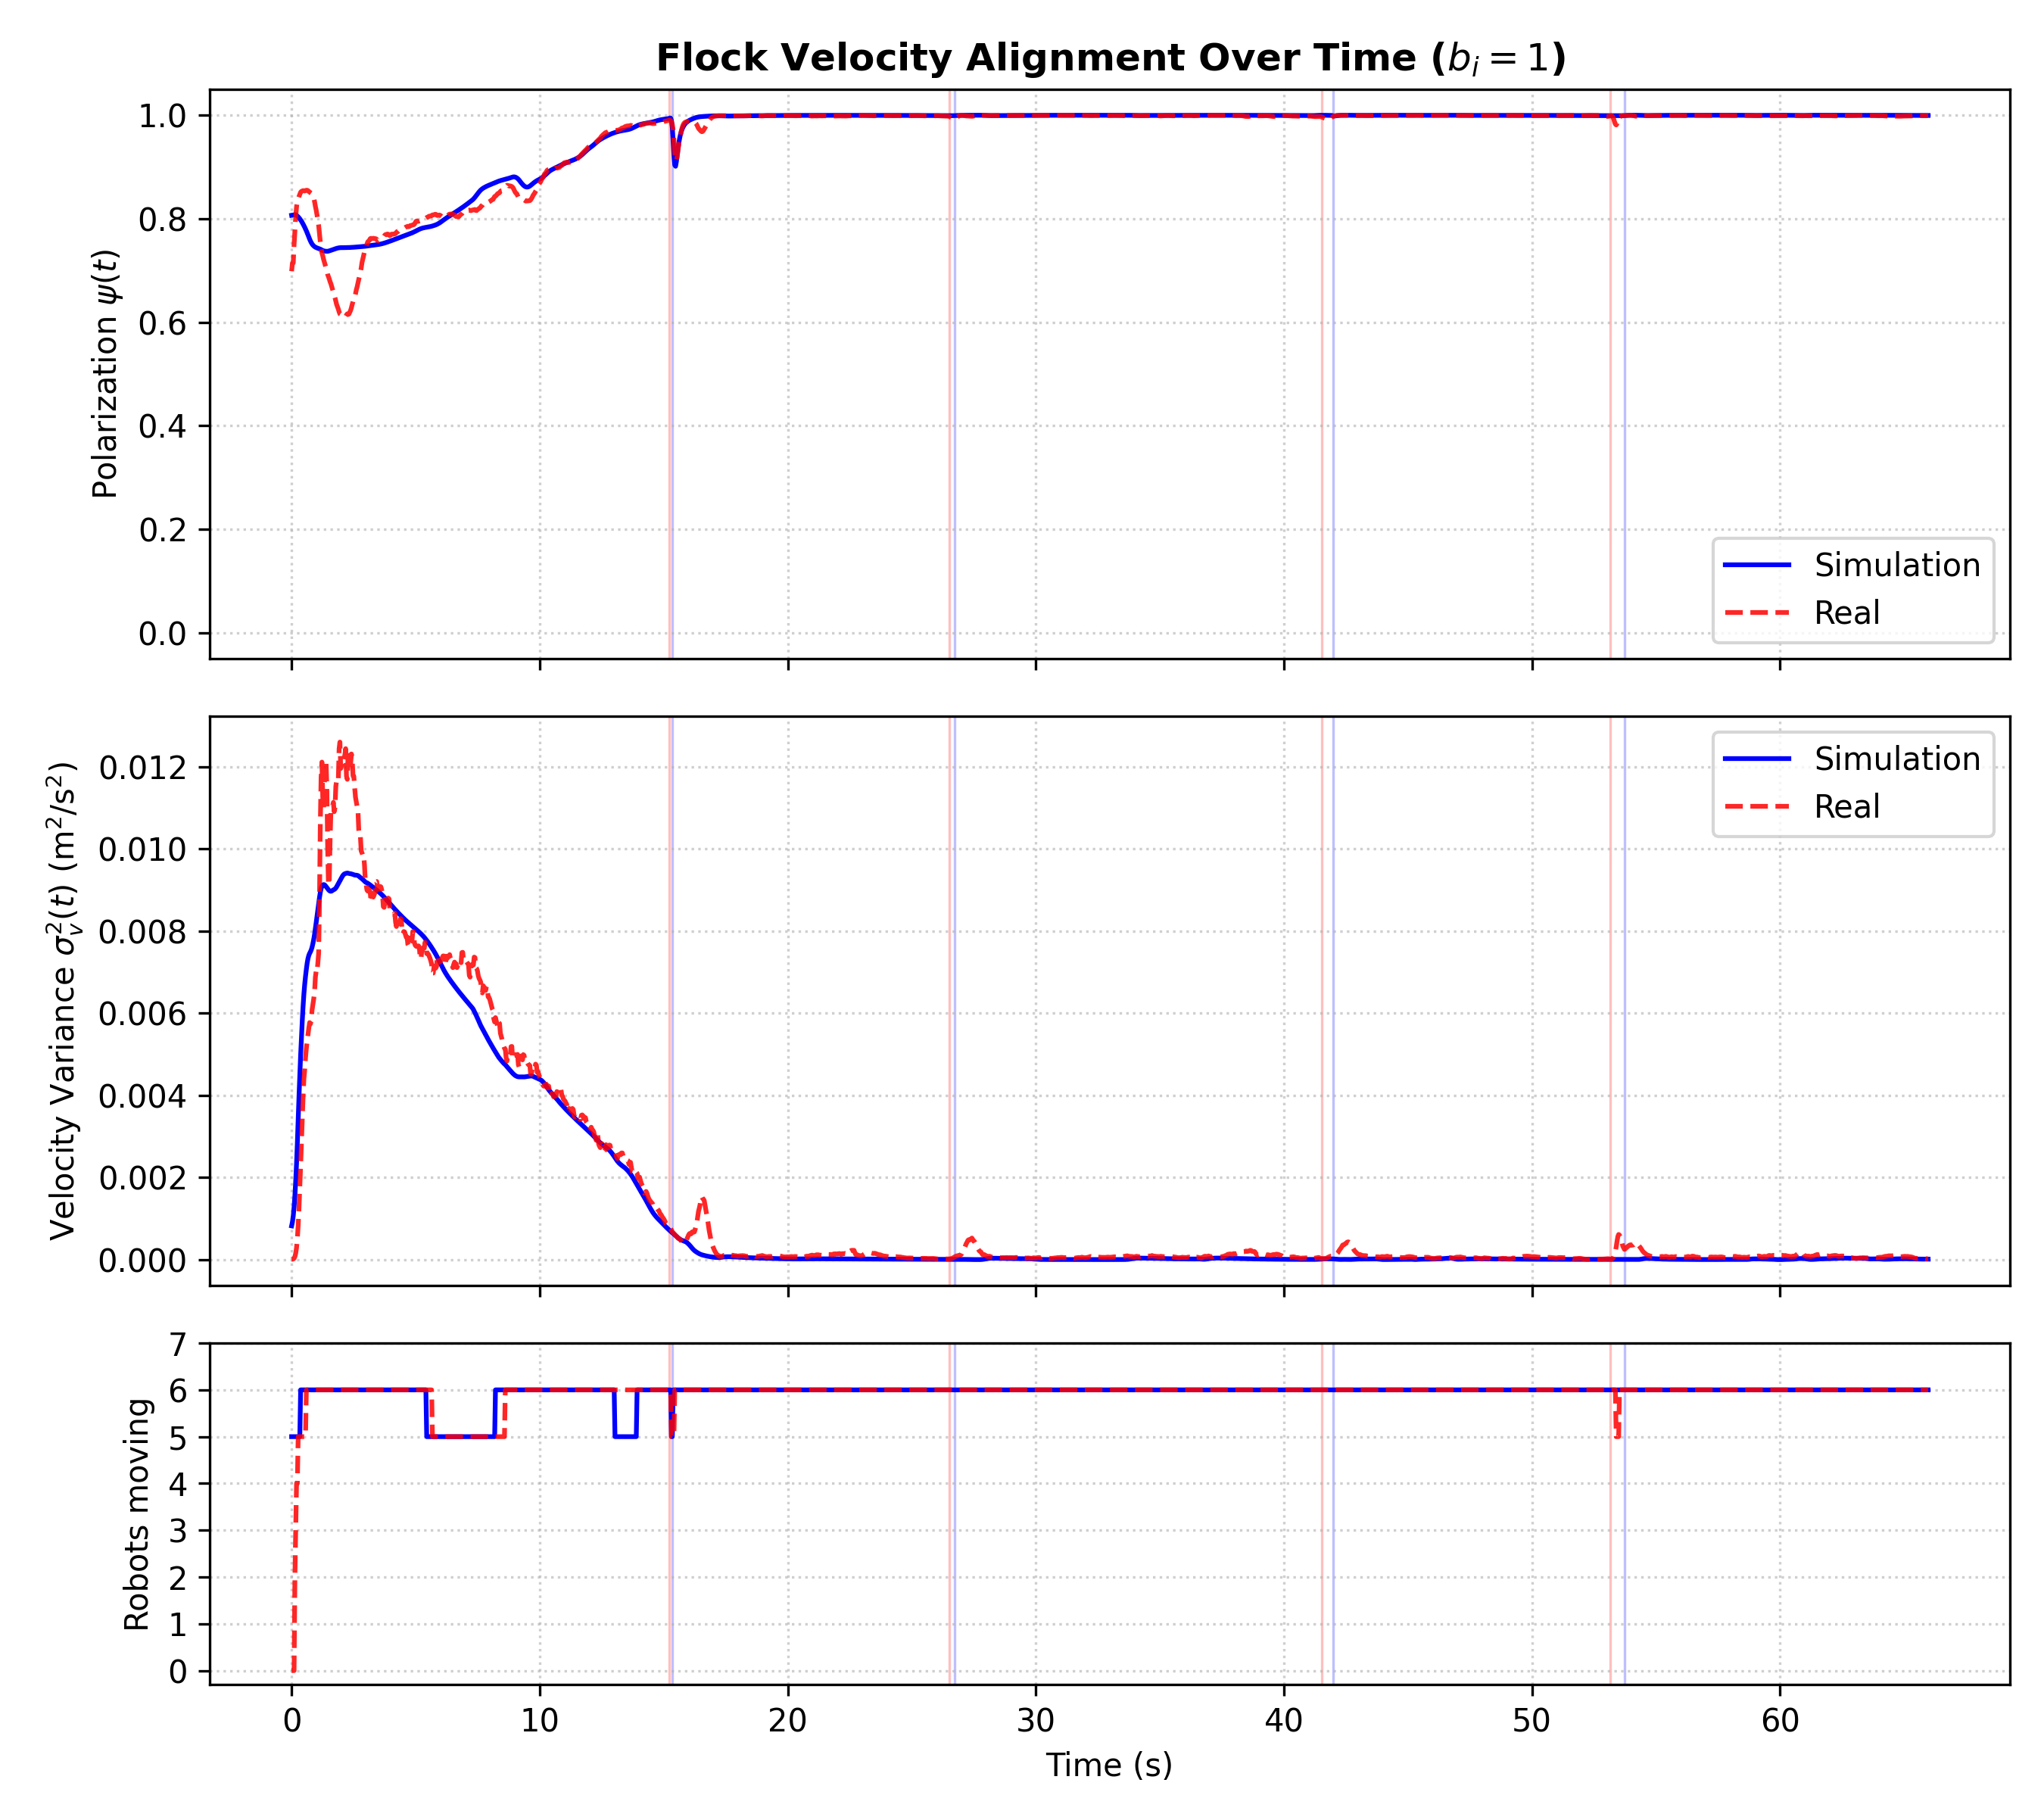
\includegraphics[width=0.8\textwidth]{Figures/part2_sec2_velocity_alignment.png}
    \captionsetup{justification=centering}
    \caption{Simulation and hardware robot velocity alignment metrics for global-knowledge flocking control.}
    \label{fig:metrics_2}
\end{figure}

Finally, the number of individual (or fragments) flock groups, maximum pairwise distance, and distance of the flock centroid from the current waypoint coordinates are provided in Figure \ref{fig:cohesion_2}. As seen, and as explored earlier, there are initially 6 flock fragments (just the robots moving independently). But, at $\sim17\ s$, when the robots enter the range of each other, the flock reduces to a single group that maintains itself throughout the experiments. The maximum pairwise distance decreases as the robots approach each other, then is steady as the balancing ``forces'' of the flock keep each robot within the same flock position relative to the other robots. Finally, the square distance between the flock centroid and the current waypoint index experiences sharp discontinuities when the waypoint shifts, exactly as was seen in formation control (Figure \ref{fig:square_way_b}). Overall, the global-knowledge flocking performs very similarly to the global-knowledge formation control, as in the robots quickly achieve their desired ``formation'' and maintain it throughout the rest of the experiment simply by all sharing the common knowledge and goal of the next waypoint. There is no true way for the formation or flock to scatter once it is formed, as they will always move in the same manner.

\begin{figure}[htb]
    \centering
    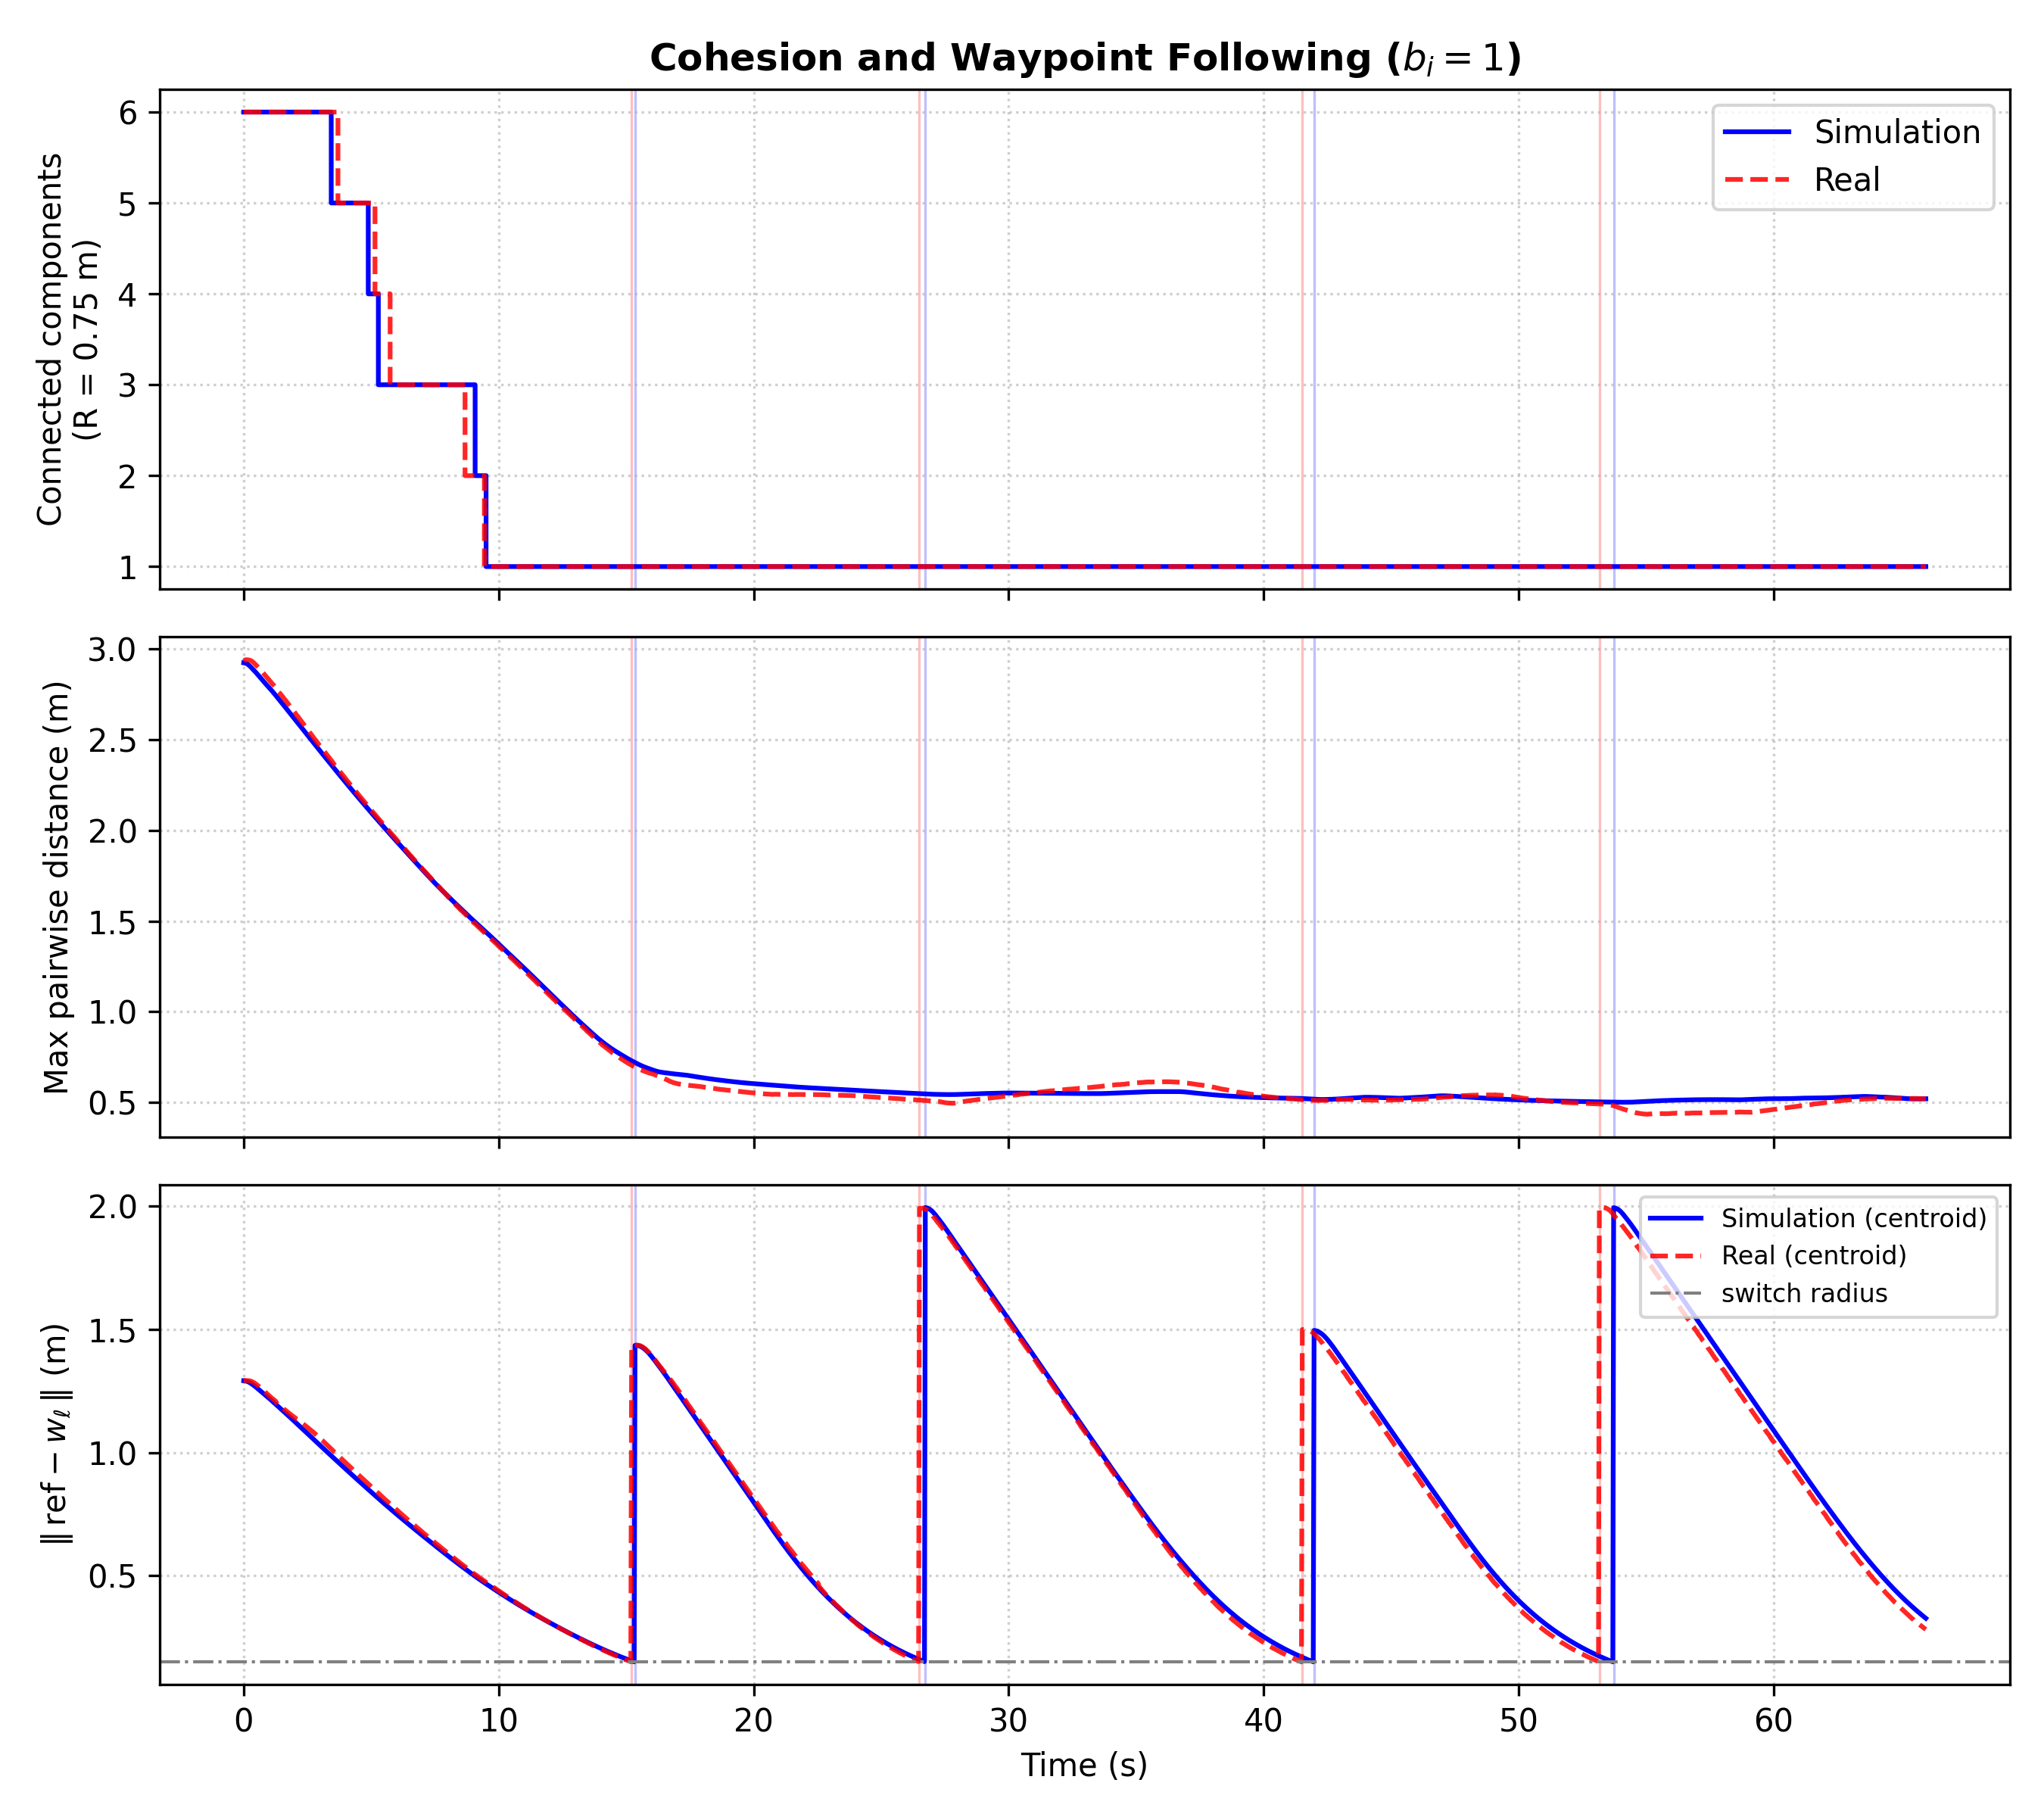
\includegraphics[width=0.8\textwidth]{Figures/part2_sec2_cohesion_waypoint.png}
    \captionsetup{justification=centering}
    \caption{Simulation and hardware robot cohesion and waypoint following metrics for global-knowledge flocking control.}
    \label{fig:cohesion_2}
\end{figure}


\clearpage
\subsection*{3.}
Select one of the existing robots as a leader: set $b_i=1$ for the leader and $b_i=0$ for all others (this means only the leader receives waypoint information). Repeat the experiments and plots, keeping the initial conditions and parameters unchanged. How does limited reference information affect waypoint following, cohesion, and velocity alignment?

\subsection*{ANSWER:}
The flocking experiment was repeated with a leader-follower paradigm, where only one of the existing robots has knowledge of the waypoints. In this case, the waypoint was switched when the \textit{leader} entered an appropriate distance of the waypoint. Figure \ref{fig:traj_3} shows the trajectories for this leader-follower flocking experiments for both the simulation and physical hardware, and as seen, they are very similar (the square error is given in Figure \ref{fig:square_3}, which, as in all the previous cases, grows with time due to the accumulation of discrepancies between the simulator and physical system). What was interesting about this experiment compared to the global-knowledge flocking was that, since all robots were initialized with $v_i[k]0$, \textit{all of the followers remained stationary until the leader ``picked them up''!} Additionally, while it may be difficult to observe when just considering the trajectories, as only the leader has incentive to move towards the next waypoint, this caused a ``lagging'' effect where the rest of the flock moved behind the leader, being pulled along only through the cohesion and velocity alignment terms of the algorithm. However, once the flock was formed, it did maintain cohesion throughout, just not as seamlessly as during the global-knowledge flocking experiments.

\begin{figure}[htb]
    \centering
    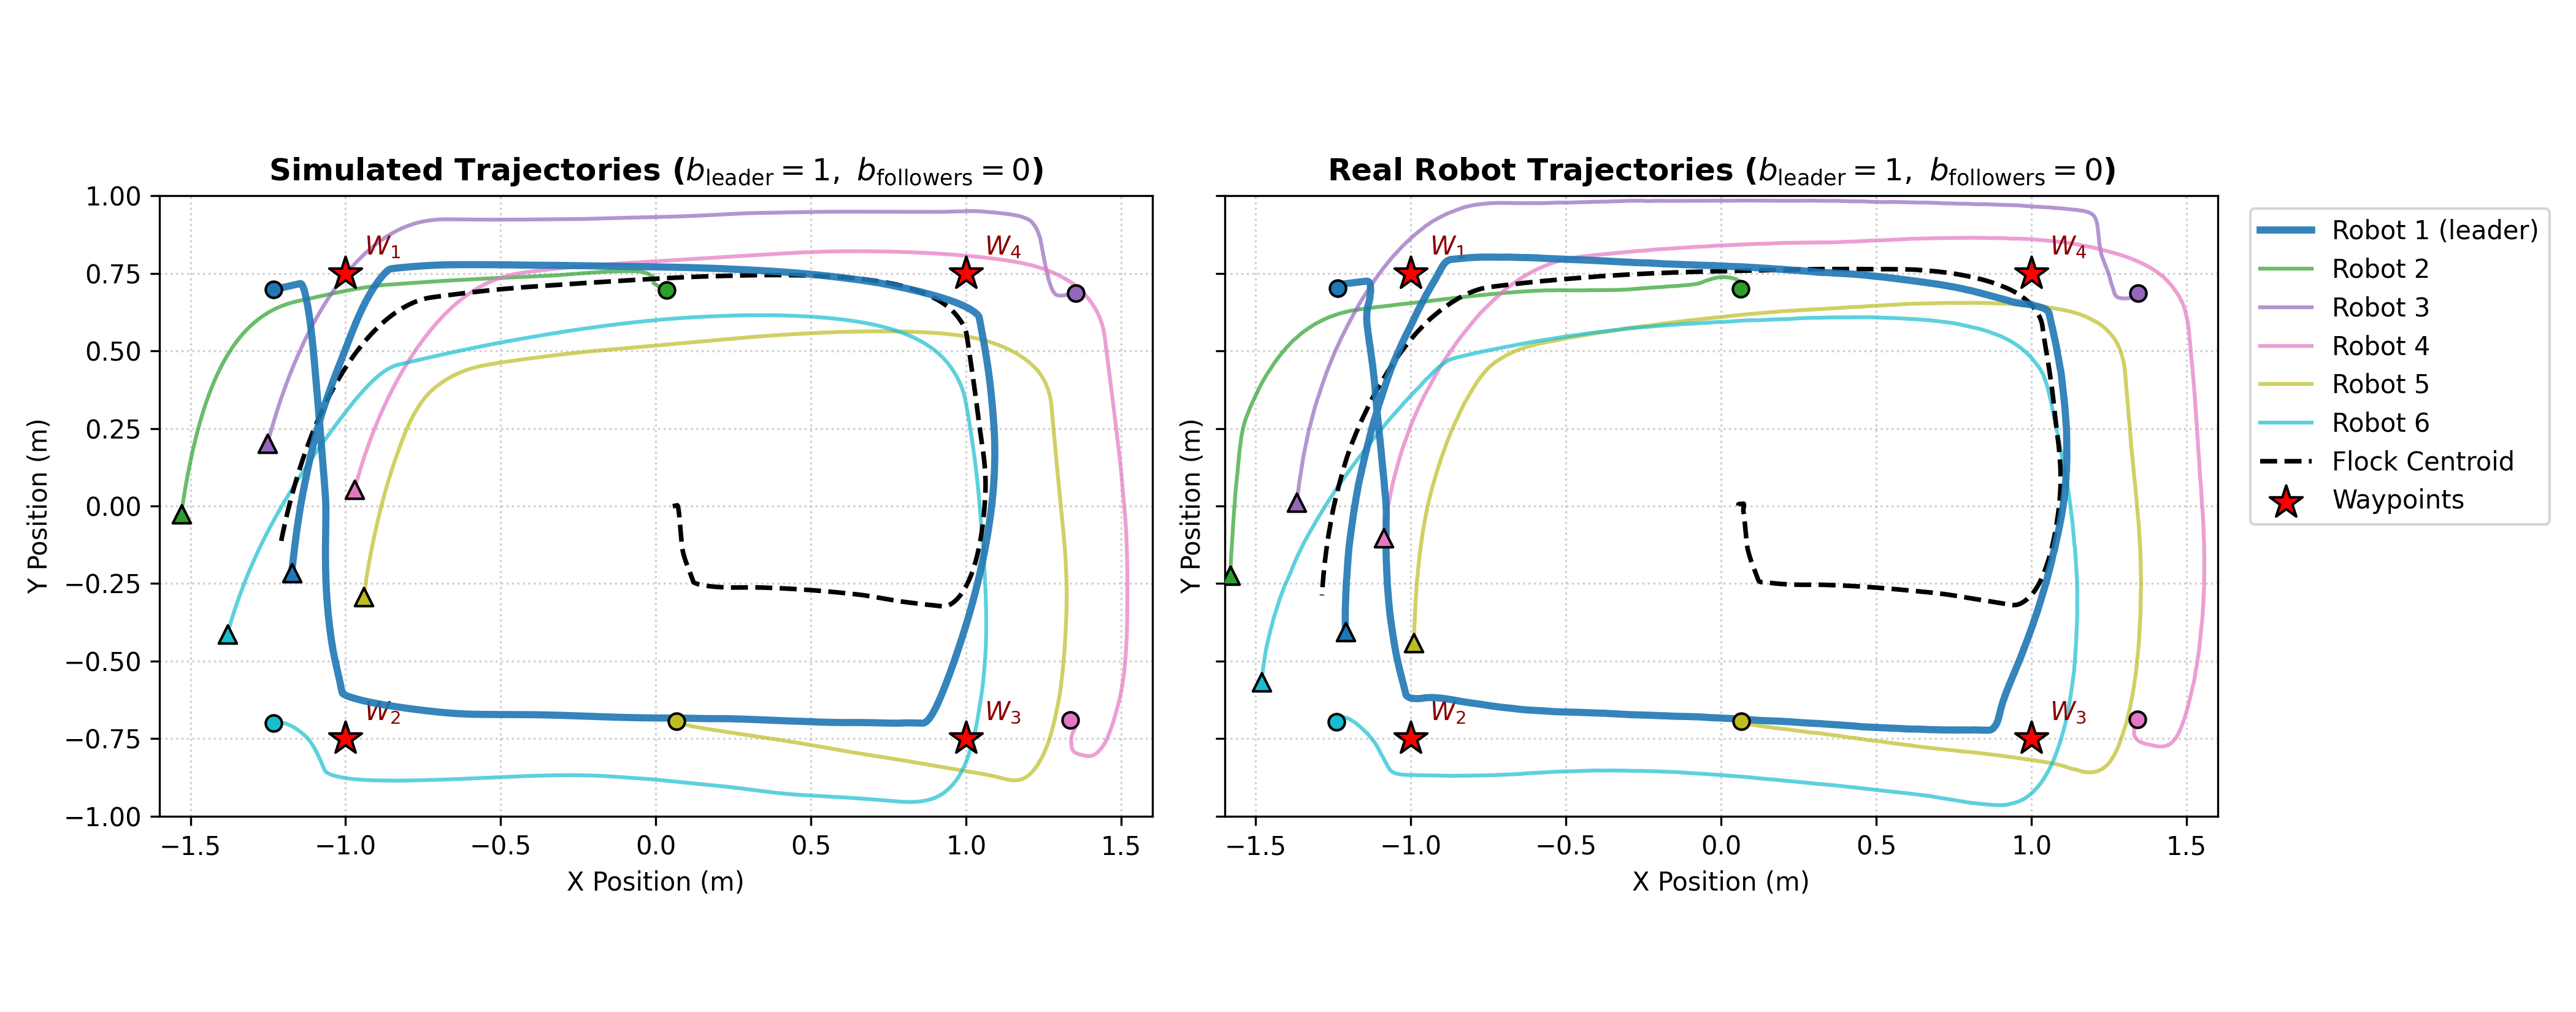
\includegraphics[width=0.9\textwidth]{Figures/part2_sec3_trajectories.png}
    \captionsetup{justification=centering}
    \caption{Simulation and hardware robot trajectories for leader-follower flocking control.}
    \label{fig:traj_3}
\end{figure}

\begin{figure}[htb]
    \centering
    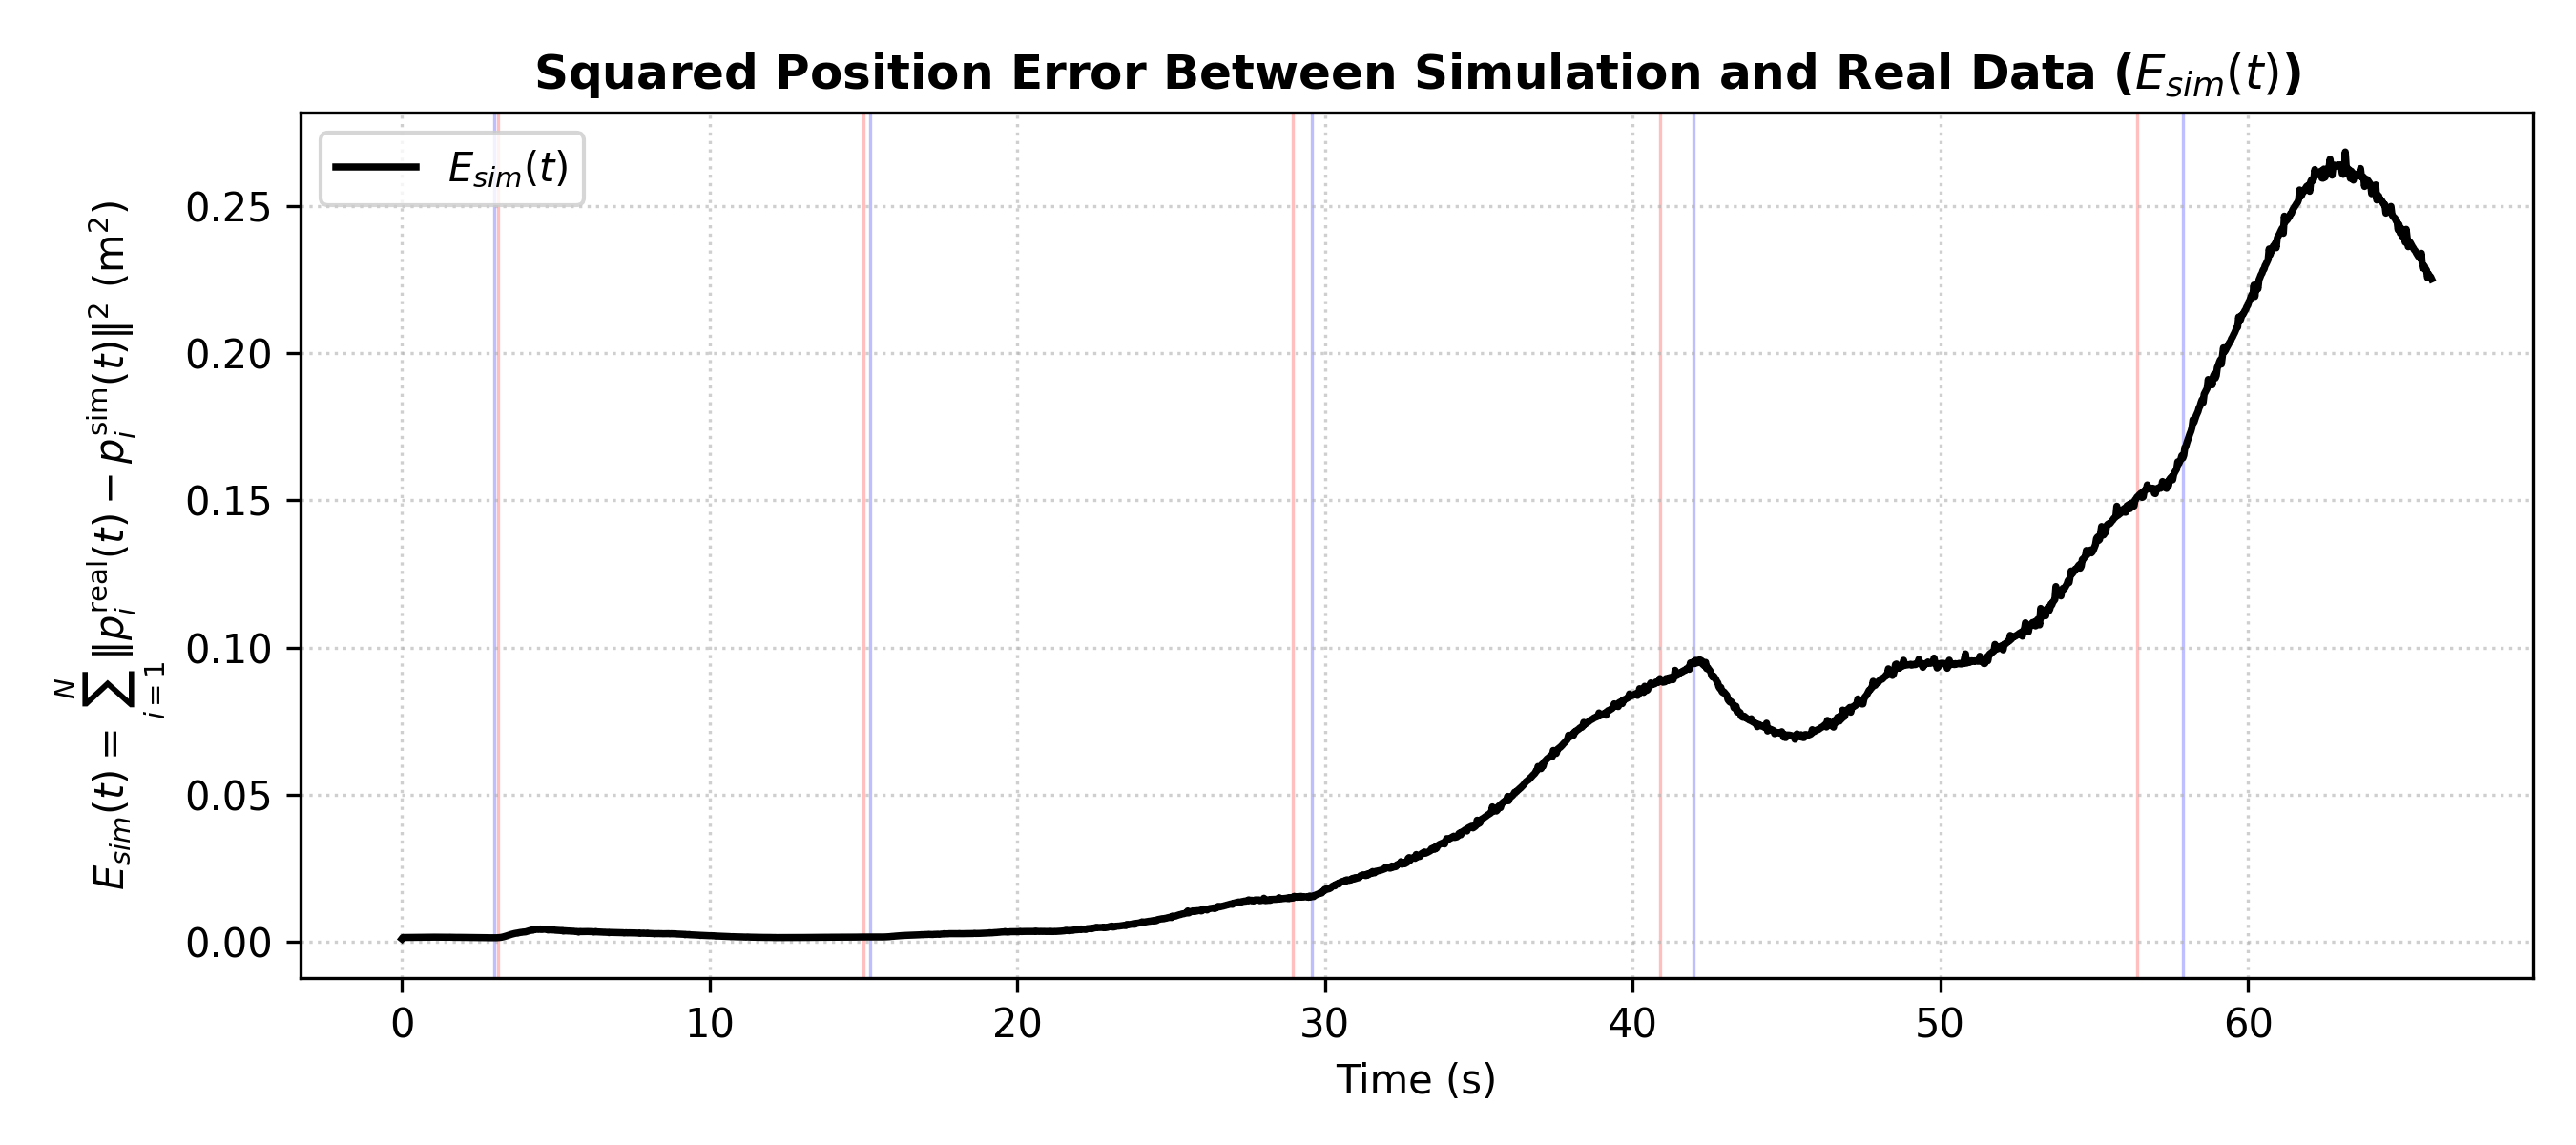
\includegraphics[width=0.8\textwidth]{Figures/part2_sec3_E_sim.png}
    \captionsetup{justification=centering}
    \caption{Square error between $p^{real}(t)$ and $p^{sim}(t)$ for leader-follower flocking control.}
    \label{fig:square_3}
\end{figure}

\FloatBarrier
Figure \ref{fig:metrics_3} displays the velocity alignment metrics for the leader-follower experiments. As seen, while the polarization $\psi(t)$ was near 1 for the entire duration of the experiment, that was because \textit{no} robots were moving until they joined the flock. At that point, upon joining the flock, there is a slight ``dip'' in the polarization as the new robot acclimates to the flocks velocity, but then harmony is restored. The velocity variance $\sigma_v^2(t)$, however, is much more sporadic than the results in Figure \ref{fig:metrics_2}, as robots that are not moving contribute to the error in this metric. It is not until $\sim 45\ s$, when the last robot is ``picked up'' (as seen by the number of robots moving) that the variance reduces near 0, with only a minor hiccup as the next waypoint is triggered at $\sim 56\ s$ and the leader changes directions, forcing the followers to adapt. In terms of metrics, this method performs worse than the global-knowledge, which should not be a surprise, as the followers only receive information from the leader, but it has the advantage of not needed a shared global plan. 

\begin{figure}[htb]
    \centering
    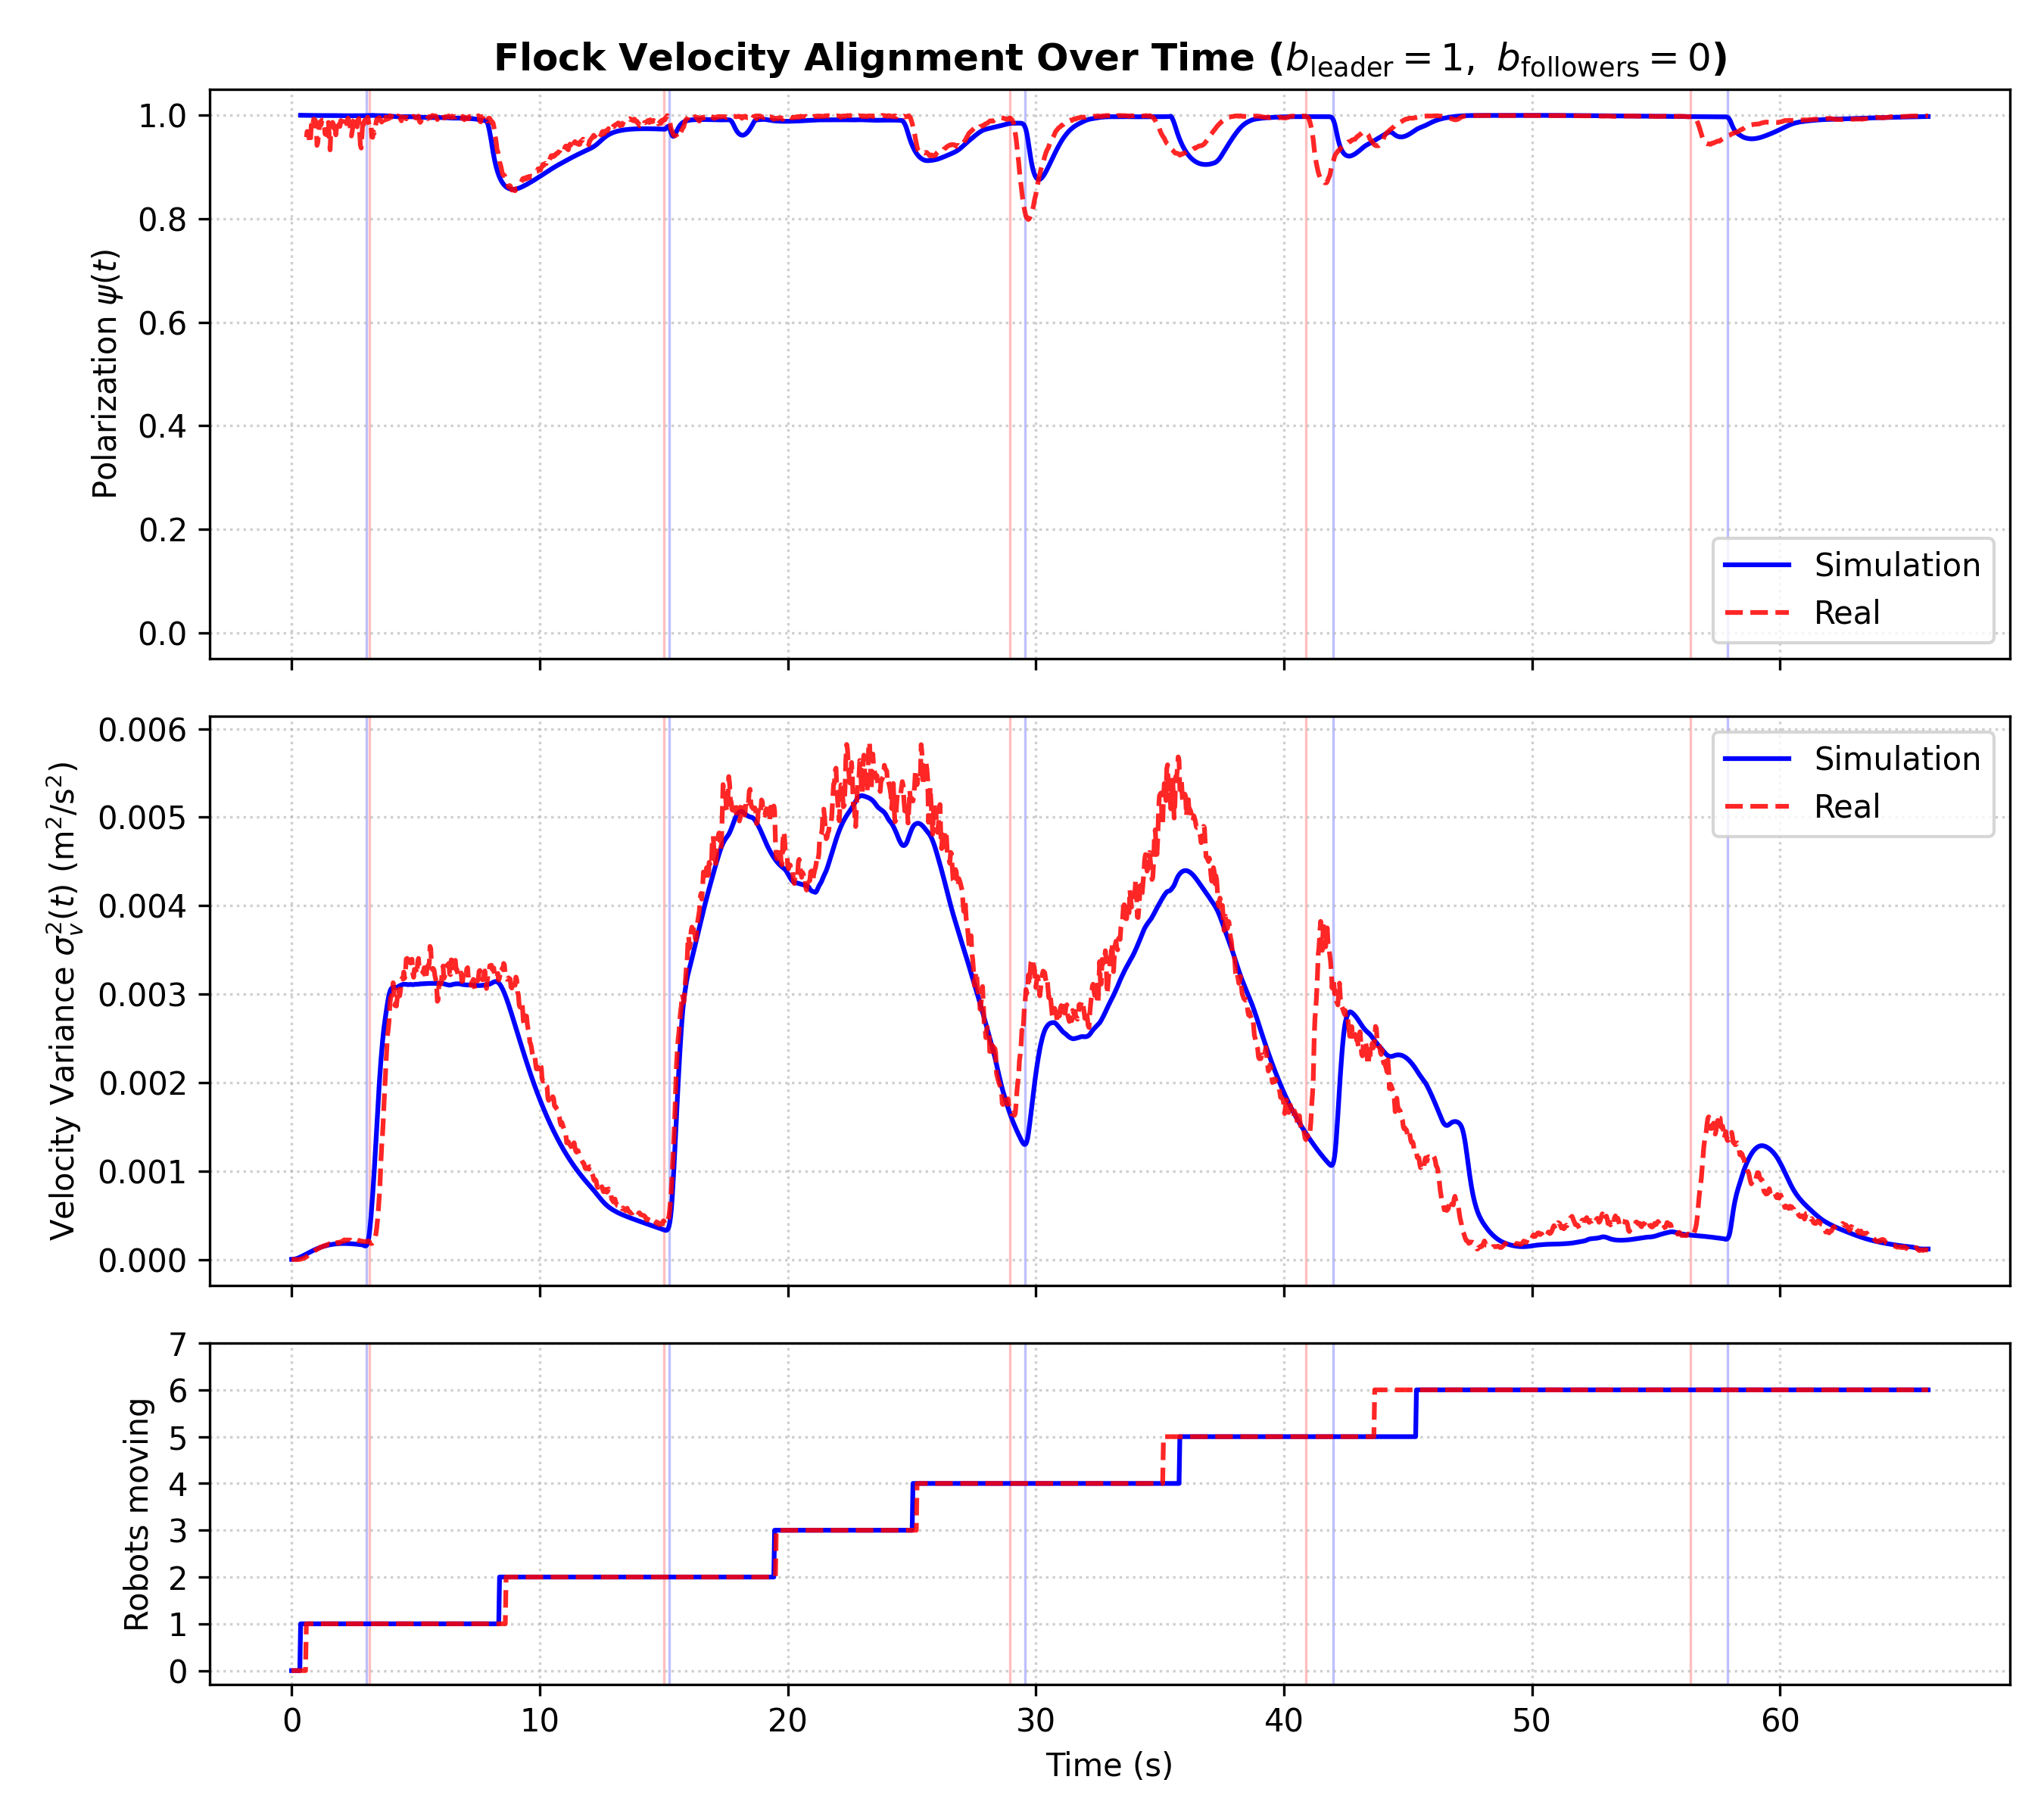
\includegraphics[width=0.8\textwidth]{Figures/part2_sec3_velocity_alignment.png}
    \captionsetup{justification=centering}
    \caption{Simulation and hardware robot velocity alignment metrics for leader-follower flocking control.}
    \label{fig:metrics_3}
\end{figure}

Figure \ref{fig:cohesion_3} provides the number of flock fragments, maximum pairwise distance, and distance of the flock centroid from the current waypoint coordinates. As seen, the number of connected components is much slower to reduce to 0 than during the global-knowledge case (Figure \ref{fig:metrics_2}). This is from the ``picking up'' behavior that the system displayed, as each robot remained stationary in its own fragment of the flock until the leader came within appropriate sensing range. Additionally, the maximum pairwise distance is much slower to reduce for the same reason, but inevitably reaching a similar value as during the global-knowledge case. While it is slower to converge than the global-knowledge (again, not surprising, especially in the case where all robots begin stationary), it does eventually reach a similar performance.

\begin{figure}[htb]
    \centering
    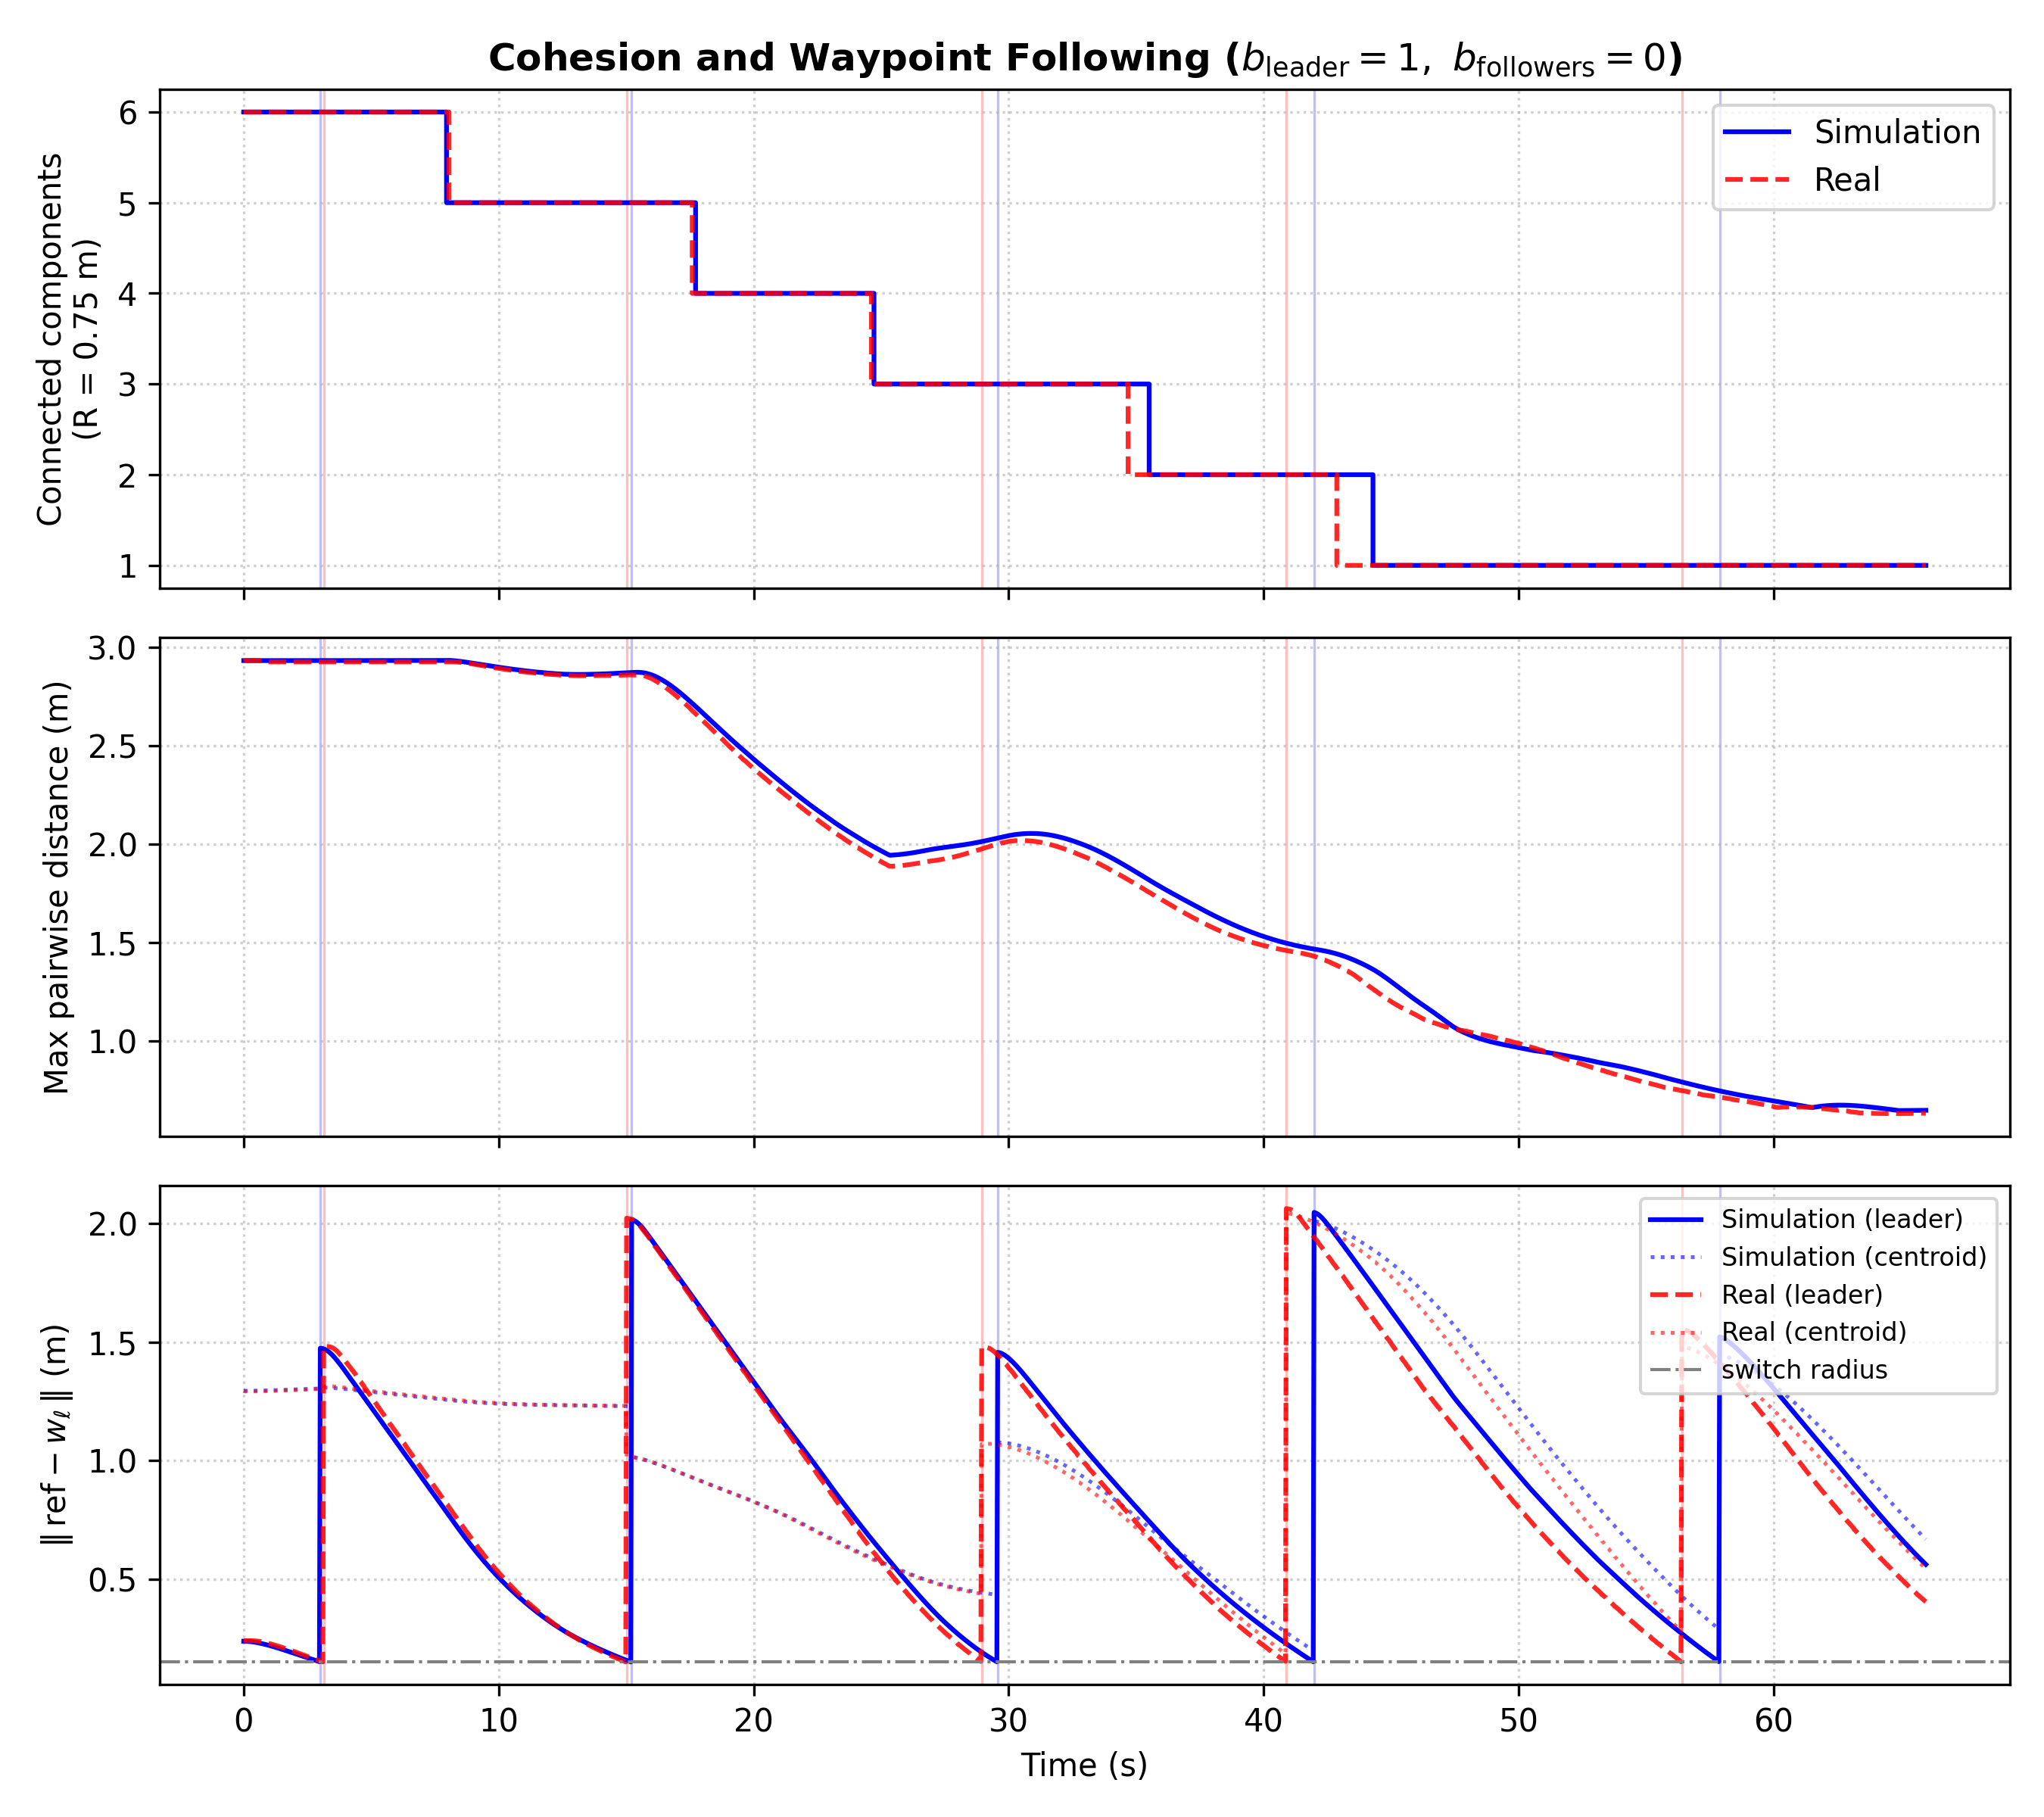
\includegraphics[width=0.8\textwidth]{Figures/part2_sec3_cohesion_waypoint.png}
    \captionsetup{justification=centering}
    \caption{Simulation and hardware robot cohesion and waypoint following metrics for leader-follower flocking control.}
    \label{fig:cohesion_3}
\end{figure}

%%%%% REFERENCES
% \clearpage
% \printbibliography[title={\textbf{REFERENCES}}]

%%%% APPENDIX
\appendix\appendixpagenumbering
\section{CODE}\label{app:code}
\subsection{Part A. and C.: simulation loop}
\begin{minted}[fontsize=\footnotesize, breaklines]{python}
for t in range(config.ac_iterations): # for each time step
    poses = r.get_poses() # get all poses of robots
    velocities = np.zeros((2, config.ac_N)) # create empty velocity array

    if config.c_proximity: Ap = GraphProximity(poses=poses, radius=config.c_radius) # if proximity-based, find new adjacency

    # updating robot commands
    for i in range(config.ac_N): # for each robot
        if config.c_proximity: neighbors = topological_neighbors(L=Ap, agent=i) # find all neighbors for proximity Laplacian
        else: neighbors = topological_neighbors(L=L, agent=i) # find all neighbors for static Laplacian

        for j in neighbors: # for each neighbor
            if config.a_distance == True: # distance formation control
                a_distance = np.linalg.norm(poses[:2,i] - poses[:2,j]) # find current distance between i and j
                d_distance = config.ac_dmatrix[i,j] # find desired distance between i and j

                velocities[:,i] += config.ac_formation_gain * (a_distance**2 - d_distance**2) * (poses[:2,j] - poses[:2,i]) # add to velocity command

            else: # displacement formation control
                velocities[:,i] += config.ac_formation_gain * ((poses[:2,j] - config.ac_disp[j,:]) - (poses[:2,i] - config.ac_disp[i,:])) # add to velocity command

    # velocity saturation
    speeds = np.linalg.norm(velocities, axis=0) # find current speed of each robot
    speed_threshold = config.linear_velocity_limit * r.MAX_LINEAR_VELOCITY # determine threshold value
    threshold_idx = speeds > speed_threshold # find speeds that surpass threshold
        
    if np.any(threshold_idx): # if there are any to saturate
        velocities[:,threshold_idx] *= speed_threshold / speeds[threshold_idx] # apply speed reduction

    # safety and dynamics application
    velocities = si_barrier_cert(dxi=velocities, x=poses[:2,:]) # ensure there are no collisions
    inputs = si_to_uni_dyn(dxi=velocities, states=poses) # convert to proper control inputs

    # step forward simulation
    r.set_velocities(ids=np.arange(config.ac_N), velocities=inputs) # set control velocities
    r.step() # step forward time

    # collect data
    data_poses.append(poses) # add poses to array
\end{minted}

\clearpage
\subsection{Part B: simulation loop}
\begin{minted}[fontsize=\footnotesize, breaklines]{python}
for t in range(config.b_iterations): # for each time step
    poses = r.get_poses() # get all poses of robots
    velocities = np.zeros((2, config.b_N)) # create empty velocity array

    # updating robot commands
    if config.b_leader: # if using a leader
        for i in range(config.b_N): # for each robot
            neighbors = topological_neighbors(L=L, agent=i) # find all neighbors
            for j in neighbors: # for each neighbor
                a_distance = np.linalg.norm(poses[:2,i] - poses[:2,j]) # find current distance between i and j
                d_distance = config.b_dmatrix[i,j] # find desired distance between i and j

                velocities[:,i] += config.b_formattion_gain * (a_distance**2 - d_distance**2) * (poses[:2,j] - poses[:2,i]) # add to velocity command
    
        # update leader pose
        velocities[:,0] = leader_controller(states=poses[:2,0].reshape(2,1), poses=np.reshape(config.b_waypoints[waypoint_idx,:],(2,1))).flatten()

        # update waypoint state
        if np.linalg.norm(poses[:2,0] - config.b_waypoints[waypoint_idx,:]) < config.b_waypoint_tol:
            waypoint_idx = (waypoint_idx + 1) % config.b_waypoints.shape[0] # wrap waypoint index
    
    else: # if all know plan
        # find average formation position
        average = PosesAverage(poses=poses)

        for i in range(config.b_N): # for each robot
            velocities[:,i] = -config.b_formattion_gain * (poses[:2,i] - (config.b_disp[i,:] + reference_pose)) # add to velocity command

        # update reference pose
        reference_pose += 0.033 * leader_controller(states=reference_pose.reshape((2,1)), poses=np.reshape(config.b_waypoints[waypoint_idx,:],(2,1))).flatten()

        # update waypoint state
        if np.linalg.norm(reference_pose - config.b_waypoints[waypoint_idx,:]) < config.b_waypoint_tol:
            waypoint_idx = (waypoint_idx + 1) % config.b_waypoints.shape[0] # wrap waypoint index

    # velocity saturation
    speeds = np.linalg.norm(velocities, axis=0) # find current speed of each robot
    speed_threshold = config.linear_velocity_limit * r.MAX_LINEAR_VELOCITY # determine threshold value
    threshold_idx = speeds > speed_threshold # find speeds that surpass threshold
        
    if np.any(threshold_idx): # if there are any to saturate
        velocities[:,threshold_idx] *= speed_threshold / speeds[threshold_idx] # apply speed reduction

    # safety and dynamics application
    velocities = si_barrier_cert(dxi=velocities, x=poses[:2,:]) # ensure there are no collisions
    inputs = si_to_uni_dyn(dxi=velocities, states=poses) # convert to proper control inputs

    # step forward simulation
    r.set_velocities(ids=np.arange(config.b_N), velocities=inputs) # set control velocities
    r.step() # step forward time

    # collect data
    data_poses.append(poses) # add poses to array
    data_waypoint_pose.append(np.append(waypoint_idx, config.b_waypoints[waypoint_idx,:])) # add waypoint idx to array
    if not config.b_leader: # if not using leader
        data_average_pose.append(average) # add average to array
        data_reference_pose.append(np.copy(reference_pose)) # add reference pose to array
\end{minted}

\clearpage
\subsection{Helper functions}
\begin{minted}[fontsize=\footnotesize, breaklines]{python}
##### GRAPH ADJACENCY FUNCTION (generates graph adjacency matrix for given weight matrix)
def GraphAdjacency(W: np.ndarray) -> np.ndarray:
    # creating empty array
    A = np.zeros(np.shape(W))

    # construc adjacency
    for row_idx, row in enumerate(W): # for every row
        for col_idx, ele in enumerate(row): # for every column
            if ele != 0: A[row_idx,col_idx] = 1 # set adjacency weight

    # return A
    return A

##### GRAPH IN-DEGREE FUNCTION (inputs graph adjacency and returns in degree matrix)
def GraphInDegree(A: np.ndarray) -> np.ndarray:
    # sum over all rows and return diagonal matrix
    return np.diag(np.sum(A, axis=1))

##### GRAPH LAPLACIAN FUNCTION (inputs distance weight matrix and generates proper graph Laplacian)
def GraphLaplacian(W: np.ndarray) -> np.ndarray:
    # creating adjacency matrix
    A = GraphAdjacency(W=W)

    # finding indegree matrix
    D = GraphInDegree(A=A)

    # return L
    return D - A

##### GRAPH-PROXIMITY FUNCTION (inputs robot current positions and communication radius and generates proximity-based Laplacian matrix)
def GraphProximity(poses: np.ndarray, radius: float) -> np.ndarray:
    # create empty adjacency matrix
    _, N = np.shape(poses) # find number of robots
    Ap = np.zeros((N, N)) # empty matrix

    # constructing proximity adjacency
    for i in range(N): # for each robot
        for j in range(i+1, N): # for each other robot
            a_distance = np.linalg.norm(poses[:2,i] - poses[:2,j]) # find current distance between i and j
            if a_distance < radius: # if robots are within proximity of each other
                Ap[i,j] = 1 # update element
                Ap[j,i] = 1 # update symmetric element

    # return adjacency
    return Ap

##### GRAPH RIGIDITY FUNCTION (inputs weight matrix and desired positions and returns rigidity matrix and rank)
def GraphRigidity(W: np.ndarray, positions: np.ndarray) -> tuple[np.ndarray, float]:
    # finding number graph nodes
    N, _ = np.shape(W)

    # finding number of graph edges
    A = GraphAdjacency(W=W) # gives 1 where there is an edge between nodes
    E = int(np.sum(A) / 2) # sum all 1s and divide by 2 for double counting

    # create rigidity matrix
    R = [] # empty array
    for i in range(N): # for each robot
        for j in range(i + 1, N): # for each other robot beyond i
            if A[i,j] != 0: # if there is an edge
                R_row = np.zeros(2 * N) # create row of all 0s

                diff = positions[i,:] - positions[j,:] # find distance between positions

                # update row elements
                R_row[2*i] = diff[0]
                R_row[2*i + 1] = diff[1]
                R_row[2*j] = -diff[0]
                R_row[2*j + 1] = -diff[1]

                R.append(R_row) # append to final rigidity matrix

    R = np.array(R) # transform into an array
    rank = np.linalg.matrix_rank(R) # find rank

    # return results
    return R, rank

##### AVERAGE POSITION FUNCTION
def PosesAverage(poses: np.ndarray) -> np.ndarray:
    # find number of robots
    _, N = np.shape(poses)

    # find average x and y positions
    x = np.sum(poses[0,:]) / N
    y = np.sum(poses[1,:]) / N

    # return value
    return np.array([x, y])
\end{minted}

\clearpage
\subsection{Error calculation functions}
\begin{minted}[fontsize=\footnotesize, breaklines]{python}
##### ERROR DISTANCE CONSTRAINT FUNCTION (inputs distance matrix and agent positions and returns error)
def ErrorDistanceConstraint(W: np.ndarray, poses: np.ndarray) -> float:
    # finding number of graph edges and nodes
    # finding number graph nodes
    N, _ = np.shape(W)
    A = GraphAdjacency(W=W) # gives 1 where there is an edge between nodes
    E = int(np.sum(A) / 2) # sum all 1s and divide by 2 for double counting

    # calculating the error
    error = 0 # initially 0 error
    for i in range(N): # for each robot 
        for j in range(i + 1, N): # for each other robot
            if A[i,j] != 0: # if there is an edge
                a_distance = np.linalg.norm(poses[:2,i] - poses[:2,j]) # find current distance between i and j
                d_distance = W[i,j] # find desired distance between i and j

                error += (a_distance - d_distance) ** 2 # add to error sum

    return np.sqrt(error / E) # return final error

##### SQUARE ERROR FUNCTION (returns square error between sim and real data)
def ErrorSquare(sim_poses: np.ndarray, real_poses: np.ndarray) -> float:
    sim_poses = sim_poses.T # transpose data for easier parsing
    real_poses = real_poses.T # transpose data for easier parsing

    # calculating the error
    error = 0 # initially 0 error
    for sim_pose, real_pose in zip(sim_poses, real_poses): # for each agent's position
        error = error + np.linalg.norm(sim_pose[:2] - real_pose[:2]) ** 2

    return error # return final square error

##### REFERENCE ERROR FUNCTION (returns square error between reference pose and waypoint pose)
def ErrorReference(average_pose: np.ndarray, waypoint_pose: np.ndarray) -> float:
    # return error
    return ErrorSquare(sim_poses=np.array([average_pose]), real_poses=np.array([waypoint_pose[1:]]))
\end{minted}

\clearpage
\subsection{Visualization functions}
\begin{minted}[fontsize=\footnotesize, breaklines]{python}
##### FORMATION VISUALIZER FUNCTION (inputs desired robot positions and plots/saves formation)
def VisualFormation(positions: np.ndarray) -> plt.Figure:
    # defining constants
    workspace_width = 3.2 # (m)
    workspace_height = 2.0 # (m)

    # creating figure
    fig_form = plt.figure('Formation plot', figsize=(7,5))
    fig_form.suptitle(f'Desired agent formation\nPart A. Static-formation control')
    ax = fig_form.add_subplot(1, 1, 1)

    # adding the workspace to the plot
    workspace = patches.Rectangle((-workspace_width/2, -workspace_height/2), width=workspace_width, height=workspace_height, linewidth=2.0, edgecolor='#000000', facecolor='#999999')
    ax.add_patch(workspace)

    # adding the robots to the plot
    for robot_idx, [x, y] in enumerate(positions): # for each robot
        robot = plt.Circle((x, y), radius=0.06, facecolor='#ffffff', edgecolor='#0000ff', linewidth=1) # add position marker
        ax.add_patch(robot)
        ax.text(x, y-0.01, robot_idx, color='#000000', weight='bold', fontsize=10, ha='center', va='center') # add index

    ax.set_xlim((-workspace_width/2-0.1, workspace_width/2+0.1))
    ax.set_ylim((-workspace_height/2-0.1, workspace_height/2+0.1))
    ax.set_xlabel(r'$x$ $(m)$')
    ax.set_ylabel(r'$y$ $(m)$')
    ax.set_aspect('equal')

    # return plot
    return fig_form

##### SQUARE ERROR PLOT FUNCTION (inputs error and returns error plot)
def VisualSquareError(errors: list, legend: list, idx: int, tag: str) -> plt.Figure:
    # defining constants
    t_step = 0.033 # (s)

    # extracting errors
    if len(errors) > 1: # if plotting multiple errors
        dist_error = errors[0]
        disp_error = errors[1]
    else: error = errors[0]

    # creating figure
    fig_error = plt.figure(f'Square Error Plot {idx}', figsize=(7,5))
    fig_error.suptitle(f'Square Error versus time\n' + tag)
    ax = fig_error.add_subplot(1, 1, 1)

    # plotting data
    t = t_step * np.arange(0, len(errors[0])) # time data
    if len(errors) > 1:
        ax.plot(t, dist_error, linestyle='-', label=legend[0])
        ax.plot(t, disp_error, linestyle='--', label=legend[1])
        ax.legend(loc='best')
    else: ax.plot(t, error, linestyle='-')
    ax.set_xlabel(r'Experiment time $t$ $(s)$')
    ax.set_ylabel(r'Square Error $(m^2)$')

    # return figure
    return fig_error

##### CONSTRAINT ERROR PLOT FUNCTION (inputs error and returns plot)
def VisualConstraintError(errors: list, idx: int, tag: str) -> plt.Figure:
    # defining constants
    t_step = 0.033 # (s)

    # extracting errors
    sim_error = errors[0]
    real_error = errors[1]

    # creating figure
    fig_error = plt.figure(f'Constraint Error Plot {idx}', figsize=(7,5))
    fig_error.suptitle(f'Constraint Error versus Desired\n' + tag)
    ax = fig_error.add_subplot(1, 1, 1)

    # plotting data
    t = t_step * np.arange(0, len(errors[0])) # time data
    ax.plot(t, sim_error, linestyle='-', label=fr'Simulated')
    ax.plot(t, real_error, linestyle='--', label=fr'Real')
    ax.legend(loc='best')
    ax.set_xlabel(r'Experiment time $t$ $(s)$')
    ax.set_ylabel(r'Square Error $(m)$')

    # return figure
    return fig_error

##### TRAJECTORY PLOT FUNCTION (inputs pose data and plots trajectories)
def VisualTrajectory(poses: list, waypoints: np.ndarray, idx: int, tag: str) -> plt.Figure:
    # defining constants
    workspace_width = 3.2 # (m)
    workspace_height = 2.0 # (m)

    _, N, _ = np.shape(poses[0]) # find number of robots

    # extracting poses
    sim_poses = poses[0]
    real_poses = poses[1]
    if len(poses) > 2: # if adding reference and average
        sim_avg_poses = poses[2]
        real_avg_poses = poses[3]
        sim_ref_poses = poses[4]
        real_ref_poses = poses[5]

    # creating figure
    fig_traj = plt.figure(f'Trajectory Plot {idx}', figsize=(7,5))
    fig_traj.suptitle(f'Robot Trajectories\n' + tag)
    ax = fig_traj.add_subplot(1, 1, 1)

    # adding the workspace to the plot
    workspace = patches.Rectangle((-workspace_width/2, -workspace_height/2), width=workspace_width, height=workspace_height, linewidth=2.0, edgecolor='#000000', facecolor='#999999')
    ax.add_patch(workspace)

    # plotting waypoints
    if waypoints is not None:
        for waypoint_idx, [x, y] in enumerate(waypoints):
            waypoint = plt.Circle((x, y), radius=0.06, facecolor='#ffffff', edgecolor='#0000ff', linewidth=1) # add position marker
            ax.add_patch(waypoint)
            ax.text(x, y-0.01, waypoint_idx, color='#000000', weight='bold', fontsize=10, ha='center', va='center') # add index

    # plotting trajectories
    for i in range(N):
        if i == 0: ax.plot(sim_poses[0,i,:], sim_poses[1,i,:], linestyle='-', label=fr'Simulated')
        else: ax.plot(sim_poses[0,i,:], sim_poses[1,i,:], linestyle='-')
    ax.set_prop_cycle(None)
    for i in range(N):
        if i == 0: ax.plot(real_poses[0,i,:], real_poses[1,i,:], linestyle='--', label=fr'Real')
        else: ax.plot(real_poses[0,i,:], real_poses[1,i,:], linestyle='--')
    if len(poses) > 2: # if plotting reference and average
        ax.plot(sim_avg_poses[:,0], sim_avg_poses[:,1], linestyle='-', color='#000000', label=fr'Simulated $\bar{{p}}$')
        ax.plot(real_avg_poses[:,0], real_avg_poses[:,1], linestyle='--', color='#000000', label=fr'Real $\bar{{p}}$')
        ax.plot(sim_ref_poses[:,0], sim_ref_poses[:,1], linestyle='-', color='#00ff00', label=fr'Reference path')
        # ax.plot(real_ref_poses[:,0], real_ref_poses[:,1], linestyle='--', color='#00ff00', label=fr'Reference')
    ax.legend(loc='best')
    ax.set_xlim((-workspace_width/2-0.1, workspace_width/2+0.1))
    ax.set_ylim((-workspace_height/2-0.1, workspace_height/2+0.1))
    ax.set_xlabel(r'$x$ $(m)$')
    ax.set_ylabel(r'$y$ $(m)$')
    ax.set_aspect('equal')

    # return figure
    return fig_traj
\end{minted}

\end{document}
